\documentclass[11pt]{article}
\usepackage{debulletin,times,graphicx,url}

% this is the template for an issue of the Data Engineering Bulletin

% all packages used by any paper must be listed here
\usepackage{subfig}
\usepackage{listings}
\usepackage{caption}
\usepackage{microtype}
\usepackage{listings}
\usepackage{booktabs}
\usepackage{listings}
\usepackage{xargs}
%\PassOptionsToPackage{hyphens}{url}
%\usepackage{hyperref}
\usepackage{multirow}
\usepackage{tabularx}
\usepackage{makecell}
\usepackage{arydshln}
\usepackage{xspace}
\usepackage{tcolorbox}
\usepackage{xpatch}

\newcommand{\Hypercallback}{Hyperupcall\xspace{}}
\newcommand{\hypercallback}{hyperupcall\xspace{}}
\newcommand{\hide}[1]{}

\begin{document}


% please enter real date, vol no, issue no
\bulletindate{March 2019}
\bulletinvolume{42}
\bulletinnumber{1}
\bulletinyear{2019}

% these are files that I have- but your part of the issue can be done without
% them
\IEEElogo{cs.pdf}
\insidefrontcover{incvA19.pdf}
%\insidebackcover[ICDE Conference]{./calls/icde-new-a.ps}

\begin{bulletin}

% the above samples assume the issue is generated from a directory structure of the following sort
% major directory name is month and year of issue
% there are sub-directorys for
% letters: directory name is "letters"
% technical articles: a directory per paper, named for an "author"
% news articles: directory name is "news"
% calls: directory name is "calls

%
%  Editor letters section.  Use the lettersection environment.
%  Each letter is contained in a letter environment, where the two required
%  options to \begin{letter} are the author and the address of the author.
%

\begin{lettersection}

% there will be other letters- and a blank page will appear in your document
% but the special issue part will be fine

\begin{letter}{Letter from the Editor-in-Chief}
{Haixun Wang}{WeWork Corporation}
\documentclass[11pt]{article} 

\usepackage{deauthor,times,graphicx}
%\usepackage{url}
\usepackage{hyperref}

\begin{document}
Around the time we published our last issue in March, the nation went
into a lockdown. Life in the last 3 months has been unprecedented in
many ways. As governments around the world scrambled to fight
coronavirus, people in the scientific community, especially those on
the frontline -- doctors, healthcare professionals, medical staff and
researchers -- made heroic efforts and sacrifices to curb the pandemic
and save lives. The data management and data science communities also
sprang to action immediately. Globally, it is the first time that data
driven approaches are being used at such a large scale toward solving
a common problem. Under this backdrop, in this special issue of the
Data Engineering Bulletin edited by Joseph Gonzalez, we feature 8
papers on the topic of {\it digital contact tracing}, a technique that
may prove crucial in the fight against Covid-19.

This issue also features two opinion pieces. Divyakant Agrawal and Amr
El Abbadi's wake-up call on managing data in an untrusted environment
takes us to the fascinating world of cryptocurrencies and
blockchains. It shows what the database community, which was
responsible for creating and perfecting transaction management and
distributed systems, can learn from the blockchain approach when it
comes to handling untrusted behaviours from the underlying
infrastructure. The second opinion piece, written by Jeffrey
D. Ullman, addresses a question on the mind of every data management
person: What is our role in the machine learning and AI revolution?
Have we missed the boat again and become irrelevant? Ullman's
perspective, illustrated by his remake of the well known Conway Venn
Diagram that illustrates the relationship between computer science,
mathematics \& statistics, and domain knowledge is incisive,
thought-provoking, and entertaining at the same time.
\end{document}


\end{letter}
%
\newpage
%
%% your introductory letter goes here
%
\begin{letter}{Letter from the Special Issue Editor}
{Philippe Bonnet}{IT University of Copenhagen}
\documentclass[11pt]{article} 

\usepackage{deauthor,times,graphicx}
%\usepackage{url}



\begin{document}

The layering of applications, database systems, operating system, and hardware,
has never been an ideal separation. For decades, database systems have overriden 
operating system services in order to efficiently support transactional properties.
However, this layering has enabled the independent evolution of database systems based on 
well-defined abstractions, at a performance cost that has remained negligible for decades.

Today, this layering is
challenged. First, applications that require low latency in addition to high throughput
cannot tolerate inefficiencies due to layer independance. When every micro-second counts,
it makes sense to streamline the data path across layers.
Second, techniques and policies devised for multicore CPUs, might have to be revised for large number
of possibly diverse cores. Third, the dominance of virtualized environments and the emergence of 
programmable hardware requires novel abstractions.

There is a need to rethink the boundaries of applications, database systems, operating system,
and hardware and revisit the nature of the interactions across these layers. In this issue, we have collected 
six articles that illustrate various forms of cross-layer support. 

The first article proposes to share information across layers to optimize resource utilization. It is
based on experimental results with SAP HANA and proposes a concrete instance of co-design between Database 
and Operating System. It identifies the need to bridge the semantic gap between application and database system.

The second article illustrates a mechanism, hyperupcalls, specifically designed to bridge such a semantic gap.
Hyperupcalls have been designed to bridge the semantic gap between a hypervisor and a guest virtual machine 
(this work got the best paper award at Usenix ATC 2018). In this paper, the authors explore how hyperupcalls
could be used from the perspective of applications and database systems.

Following these two articles from industrial research, the following three articles are authored by young
faculty members. Each outlines an ambitious research agenda that 
revisits the role of database systems on the data, control, and compute planes of modern computers.

The third article revisits operating system support for data management on modern hardware. It argues for
new forms of interface between database system and operating system.
The fourth article focuses on specialized hardware and the opportunities this creates for database system design.
The fifth article details the challenge of utilizing server cores efficiently for data intensive tasks, especially
on servers equipped with many/diverse cores, and makes the case for cross-layer support for data-intensive
task scheduling.

The sixth article focuses on a general purpose synchronization method, optimistic lock coupling, that is both
simple and scales to a large number of cores. This method is applicable to most tree-like data structures and
should be considered as an operating system-level facility on multi-core CPUs.

The traditional layering has favoured contributions from independent communities. The cross-layer approaches
outlined in this issue, favour collaborations between database experts and experts on
hardware, operating systems, compilers, and programming languages. 
We anticipate that the data engineering community will increasingly engage with these communities in the near
future.

\end{document}




\end{letter}

\end{lettersection}

% put the name of your special issue below

\begin{opinionsection}
\begin{opinion}{Data Caching Systems Win the Cost/Performance Game}
{David Lomet}{Microsoft Research, Redmond, WA 98052}
\documentclass[11pt]{article} 

\usepackage{deauthor,times,graphicx}
%\usepackage{url}
\usepackage{hyperref}


\begin{document}
%\title{Data Caching Systems Win the Cost/Performance Game}

%\author{David Lomet\\Microsoft Research\\Redmond, WA 98052\\lomet@microsoft.com}
 

%\maketitle

\section{Introduction}

\subsection{Cost/Performance}

Data in traditional data caching record management systems resides on secondary storage, and is read into main memory only when operated on.  This limits system performance.  Main memory data stores with data always in main memory are faster.  But this performance comes at an increased cost.  The analysis in \cite{Damon} shows how modern data caching systems can produce better cost/performance.  Their exploition of a storage hierarchy hence can serve a greater diversity of data management needs at lower cost.


\subsection{A Little History}

Traditional data management systems were implemented using hard disk drives (HDD) coupled with small main memories.  Such systems were, of necessity, designed as data caching systems.  That is, data lived on HDDs, and was read into a main memory cache to be operated on.  As main memories became larger and costs fell, more and more data was cached.  Removing I/O cost from the path to data improved performance substantially.  It exposed, however, new performance bottlenecks.  For example, concurrency control and recovery (CCR) has modest execution cost compared with data I/O accesses.  With the I/O cost reduced, CCR became a much larger part of operation execution path. 

Database researchers, in striving for great performance, looked again at CCR.  Ultimately, high performance CCR techniques were developed that depended, for effectiveness, upon there being no I/O. High latency within transactions did not fit well with these techniques. This led to main memory only data management systems, e.g., \cite{diaconu, hyper13,voltdb}, with performance of millions of operations/sec. Main memory systems inspired an explosion of new CCR and data access techniques suitable for such systems.  However, the performance gains required permanently committing main memory to the data being managed. 

The main memory efforts have, however, led to technology that made it possible to achieve much higher performance in data caching systems.  For example, both  RocksDB~\cite{rocksdb} and Deuteronomy~\cite{LLS13,LLS13a,TC} use main memory techniques, e.g. latch-free data access, for high performance on data cached in main memory.   In addition, both dramatically shrink write I/O cost via log structuring techniques, and avoid some read I/O by supporting  ``blind" updates without the pages needing to be in main memory.  

\section{Data Management Economics}

\label{sec:analysis}

A data management system should $ALWAYS$ be able to achieve higher performance with all data in main memory.  Further, the fall-off in performance when data has to first be brought into the cache is substantial, even for a highly optimized system. So why bother with a data caching system?  The answer is ``better cost/performance''.  So the argument here is not that there is insufficient main memory to hold the data, but that there is a less costly way to manage data.


We regard data caching system operations as coming in two flavors, in-memory operations $MM$ (data is in main memory) and secondary storage operations $SS$ (data needs to be brought into main memory).  Data management operations have both execution and storage costs.  Storage costs are always paid, while execution costs are incurred only when data is operated on.  $MM$ operations have higher performance (no secondary storage data access) while $SS$ operations have lower storage costs (flash is cheaper than DRAM).  


\subsection{Data Management Cost/Sec}

We analyze cost per second of data management for our two operations: $MM$ and $SS$ \footnote{A more detailed analysis is in \cite{Damon}.}  The costs are of two forms, storage rental costs for data and cpu and device rental costs for operation execution.  

{\bf $MM$ operations:} We need to rent a page of DRAM (\$DRAM) and a page of flash (\$FLASH) because the data is also on secondary storage.  $MM$ operation execution cost is \$MOP.

\begin{equation}\$MM = (\$DRAM + \$FLASH) + N*\$MOP \end{equation} 

{\bf $SS$ operations:} We need to rent a page of flash (\$FLASH) but not a page of DRAM since we are bringing the data into DRAM only as needed.  So the cost in DRAM is insignificantly small.  The cost of an $SS$ operation involves its storage cost, now flash memory, with cost \$FLASH and its execution cost \$SOP.  \$SOP consists of $MM$ operation execution cost \$MOP plus the cost of bringing the data into DRAM.  This second cost is \$FLOP, the cost of an SSD's IO operation, plus \$IO, the cost of the cpu executing its IO path .

  
\begin{equation}\$SS = \$FLASH + N*(\$MOP + \$FLOP + \$IO) \end{equation} 

We can now calculate the breakeven point- i.e., how many op/sec $N$ we need to execute for the costs to be equal.  For lowest cost, we switch between $MM$ and $SS$ operations at that point. 
We solve for $1/N$, the interval between accesses when costs are equal.
%\footnotesize
\begin{equation} \label{eq:Ti}
T_i = \frac{1}{N} = \frac{\$SOP - \$MOP}{\$DRAM} = \frac{\$FLOP + \$IO}{\$DRAM}
\end{equation}

$T_i$ yields our version of the ``5-minute" rule.  $T_i$ is approximately one minute (the updated ``5 minute rule"~\cite{gray1}). The smaller the breakeven time, the sooner the cost is reduced by evicting the page.  A data caching system can use the breakeven point in choosing the lower cost operation.   It approximates this point with its caching policy.  The cost trade-off between $MM$ and $SS$ operations is shown in Figure~\ref{fig:MMSS}. Capturing operation costs permits us to compare costs at performance points away from breakeven. This demonstrates why flash cost \$FLASH is so important.


\begin{figure}
\centering
%\includegraphics[width=.6\textwidth]{figures/SS-MMbreakeven1.png}
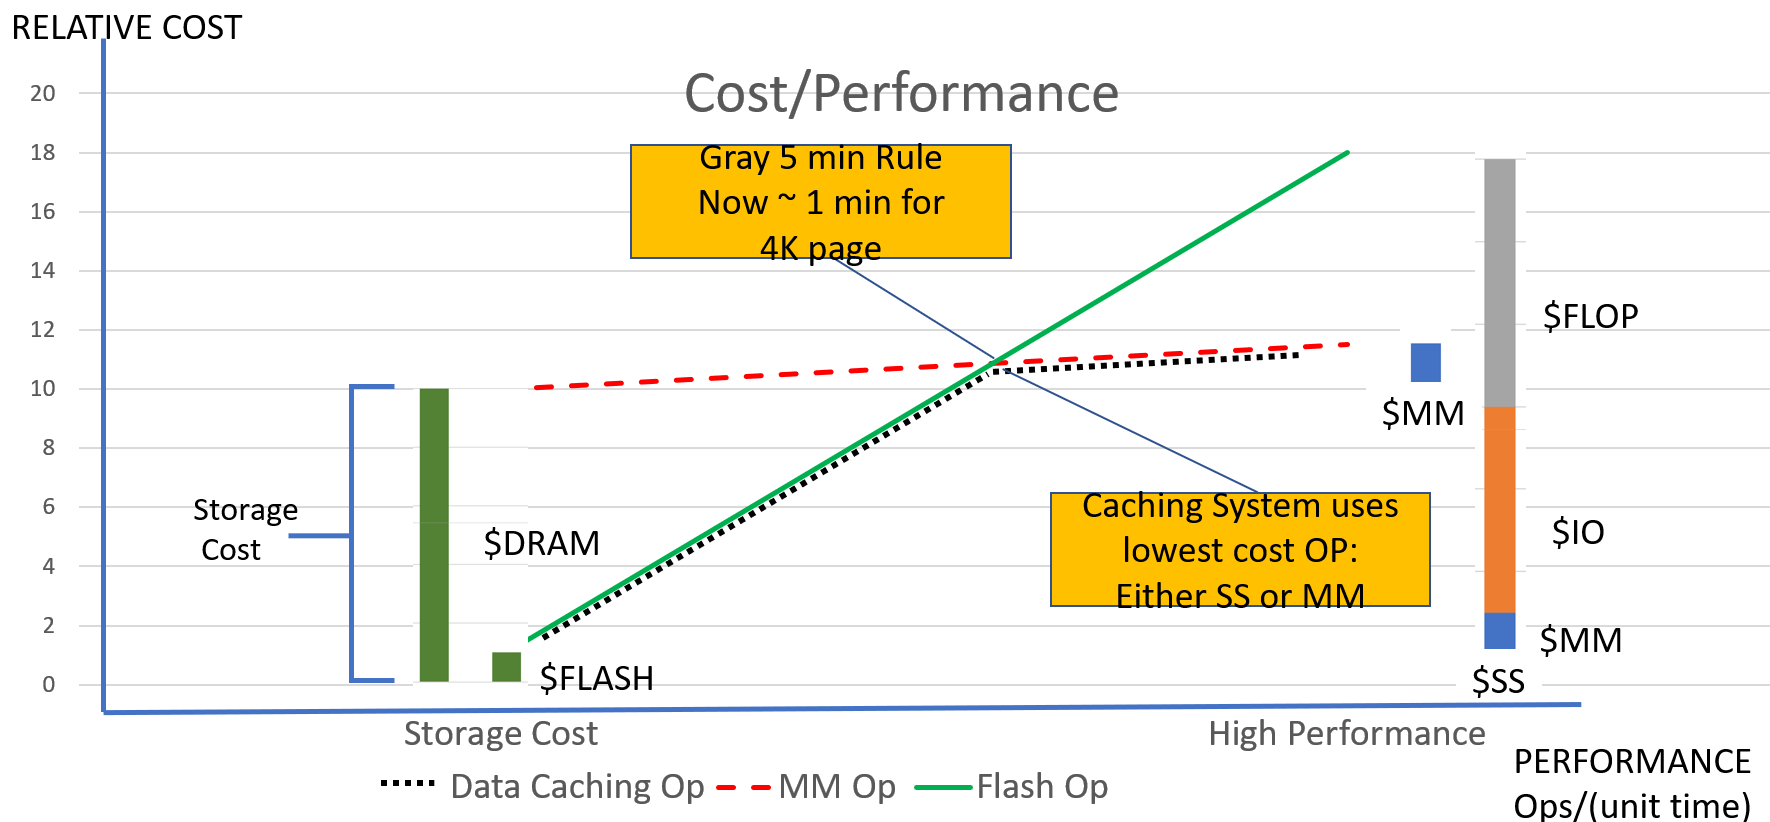
\includegraphics[height=1.5in]{breakeven.png}
\caption{The cost/sec of main memory operations and secondary storage operations as execution rates change.}
\label{fig:MMSS}
\end{figure}


At low access rates, the cost of storage dominates the execution cost.  Since main memory is $10X$ more costly than flash, an $MM$ operation is $11X$ more expensive than an $SS$ operation at very low access rates.  At high access rates, it is the execution cost that dominates.  \$SOP is about $12X$ the cost of \$MOP, with \$FLOP approximately $6X$ of \$MOP, and \$IO about $5X$ of \$MOP.  The number of IOPS provide by an SSD has dramatically increased, reducing \$FLOP. Thus CPU cost (\$IO) for an I/O is now a significant part of \$SOP cost. 


Trading space (cost) for time (cost) can be useful for improving systems, but how much space for how much performance?  We analysed other technologies in~\cite{Damon} which showed similar cross-over points frequently exist where relative cost advantage also changes between systems.  Using more main memory, as done by the main memory MassTree key-value store results in its performance being higher than Deuteronomy's.  In our experiments, the breakeven point for a page at about $T_i = 3$ seconds.  Hence MassTree is better for very hot data, but not for data accessed less frequently.  Data compression saves storage cost at the expense of increasing execution cost, hence good for very cold data, even though decompression adds to execution cost.  

\vspace{-.1cm}
\section{Concluding Thoughts}

Cost/performance is usually more important than sheer performance.  And storage costs are a very big part of overall costs, since most data is cold.  Further, the hot data set typically changes over time.  Cost effective data management means reducing storage costs for cold data and reducing execution cost for hot data.  That is what data caching systems do. Data caching systems dominate the market via better cost/performance, despite main memory systems having higher performance.  

There is another message here.  Research may dramatically increase data caching system performance.  For example, reducing the cost of moving data between storage hierarchy levels could be a huge win, enabling new and cheaper storage technologies to play an important role in data management.  That research agenda might succeed in producing a "one size" system that fits (almost) all~\cite{onesizefitsall} of the data management market.



\vspace{-.1cm}
\section{Acknowledgements}
I want to thank Haixun Wang for inviting me to write this opinion piece.  Thanks also to my Deuteronomy colleagues, particularly Justin Levandoski, Sudipta Sengupta, and Ryan Stutsman.  Together, we built a great data caching system.

%\newpage
\vspace{-.1cm}
\bibliographystyle{ACM-Reference-Format}
\begin{thebibliography}{10}
\begin{small}



\itemsep=-.5pt


\bibitem{diaconu}
C. Diaconu, C. Freedman, E. Ismert, P. Larson, P. Mittal, R. Stonecipher, N. Verma, M. Zwilling:
Hekaton: SQL server's memory-optimized OLTP engine. SIGMOD 2013: 1243-1254



\bibitem{gray1}
J. Gray, G. R. Putzolu:
The 5 Minute Rule for Trading Memory for Disk Accesses and The 10 Byte Rule for Trading Memory for CPU Time. SIGMOD 1987: 395-398


\bibitem{hyper13}
A. Kemper, T. Neumann, J. Finis, F. Funke, V. Leis, H. M\"{u}lhe, T. M\"{u}hhlbauer, W. R\"{o}diger:
Processing in the Hybrid OLTP \& OLAP Main-Memory Database System HyPer. IEEE Data Eng. Bull. 36(2): 41-47 (2013)


\bibitem{LLS13}
J. Levandoski, D. Lomet, and S. Sengupta,
The Bw-Tree: A B-tree for New Hardware Platforms,
ICDE 2013, pp. 302--313.

\bibitem{LLS13a}
J. Levandoski, D. Lomet, S. Sengupta.
LLAMA: A Cache/Storage Subsystem for Modern Hardware.
PVLDB 6(10): 877-888 (2013).

\bibitem{TC}
J. Levandoski, D. Lomet, S. Sengupta, R. Stutsman, R. Wang:
High Performance Transactions in Deuteronomy.
CIDR 2015.

\bibitem{Damon}
D. Lomet: Cost/performance in modern data stores: how data caching systems succeed. DaMoN 2018: 9:1-9:10

\bibitem{rocksdb}
RocksDB: A persistent key-value store for fast storage environments.
\url{http://rocksdb.org/}

\bibitem{onesizefitsall}
M. Stonebraker, U. Cetintemel, ``One size fits all": an idea whose time has come and gone. ICDE 2005.


\bibitem{voltdb}
M. Stonebraker, A. Weisberg:
The VoltDB Main Memory DBMS. IEEE Data Eng. Bull. 36(2): 21-27 (2013)



\end{small}
\end{thebibliography}


\end{document}

\end{opinion}
\begin{opinion}{The Ubiquity of Subjectivity}
{Alon Halevy}{}
\documentclass[11pt]{article}

\usepackage{wrapfig}
\usepackage{setspace,lipsum}

\usepackage{deauthor,times,graphicx}
\usepackage{color}
\usepackage{eurosym}
\newcommand{\biggorilla}{\mbox{\sc BigGorilla}}
\newcommand{\koko}{\mbox{\sc Koko}}
\newcommand{\flexmatcher}{\mbox{\sc FlexMatcher}}
\newcommand{\magellan}{\mbox{\sc Magellan}}

\newcommand{\tanedit}[1]{{\small \color{blue}~#1}}
\newcommand{\alonedit}[1]{{\small \color{blue}#1}}
\newcommand{\anhaiedit}[1]{{\small \color{blue}#1}}
\newcommand{\spanstr}[1]{{``{\em\small #1}''}}
\newcommand{\token}[1]{\mbox{\rm #1}}
\newcommand{\pystr}{\mbox{\sc py\_stringmatching}}
\newcommand{\pyssj}{\mbox{\sc py\_stringsimjoin}}
\newcommand{\mg}{\mbox{\sc Magellan}}
\newcommand{\where}{\mbox{\sf where}}
\newcommand{\extract}{\mbox{\sf extract}}
\newcommand{\similarTo}{\mbox{\sf similarTo}}
\newcommand{\from}{\mbox{\sf from}}
\newcommand{\ifclause}{\mbox{\sf if}}
\newcommand{\satisfying}{\mbox{\sf satisfying}}
\newcommand{\withthreshold}{\mbox{\sf with threshold}}
\newcommand{\eqclause}{\mbox{\sf eq}}
\newcommand{\inclause}{\mbox{\sf in}}
\newcommand{\orclause}{\mbox{\sf or}}
\newcommand{\excluding}{\mbox{\sf excluding}}
\newcommand{\near}{\mbox{\sf near}}
\newcommand{\contains}{\mbox{\sf contains}}
\newcommand{\mentions}{\mbox{\sf mentions}}
\newcommand{\matches}{\mbox{\sf matches}}
\newcommand{\alt}{\mbox{\sf or}}
\newcommand{\desc}[1]{\{\mbox{\em #1}\}}
\newcommand{\posverb}{\mbox{\sc verb}}
\newcommand{\w}[1]{\mbox{\{{\em #1}\}}}
\newcommand{\descriptor}[1]{\mbox{$[[$#1$]]$}}
\newcommand{\dm}{\mbox{\sc DeepMatcher}}




%\author{ Alon Halevy}


\begin{document}
%\title{The Ubiquity of Subjectivity}
%\maketitle

\begin{abstract}
In order to make effective use of data in decision making, we need to consider aspects of data that our research community has traditionally ignored.  These include the management of subjective data, building unbiased presentations that are tailored to the subjective world-view of the recipient, and finally, the subjective nature of human decision making.
\end{abstract}

\section{Introduction}

Data has become an integral part of our lives. We use data to make a wide spectrum of decisions, such as what to wear today, where to go for dinner and on vacation,  which charity to support, and who to vote for in the elections. Ideally, we'd like to think that if we just had all the facts,  decisions would be easy and disagreements would be quickly settled. As a research community, our goal has been to fuel such decision making by  focusing on  extracting, managing, querying and visualizing data and facts.  I argue here that we need to acknowledge the subjective aspects of data and decision making and broaden our agenda to incorporate them into the systems we build.  

Subjectivity is prevalent in at least three levels. First, the data itself may be subjective: there is no ground truth about whether a restaurant is romantic or a travel destination is relaxing. We need to develop techniques to extract, manage and query subjective data. Second, presentation of the data can be subjective either by introducing bias (intentionally or not), or by tailoring the presentation to the frame of mind of the recipient. Third, human decision making is inherently subjective and based on emotions. We need to understand how to incorporate the emotional aspect of decision making into our systems.  

The following sections will expand on each of these topics.  I have already done some research on the first topic~\cite{subjectivedatabases} and so my comments will be more concrete. However, I believe all three areas are equally important.

\section{Subjective data}
When we compare between multiple options (e.g., hotels, restaurants, online courses), we typically lean on subjective data that describes the {\em experiential aspects} of these options. Today, this data resides in online reviews. For example, reviews will give insights on whether a restaurant has a quiet ambience,   
a hotel has helpful staff, or a school has good faculty. While today's online shopping sites make significant attempts at surfacing key quotes from reviews and even classifying them into several categories, a user cannot put these conditions in the query  (e.g., {\em hotels up to \$250 a night with helpful staff}). Hence, we end up sifting through many reviews until we get exhausted and settle for sub-optimal choices. 

Database systems traditionally focus on the {\em objective} attributes of entities (e.g., the price and location of a hotel, or the cuisine of a restaurant). One exception, which captures a narrow aspect of subjective data, is modeling reviewers' opinions as star ratings, and letting users query the aggregate ratings. 
Subjective data introduces additional technial challenges because it is expressed in free text, is very nuanced, and  does not lend itself to a clean schema.   
The Natural Language Processing  (NLP) community has spent significant effort on subjective data. That community investigated problems such as identifying subjective data~\cite{DBLP:journals/coling/WiebeWBBM04}, studying how subjectivity affects the meaning of words~\cite{DBLP:conf/acl/WiebeM06}, learning extraction patterns for it~\cite{DBLP:journals/taffco/WiebeR11}, and creating summaries of online reviews~\cite{liu2012sentiment}.   Management of subjective data presents an interesting opportunity to combine techniques from databases and NLP.

The first challenge involving subjective data is answering complex queries. 
Roughly speaking, from a query processing perspective, the NLP community has addressed the problem of retrieving individual facts (e.g., finding comments about the friendliness of the hotel staff).  However, to answer more complex queries, a system needs to be able to combine multiple query predicates and to aggregate opinions across many reviews. Combining multiple subjective predicates (e.g., {\em hotels with quiet rooms and friendly staff}) is similar in spirit to the problem of combining multiple sources of fuzzy information~\cite{fagin1996combining}.  
Aggregating subjective data is crucial because users typically want to get an overview of the reviews at hand. The problem of aggregating reviews is fascinating because it requires mapping textual expressions to some meaningful scale. 

The second challenge regarding subjective data is that the schema is much more fluid. Since experiential aspects of an entity can be extremely varied and nuanced, it's not clear which of them to include in the schema. Some attributes may be related to each other or mostly determined by others (e.g., {\sc friendlyStaff} and {\sc helpfulStaff}). Hence, a subjective database system cannot assume that every query it receives can be answered with its schema. In some cases, it will need to find attributes in the schema that are closest to the query terms. In other cases, when the system has low confidence that the schema can be used to answer the query, it will need to fall back on the actual text in the reviews. In some ways, this challenge is similar to how web search engines straddle the boundary between structured and unstructured data.  When a search engine can confidently map a query to an entity in their knowledge graph, the engine presents a knowledge card with structured data.  When the engine thinks the answer appears in a paragraph or an HTML table on the Web, they present that result prominently. But when both of these fail, they fall back on links to ranked Web pages.  


Finally, at the core of the subjective evaluation of data is also the subjective view of the user asking the query.
A hotel that would be considered clean for one person may not cut it for another, and obviously the same goes for cafes. 
Hence, when  user profiles are available, a subjective database should tailor its answers to the user.
 User profiles may be collected passively from previous queries, clicks or purchases, or they may be constructed by answering a few survey questions.
 The next two sections dive deeper into the topic of the user perception. 

\section{Subjective presentation}
To be useful in decision making, data needs to be communicated to a user either textually, orally or visually.  There are two dimensions to subjectivity in the presentation: {\em faithfulness}--whether the data is presented  without bias, and {\em effectiveness}--whether the data is presented in a way that is likely to resonate with the frame of mind of the recipient.

In terms of faithfulness, there are several common methods to create a misleading presentation, including 
 omission, alluding to the {\em straight-line instinct}, and improper comparison~\cite{factfulness}. An example of omission is in Figure~\ref{fig:fig}(a) showing that unemployment rates in the US have been going down since Donald Trump took office in January, 2017, whereas Figure~\ref{fig:fig}(b)  shows that it is merely a continuation of the trend that began during the previous administration. An example of alluding to the straight-line instinct would be to show the world population growth graph in Figure~\ref{fig:fig}(c) and letting the readers extrapolate that it will grow indefinitely. In fact, the common estimates show that the world population will actually peak around 2050. An example of improper comparison would be to state that the GDP of the USA grew by 2.3\% in 2017 but without presenting growth numbers for comparable economies. Note that in some cases search engines already show comparable points when presenting structured data. 

\begin{figure}
\subfloat[a]{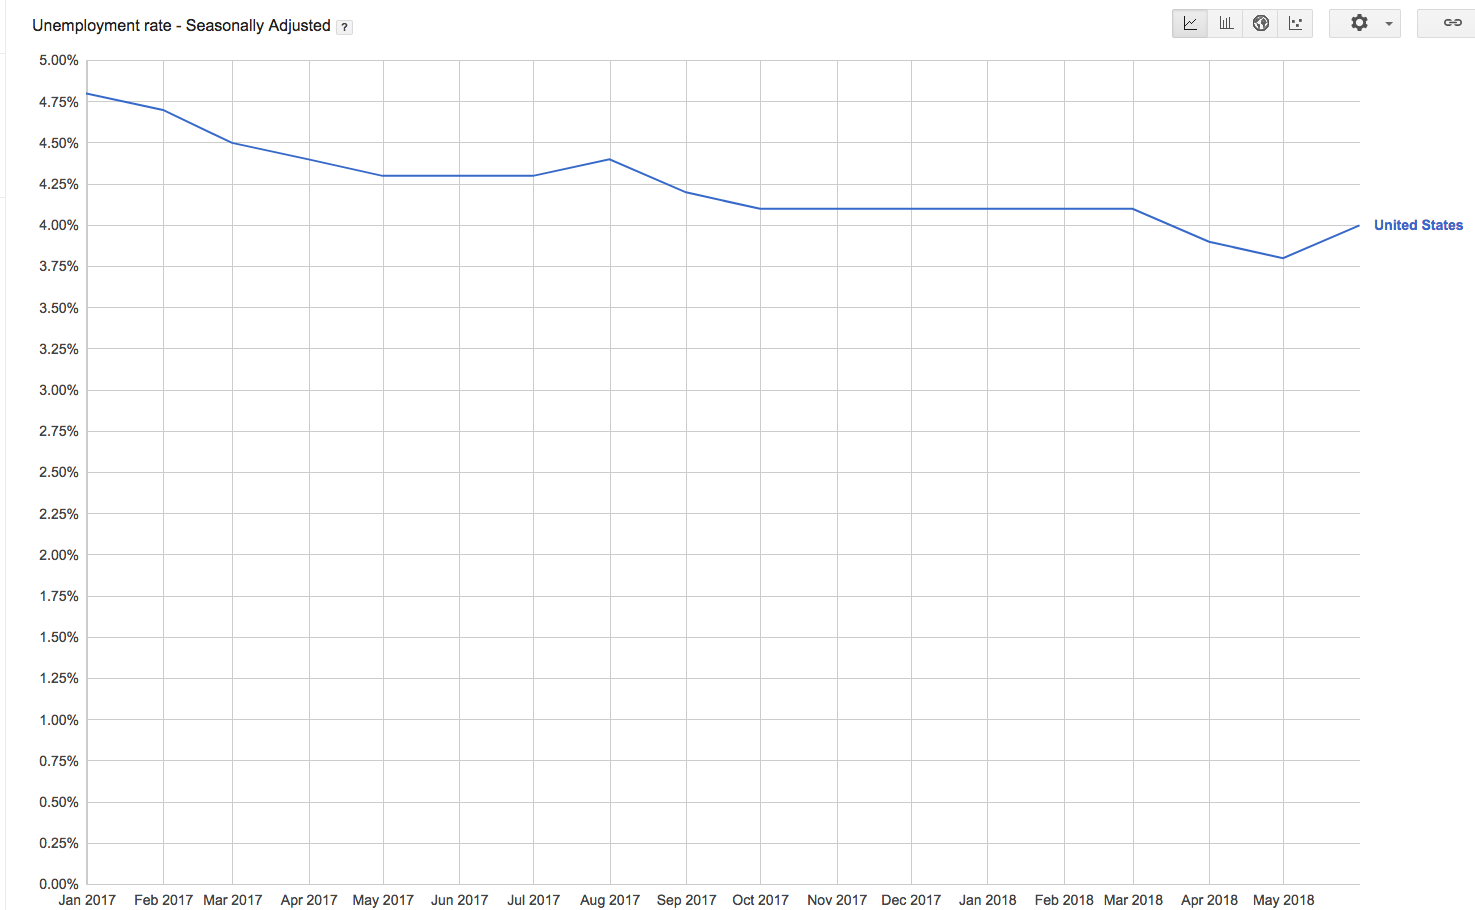
\includegraphics[width = 1.7in]{letters/unemp2017.png}}
\subfloat[b]{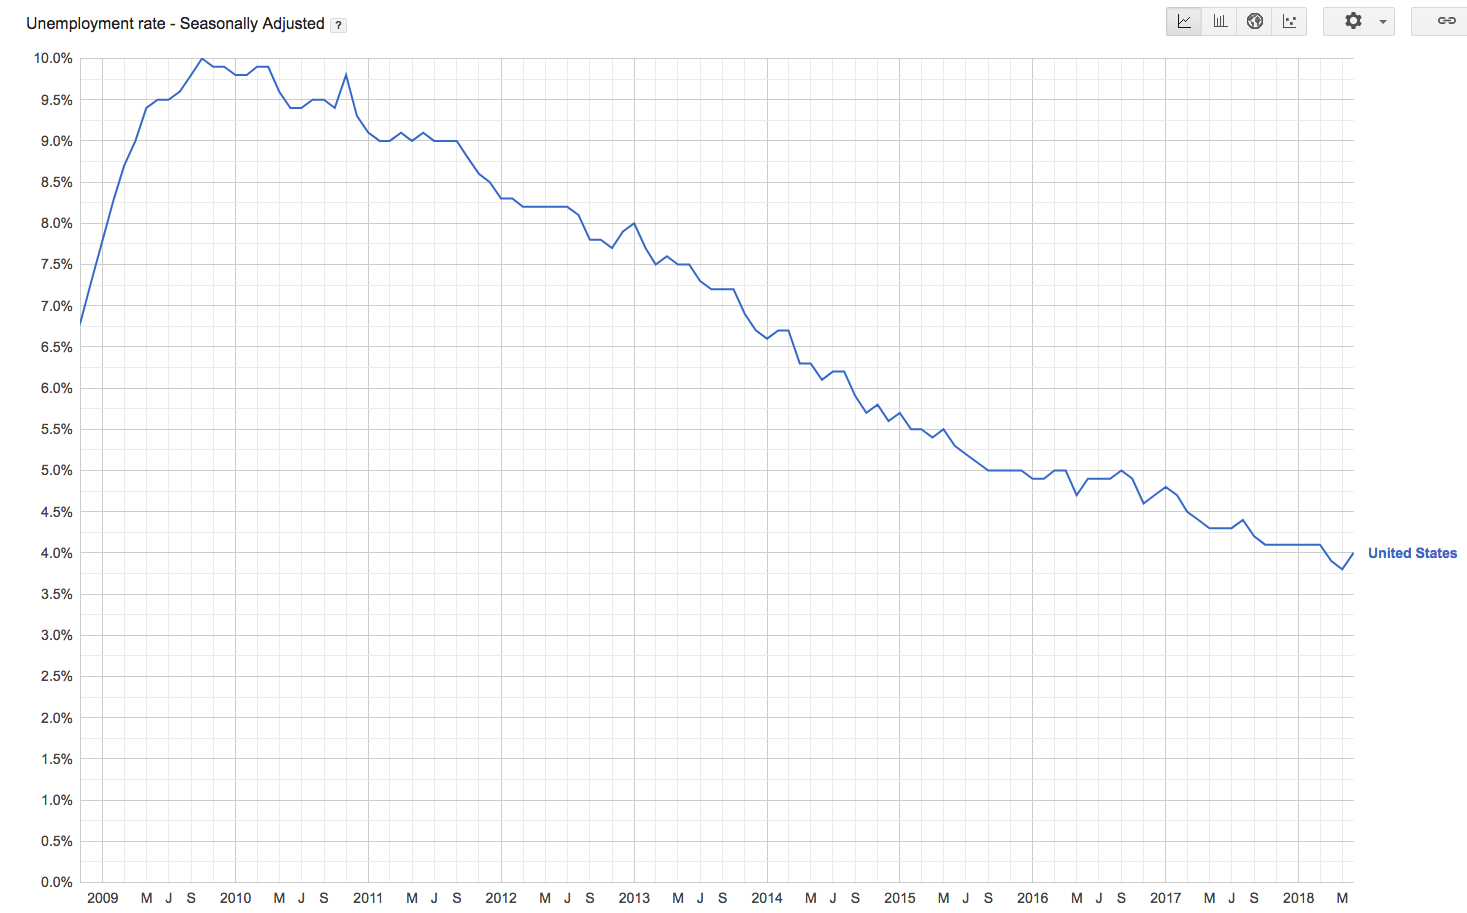
\includegraphics[width = 1.7in]{letters/unemp2009.png}}
\subfloat[c]{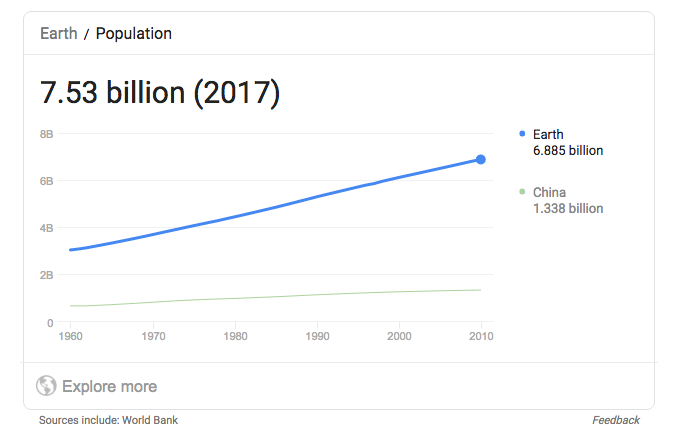
\includegraphics[width = 1.7in]{letters/worldpop.png}} 

\caption{(a) is the unemployment rate in the USA since 2017 and (b) is the rate since 2009. (c) is the world population over time.}
\label{fig:fig}
\end{figure}

In the above examples the presenter seems at least slightly nefarious by hiding relevant aspects of the data (see~\cite{DBLP:conf/edbt/StoyanovichAM16} for a more detailed discussion of fairness in data analysis). But subjectivity in presentation can also be done in trying to frame data in a way that can resonate better with the recipient. Such a presentation could make the difference between making a convincing case or falling on flat ears. Lakoff and Wehling discuss the framing issue  in the context of political debates~\cite{lakoff-book}. They discuss the example of the healthcare debate in American politics and claim that once the healthcare is framed as a product, there is little chance of convincing conservatives that it should be available to everyone and that everyone should be forced to buy healthcare. After all, a government should not force its citizens to buy {\em any} product, be it peanut butter, striped socks, or healthcare? In contrast, if healthcare is framed as an issue of freedom, which is central to the conservative doctrine, then conservatives would see the merits. After all, you are not truly free if a medical condition can completely deplete all your assets.   

The above discussion leads to several research problems: 
(1) {\em is $P$ a faithful presentation of the data $D$?} (2) {\em Does a presentation $P$ of data $D$ support an argument $A$}?  (3) {\em is the presentation $P$ of data $D$ effective for the user $U$?} Note that effectiveness is different from relevance--data can be relevant, but the user may still ignore it if not presented effectively. In a particular context, these problems will be made more specific. For example, we will have some space of possible presentations (e.g., graphs spanning different time periods), and for elements of that space we can consider specific questions, such as would a presentation of a graph of a variable over time incorrectly lead to inducing wrong conclusions with the straight line instinct? Could one falsely conclude a particular pattern without looking at a broader time scale?  What are appropriate comparison points for a particular datum? 

\section{Subjective decision making}
We would like to think that our decision making is rational and based on hard facts. In practice, however, it is well known from psychology and Neuroscience that our emotions, which express many of our subjective preferences, play a large part in our decision making~\cite{kahneman}. In fact, it has been shown that {\em without} emotions we cannot make even simple decisions. A famous case in point was Antonio Damasio's patient named Elliot~\cite{damasio}. Elliot suffered a particular type of damage to his brain following the removal of a tumor and was unable to feel any emotion, even when he was shown very disturbing images. While Elliot's IQ remained in tact, he was not able to make simple decisions such as how to prioritize work items or choose an item from a restaurant menu.


I am not suggesting that the intricacies of decision making can be reformulated as a data management problem, but I think we can do a much better job at incorporating the emotional aspect of decision making into the systems we build.\footnote{Rosalind Picard already pointed in this direction in 1997 in her original book on Affective Computing~\cite{picard-book}, (page 220).} 
From a computational perspective, decision making involves exploring a large state space of possible outcomes, such as choosing a hotel to stay during a trip, or the best method for securing child care for your baby. The first challenge to decision making arises because the number of possible states may be too large to consider,  especially under time and attention pressure. Second, we may have incomplete or only probabilistic knowledge about these possible states, making the comparison even sketchier. Finally, many of the choices we make in life (e.g., between job offers or romantic prospects) are not really directly comparable  to each other.

To reach decisions effectively, we prune the search space using heuristics that may not be conscious (e.g., certain attributes of entities end up being more important under certain conditions). Developing an understanding of how we prune the decision search space and methods that result in better decisions presents an exciting area of research that our current data science tool set is well poised to investigate.

\section{Conclusion}
To  realize the full potential of the vast amounts of data available to us today, systems need to be able to manage subjective data and to understand how prospective consumers of the data think and make decisions subjectively. I've tried to outline a few concrete steps on this research agenda. Of course, as we tackle these problems, we should also keep in mind that ultimately the data we have is merely an abstraction of the world and there will be other factors that are not included in the data that will influence our decisions and actions. In a nutshell, this is a call to consider concepts from psychology, behavior economics and neuroscience in the design of tools that enable decision making based on data. 

\section{Acknowledgements}
I'd like to thank my colleagues at Megagon Labs for inspiring many of the ideas described above: Wang-Chiew Tan, Vivian Li, Adi Zief-Balteriski, Yuliang Li and Jingfeng Li. Thanks to Phil Bernstein,  Anna-Lisa Gentile, Rada Mihalcea and Haixun Wang for several discussions relating to the topics covered.


%\scriptsize
%\newpage
\vspace{-.1cm}
\bibliographystyle{ACM-Reference-Format}
\begin{thebibliography}{10}
\begin{small}



\itemsep=-.5pt

\bibitem{damasio}
A.~Damasio.
\newblock {\em Descartes' Error}.
\newblock Springer, 1994.

\bibitem{fagin1996combining}
R.~Fagin.
\newblock Combining fuzzy information from multiple systems.
\newblock In {\em PODS}, pages 216--226. ACM, 1996.

\bibitem{kahneman}
D.~Kahnnman.
\newblock {\em Thinking Fast and Slow}.
\newblock Penguin Books, 2012.

\bibitem{lakoff-book}
G.~Lakoff and E.~Wehling.
\newblock {\em The Little Blue Book: The Essential Guide to Thinking and
  Talking Democratic}.
\newblock Free Press, 2012.

\bibitem{subjectivedatabases}
Y.~Li, J.~Li, A.~Feng, V.~Li, W.-C. Tan, and A.~Halevy.
\newblock Subjective databases.
\newblock {\em arXiv preprint arXiv:1309.0238}, 2019.

\bibitem{liu2012sentiment}
B.~Liu.
\newblock {\em Sentiment Analysis and Opinion Mining}.
\newblock {Morgan & Claypool}, 2012.

\bibitem{picard-book}
R.~Picard.
\newblock {\em Affective Computing}.
\newblock The M.I.T Press, 1995.

\bibitem{factfulness}
H.~Rosling, O.~Rosling, and A.~R. Rönnlund.
\newblock {\em Factfulness: Ten Reasons We're Wrong About the World--and Why
  Things Are Better Than You Think}.
\newblock Flatiron Books, 2018.

\bibitem{DBLP:conf/edbt/StoyanovichAM16}
J.~Stoyanovich, S.~Abiteboul, and G.~Miklau.
\newblock Data responsibly: Fairness, neutrality and transparency in data
  analysis.
\newblock In E.~Pitoura, S.~Maabout, G.~Koutrika, A.~Marian, L.~Tanca,
  I.~Manolescu, and K.~Stefanidis, editors, {\em Proceedings of the 19th
  International Conference on Extending Database Technology, {EDBT} 2016,
  Bordeaux, France, March 15-16, 2016, Bordeaux, France, March 15-16, 2016.},
  pages 718--719. OpenProceedings.org, 2016.

\bibitem{DBLP:conf/acl/WiebeM06}
J.~Wiebe and R.~Mihalcea.
\newblock Word sense and subjectivity.
\newblock In N.~Calzolari, C.~Cardie, and P.~Isabelle, editors, {\em {ACL}
  2006, 21st International Conference on Computational Linguistics and 44th
  Annual Meeting of the Association for Computational Linguistics, Proceedings
  of the Conference, Sydney, Australia, 17-21 July 2006}. The Association for
  Computer Linguistics, 2006.

\bibitem{DBLP:journals/taffco/WiebeR11}
J.~Wiebe and E.~Riloff.
\newblock Finding mutual benefit between subjectivity analysis and information
  extraction.
\newblock {\em {IEEE} Trans. Affective Computing}, 2(4):175--191, 2011.

\bibitem{DBLP:journals/coling/WiebeWBBM04}
J.~Wiebe, T.~Wilson, R.~F. Bruce, M.~Bell, and M.~Martin.
\newblock Learning subjective language.
\newblock {\em Computational Linguistics}, 30(3):277--308, 2004.

\end{thebibliography}



\end{document}

\end{opinion}
\end{opinionsection}




\begin{articlesection}{Cross-Layer Support for Database Management}
%
%  Contributed articles section.  Use the articlesection environment.
%  Each article is contained in an article environment, where the two required
%  options to \begin{article} are the title and author of the article
% typically, an article is stored in a directory named with one of the author names, and is then "input" into the issue
%
\begin{article}
{From the Application to the CPU: Holistic Resource Management for Modern Database Management Systems}
{Stefan Noll, Norman May, Alexander B\"{o}hm, Jan M\"{u}hlig, Jens Teubner}
\graphicspath{{submissions/snoll/figs/}}
\documentclass[11pt]{article}

\usepackage{deauthor,times,graphicx}
%\graphicspath{{noll/}}

\usepackage{subfig}
\usepackage{listings}
\usepackage{hyperref}


%\graphicspath{{./}}










\begin{document}
\title{From the Application to the CPU: Holistic Resource Management for Modern Database Management Systems}
\author{%
{Stefan Noll{\small$~^{\#+*}$}, Norman May{\small$~^{\#}$}, Alexander B\"{o}hm{\small$~^{\#}$}, Jan M\"{u}hlig$~^{+}$, Jens Teubner{\small$~^{+*}$} }
\vspace{1.2mm}\\
\fontsize{10}{10}\selectfont\rmfamily\itshape
$^{\#}$\,SAP SE, Germany\\
\fontsize{9}{9}\selectfont\ttfamily\upshape
\{stefan.noll,norman.may,alexander.boehm\}@sap.com
\vspace{1.6mm}\\
\fontsize{10}{10}\selectfont\itshape
$^{+}$\,Databases and Information Systems Group, TU Dortmund University, Germany\\
\fontsize{9}{9}\selectfont\ttfamily\upshape
jan.muehlig@tu-dortmund.de\\
\fontsize{9}{9}\selectfont\ttfamily\upshape
jens.teubner@cs.tu-dortmund.de
\vspace{1.6mm}\\
\fontsize{10}{10}\selectfont\itshape
$^{*}$\,Informatik Centrum Dortmund e.V., Germany
}
\maketitle

\begin{abstract}
With their capability to perform both high-speed transactional processing and complex analytical workloads on the same dataset and at the same time, Operational Analytics Database Management Systems give enormous flexibility to application developers.
Particularly, they allow for the development of new classes of enterprise applications by giving analytical insights into operational data sets in real time.
From a database system point of view though, these applications are very demanding, as they exhibit a highly diverse combination of  different query workloads with inhomogeneous performance and latency requirements.
In this article, we discuss the practical implications and challenges for database architects and system designers. We propose solutions that---by sharing semantics between the application, the database system, the operating system, and the hardware---allow to manage complex and resource-intensive workloads in an efficient and holistic way.
\end{abstract}



\section{Introduction}
Driven by the idea of enabling both transactional processing as well as real-time analytical query workloads in the context of a single system~\cite{nollhrm19:Plattner:2009:ACA}, a new class of database management systems has emerged, referred to as operational analytics database management systems~\cite{nollhrm19:Boehm:2016:OAD}.
These systems envision to simplify the data management landscape by consolidating multiple, disparate use cases.
Consequently, they allow the creation of novel business applications which seamlessly combine both real-time analytics and transaction processing \cite{nollhrm19:Leukert:2015:TIR}.
From a database system designer's point of view, however, delivering high performance for these modern applications puts up additional challenges because their workload characteristics are highly diverse and demanding.

In particular, static workload management schemes and simple heuristics perform suboptimally considering end-to-end performance~\cite{nollhrm19:Wolf:2014:SUM}.
The reason for this is that even the same query can have different priorities from an application's point of view, depending on the context it is being executed in.
A simple primary-key based lookup operation can be issued, e.g, in the context of a \emph{mission-critical} and time-sensitive OLTP transaction such as the \emph{interactive} data entry by a business user, but also as part of a \emph{non-critical} batch transaction that runs for hours in the \emph{background}.
A complex analytical query can be sent in the context of, e.g., a \emph{scheduled} quarter-end close report (making it rather uncritical from an execution time point of view), but also as part of a \emph{user-driven}, interactive dashboard application where virtually every millisecond counts.

Motivated by these observations, we share the opinion of other researchers that individual hard- and software-solutions throughout the data processing stack fail to address the complex challenges of these systems in isolation~\cite{nollhrm19:Giceva:2013:COD, nollhrm19:Giceva:2017:COS}.
Particularly, we believe that they are best addressed by a holistic approach, and in collaboration between the application, database management system, and the underlying hardware~\cite{nollhrm19:Boehm:2015:NOT}.

\paragraph{Outline.}
This article is structured as follows.
In Section \ref{nollhrm19:sec:hana_wlm}, we discuss how to bridge the semantic gap between the application and the database system.
Communicating additional workload context information and priorities allows the database system to perform prioritization, scheduling, and resource management that is in line with the expectations of the application.
Next, Section \ref{nollhrm19:sec:cpu_cache_partitioning} discusses a similar technique which allows the database system to share semantic information about data access patterns with the underlying hardware (i.e., the processor) by using CPU cache partitioning.
This enables the more efficient utilization of CPU caches, specifically for heterogeneous, highly concurrent workloads.
In Section \ref{nollhrm19:sec:dbms_os}, we highlight different approaches for database management systems to interact with the operating system, e.g., to improve scaling and robustness.
While commercial database systems usually choose to circumvent the OS exploiting detailed workload information, another strategy is bringing the database system and the operating system closer together with a radical co-design.
We conclude the article in Section \ref{nollhrm19:sec:conclusion}.



\section{Workload Management in SAP HANA}
\label{nollhrm19:sec:hana_wlm}

Analytical and transactional workloads do not only have different resource demands, they are also linked to different performance expectations.
\emph{Transactional} workloads are characterized by operations which consume relatively little memory and compute power.
However, they are usually sensitive to lock contention.
Unfortunately, this resource contention leads to fluctuations in statement response times, while applications expect predictable throughput and response time characteristics.
In our experience, customers are willing to sacrifice peak performance in return for better predictability of statement response times.
\emph{Analytical} workloads, on the other hand, typically are demanding regarding CPU and memory consumption.
In particular, single analytical ad-hoc statements may consume excessive amounts of memory or CPU.
This is particularly problematic for operational analytics DBMS when demanding analytical statements take away CPU clock cycles and slow down concurrent transactional workloads~\cite{nollhrm19:Wolf:2014:SUM}.

To balance or prioritize different workloads and to comply with a \emph{service level agreement} (SLA), commercial DBMS usually employ \emph{workload management} to manage resources available to single statements, applications or database users, see~\cite{nollhrm19:Zhang:AWLM:2014} for a good overview.
In SAP HANA, workload management works on a fine-grained level~\cite{nollhrm19:HANA:2018:AdminGuide} because the system is optimized for modern multi-core architectures with extensive multi-threading~\cite{nollhrm19:Psaroudakis:2015:SUC:2824032.2824043}.
Limiting, e.g., the number of working threads or the amount of memory available to the engine, can be managed for entire workloads or individual statements.
While this creates a powerful tuning option for the user, the system has to track and enforce resource consumption in all of its components.
In the following, we briefly present two mechanisms for implementing workload management using the example of SAP HANA: \emph{workload classes} and \emph{admission control}.

\paragraph{Workload Classes.}
In SAP HANA \emph{workload classes} address 1) the requirement of avoiding the excessive resource consumption of single statements and 2) the requirement of isolating the resource demands of different applications, database users, etc.\@
Workload classes are containers of configuration parameters like priority, query timeout, limits of memory consumption, or limits of concurrency per statement or per group of statements.
They are defined in the database catalog and can be applied to all statements of a database connection.
Workload classes depend on context information passed by the client application: session variables, key-value pairs maintained per database connection, e.g., \texttt{APPLICATION="ETL"}.
This context information is matched to a \emph{workload mapping} which defines the set of session variables to consider and the mapping to a workload class.

The example in Listing~\ref{nollhrm19:lst:workload_classes} defines a workload class \texttt{ETLWorkloadClass}.
Statements executed in the context of this workload class may not consume more than $5\,\mathrm{GB}$ of memory and will not use more than one thread.
The corresponding workload mapping \texttt{ETLWorkloadMapping} will apply this workload class if the session variable \texttt{APPLICATION="ETL"} is set in the database connection.
We have confirmed in many customer scenarios that workload classes can significantly help to achieve high performance and robust system behavior.

\begin{lstlisting}[
caption={Simple example of using workload classes in SAP HANA.},
captionpos=b,
label=nollhrm19:lst:workload_classes,
language=SQL,
basicstyle=\ttfamily,
]
CREATE WORKLOAD CLASS "ETLWorkloadClass"
   SET 'STATEMENT MEMORY LIMIT' = '5',
       'STATEMENT THREAD LIMIT' = '1';

CREATE WORKLOAD MAPPING "ETLWorkloadMapping"
       WORKLOAD CLASS "ETLWorkloadClass"
   SET 'APPLICATION NAME' = 'ETL'; 
\end{lstlisting}

\paragraph*{Experimental Results.}
\begin{figure}
\centering
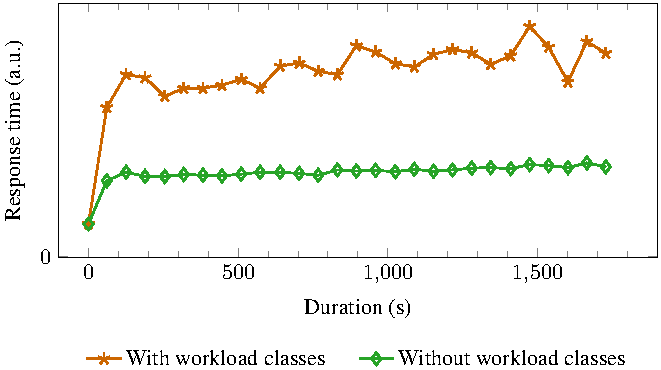
\includegraphics[bb=0 0 317 178]{figure1.pdf}
\caption{Average response time of web requests with and without using workload classes.}
\label{nollhrm19:plt:wlm_jmeter}
\end{figure}
Figure~\ref{nollhrm19:plt:wlm_jmeter} illustrates how workload classes can improve response time of web requests in peak load situations.
We measure the average response time per web request: 
Using JMeter we issue continuously 50 web requests per second.
In addition, we slowly increase analytical and ETL load by adding five queries to each workload every five minutes.
Eventually, we reach a very high system load with close to $100\,\mathrm{\%}$ CPU utilization.
Using workload classes, we limit the ETL and the analytical workload to one thread and $5\,\mathrm{GB}$ of main memory per SQL query (cf. Listing~\ref{nollhrm19:lst:workload_classes}).
Thus, the ETL and analytical load is handled using a best-effort strategy with reduced resource usage.
The results demonstrate that enabling workload class management keeps the average response time of the web requests at a low, predictable value.

\begin{figure}
\centering
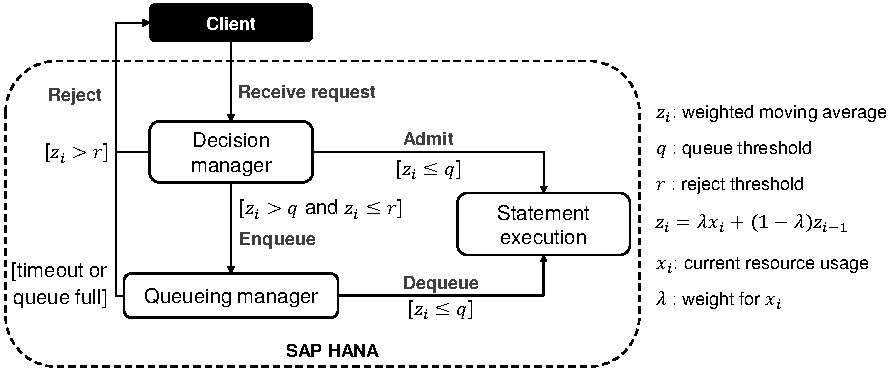
\includegraphics[bb=0 0 427 178]{figure2.pdf}
\caption{Request processing in SAP HANA using admission control.}
\label{nollhrm19:fig:hana_admission_control}
\end{figure}

\paragraph{Admission Control.}
Workload classes influence the resource consumption during execution when a statement was already admitted by the database processes.
However, a reasonably sized system may still experience short peaks in CPU or memory consumption that may result in contention of memory, CPU or latches.
Hence, in SAP HANA we complement workload classes with an \emph{admission control} mechanism.
A schematic overview is depicted in Figure~\ref{nollhrm19:fig:hana_admission_control}.

The admission control mechanism maintains a weighted moving average $z_i$ for all monitored resources of the host such as CPU utilization or total memory consumption.
When SAP HANA receives a new database request, it checks the weighted moving average against thresholds for each resource.
If each $z_i$ is below its corresponding queuing threshold $q$, the statement is admitted for immediate execution.
If the statement cannot be executed immediately, each $z_i$ is checked against its corresponding reject threshold $r$.
If the resource usage is below the reject threshold, the statement is queued; otherwise it is rejected immediately.
SAP HANA periodically checks if the resource consumption has decreased below the queuing threshold.
When this is the case, a batch of requests is fetched from the queue and scheduled for execution.
Database requests may also be rejected when the queue exceeds a configurable size or when the request is queued for too long.

Admission control samples the current resource usage $x_i$ every second.
The value $x_i$ is taken into account with, e.g., a weight of $\lambda = 0.7$.
Note that the sampling interval in combination with the weighted moving average lessens the impact of peak load situations, while the thresholds assure that the system reaches a high load without being overloaded.
In addition, admission control assumes that the client application implements a reasonable strategy to retry rejected database requests.
We could verify in productive setups that admission control helps to avoid contention issues in peak load situations, and that customers profit from a more robust system behavior.

\paragraph*{Conclusion.}
Different workloads have different resource demands and performance characteristics.
To manage hardware resources efficiently or to comply with SLAs of various workloads, commercial systems employ \emph{workload management}.
Using SAP HANA as an example, we present two techniques.
\emph{Workload classes} limit, e.g., the amount of memory or number of threads for an entire workload or an individual statement by enforcing limits across all components of the DBMS.
In addition, \emph{admission control} manages incoming request before they are admitted into the system, monitors CPU and memory consumption, and ultimately accepts or rejects a request to improve response times in peak load scenarios.



\section{CPU Cache Partitioning}
\label{nollhrm19:sec:cpu_cache_partitioning}

Modern microprocessors feature a sophisticated hierarchy of caches to hide the latency of memory access.
However, multiple cores within a processor usually share the same last-level cache (LLC).
We observed that this can hurt performance and predictability, especially in concurrent workloads whenever a query suffers from cache pollution caused by another query running on the same processor: the throughput of cache-sensitive operators may degrade by more than $50\,\mathrm{\%}$~\cite{nollhrm19:Noll:2018}.
In particular, some workloads are highly sensitive to the available amount of CPU cache (e.g., random accesses to a small hash table), contrary to cache-insensitive operations such as a sequential scan of a large memory area.
The good news is that hardware manufacturers allow fine-grained control of cache allocation by offering mechanisms such as Intel's \emph{Cache Allocation Technology} (CAT) \cite{nollhrm19:Intel:2015:CAT:whitepaper}.
By integrating a cache partitioning mechanism, which partitions the cache for individual database operators, into the execution engine of a prototype version of SAP HANA, we were able to improve the overall system performance by up to $38\,\mathrm{\%}$.

\paragraph*{Cache-Sensitivity.}
We analyzed the cache-sensitivity of individual operators using the example of the \emph{column scan} operator, the \emph{aggregation with grouping} operator and the \emph{foreign key join} operator. 
Our results show that \emph{column scans} do not profit from a large LLC.
This observation does not come as a surprise because, by nature, scans read data exactly once from DRAM without re-using it.
\emph{Aggregations}, by contrast, can be highly sensitive to the size of the LLC.
The algorithm that we consider is based on hashing, and is most cache-sensitive whenever the size of the hash tables is comparable to the (configured) LLC size.
Only if the hash table is either very small or very large, cache sensitivity becomes less significant.
Finally, the cache sensitivity of \emph{foreign key joins} heavily depends on the input data, i.e., the cardinality of the primary keys:
If the size of the bit vector used internally is comparable to the size of the cache, the algorithm becomes cache-sensitive.
Otherwise the operator does not profit from a large LLC.

\paragraph*{Cache Partitioning.}
Traditionally, the user has little control over the cache, as it is entirely managed by hardware.
Techniques such as \emph{page coloring}~\cite{nollhrm19:Lee:2009:MMC:1687627.1687670} offer the possibility of partitioning the cache by allocating memory in specific memory pages, known to map to a specific portion of the cache.
But those techniques require significant changes to the OS and the application.
Plus, re-partitioning the cache at runtime requires copying the data~\cite{nollhrm19:4658653, nollhrm19:Zhang:2009:TPP:1519065.1519076}.

\begin{figure}
\centering
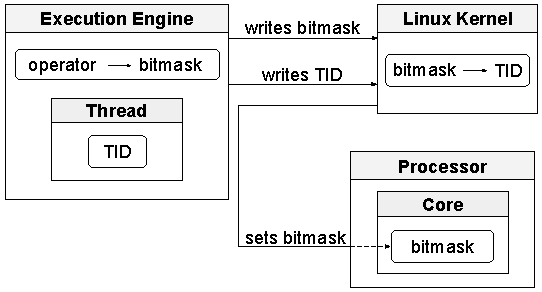
\includegraphics[bb=0 0 260 140]{figure3.pdf}
\caption{Interaction between the execution engine of SAP HANA, the Linux kernel and the processor.}
\label{nollhrm19:fig:hana_cat}
\end{figure}

With the microarchitecture codenamed ``Haswell'' Intel introduced \emph{Cache Allocation Technology} (CAT) \cite{nollhrm19:Intel:2015:CAT:whitepaper} to partition the \emph{last-level cache} of a processor.
We use the Linux kernel interface of CAT (available since version 4.10~\cite{nollhrm19:Intel:2017:CAT:Kernel}) to integrate cache partitioning into the execution engine of a prototype version of SAP HANA\@.
A schematic overview of how we retrofitted cache partitioning into an execution engine is illustrated in Figure \ref{nollhrm19:fig:hana_cat}.

The execution engine of SAP HANA uses a thread pool of worker threads to execute \emph{jobs}~\cite{nollhrm19:Psaroudakis:2015:SUC:2824032.2824043}, e.g., an operator.
We annotate a job with information of its \emph{cache usage}.
The approach is similar to \emph{workload classes}, but its granularity differs.
While \emph{workload classes} annotate entire queries, the cache partitioning mechanism annotates jobs, internal units of work often featuring a distinctive memory access pattern.
Currently, we distinguish between three categories of jobs:
\textit{(i)} jobs which are not cache-sensitive and pollute the cache such as the \emph{column scan};
\textit{(ii)} jobs which are cache-sensitive and profit from the entire cache such as the \emph{aggregation with grouping} operator for most cases; and
\textit{(iii)} jobs such as the \emph{foreign key join} operator which can be both cache-polluting and cache-sensitive depending on the query or data.
By default, a job belongs to \textit{(ii)} to avoid regressions.
During the execution of a job, the engine maps a job to a bitmask and passes the bitmask and the TID of the worker thread to the Linux kernel.
The Linux kernel associates the bitmask with the TID allowing it to update a core's bitmask during thread scheduling.
Integrating cache partitioning into the code base of an industry-strength system, described into more detail in~\cite{nollhrm19:Noll:2018}, requires only a small effort: our actual implementation consists of less than 1000 lines of code.

While we derived the cache partitioning scheme from an experimental analysis, the application of existing characterization methods for \emph{describing} the cache usage pattern of a database operator could be investigated.
For instance, Chou and DeWitt~\cite{nollhrm19:Chou:1985:EBM:1286760.1286772} propose the query locality set model based on the knowledge of various patterns of queries to allocate buffer pool memory efficiently.
Others propose the cache miss ratio as an online model for characterizing workloads or operators~\cite{nollhrm19:Tam:2009:RAL:1508244.1508259, nollhrm19:Manegold:2002:GDC:1287369.1287387, nollhrm19:Zhou:2004:DTP:1024393.1024415}.

\paragraph*{Experimental Results.}
Figure~\ref{nollhrm19:plt:scan_aggregate} illustrates some of our experimental results.
Our evaluation confirms that, e.g., \emph{aggregations} are sensitive to \emph{cache pollution} caused by, e.g., \emph{column scans}.
Aggregations are most sensitive to cache pollution whenever the size of their performance-critical data structures is comparable to the size of the LLC (cf. Figure~\ref{nollhrm19:plt:scan_aggregate}b).
Note that columns in SAP HANA are dictionary-compressed.
A compressed column contains indexes which reference values in a dictionary.
A dictionary is a sorted, unique sequence of the actual domain values.
Because the \emph{aggregation} operator decompresses its input to compute the aggregate, it performs many random accesses to the dictionary of the aggregated column.
Moreover, \emph{aggregations} frequently access hash tables used for grouping.

We observed that the throughput of the \emph{aggregation} query may drop below $60\,\mathrm{\%}$ compared to running isolated in the system.
By utilizing cache partitioning and restricting the \emph{column scan} to $10\,\mathrm{\%}$ of the available LLC, we can improve the throughput of the \emph{aggregation} query by up to $21\,\mathrm{\%}$.
In addition, the \emph{column scan} operator profits from the fact that the \emph{aggregation} operator consumes less memory bandwidth:
The throughput of the \emph{column scan} increases slightly by up to $6\,\mathrm{\%}$, too.
We determine that the overall cache hit ratio increases and that the LLC misses per instruction decrease because the \emph{aggregation} performs fewer accesses to main memory and more accesses to the cache.

While the \emph{column scan} operator always pollutes the cache, other operators such as the \emph{join} operator (not shown here) only cause cache pollution whenever its frequently accessed data structures fit in the L1 or L2 cache~\cite{nollhrm19:Noll:2018}.
In these cases, we can eliminate cache pollution as well and significantly improve performance by restricting the \emph{join} to a small portion of the LLC.
Generally, the search for the ``best'' partitioning in any given situation will depend on accurate \emph{result size estimates}.

\begin{figure}
\centering
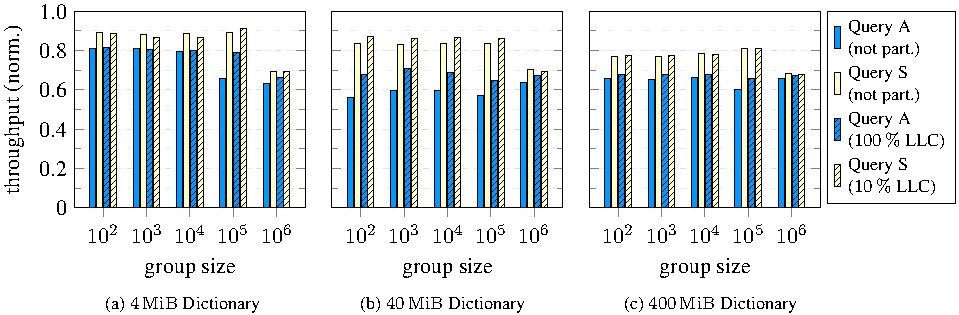
\includegraphics[bb=0 0 460 151]{figure4.pdf}
\caption{%
Throughput of Query~A (\emph{aggregation with grouping}) and Query~S (\emph{column scan}) when executed concurrently (normalized to their throughput when running isolated).
We vary the size of the dictionary of the aggregated column, we vary the number of groups, and we
disable or enable cache partitioning.
}
\label{nollhrm19:plt:scan_aggregate}
\end{figure}

\paragraph{Conclusion.}
In-memory database operators exhibit different performance characteristics depending on the available cache size.
We demonstrate how to integrate a cache partitioning mechanism into the execution engine of an existing DBMS with low expenditure and show in our evaluation that our approach avoids cache pollution and significantly reduces cache misses improving overall system performance.
Ultimately, our results illustrate that integrating cache partitioning into a DBMS engine is worth the effort: it may improve but never degrades performance for arbitrary workloads containing scan-intensive, cache-polluting operators.



\section{Interaction with the OS}
\label{nollhrm19:sec:dbms_os}

The interaction of the database management system with the operation system is crucial for achieving high concurrency, high scalability and robust performance.
While commercial database systems usually choose to circumvent the OS and exploit detailed workload information, another strategy is bringing the database system and the operating system closer together with a radical co-design.
First, we discuss how a database management system may take control of memory management and task scheduling using the example of SAP HANA\@.
Second, we present concepts as well as first experimental results for the bare metal runtime \emph{MxKernel}, a shared platform for implementing crucial components for both the DBMS and the OS. 


\subsection{Bypassing the OS}
\label{snollhrm19:sec:bypassing_os}

Instead of relying on the operating system, SAP HANA takes care of, e.g., the memory management and task scheduling itself---similar to other vendors such as IBM~\cite{nollhrm19:IBM:2004:DB2Memory} and Oracle~\cite{nollhrm19:Oracle:2018:Memory}---to achieve high concurrency, high scalability and robust performance.
In the following, we briefly present how SAP HANA ``bypasses'' the OS using the example of memory management and task scheduling.

\paragraph*{Memory Management.}
In contrast to general-purpose allocators which do not scale to thousands of cores and usually specialize in allocating small blocks, the memory management of SAP HANA is specifically built for the needs of a database system.
It is primarily optimized for high concurrency and scalability in multithreaded and NUMA environments and provides robust performance for the  allocation of different sizes of memory requests and their defragmentation (compaction and garbage collection) during the long operating time of the system (cf.~\cite{nollhrm19:Oukid:2017:MMT:3137628.3137629}).
In addition, the tailor-made implementation supports tracking and monitoring memory operations to provide fine-grained memory usage statistics.
This facilitates limiting the memory consumption globally, per instance, per process, or SQL statement for, e.g., the implementation of workload classes from Section~\ref{nollhrm19:sec:hana_wlm}.
Furthermore, the memory statistics can be used for debugging memory leaks or memory corruption as well as for analyzing performance characteristics related to memory usage.

The memory management pre-allocates memory by requesting chunks of memory (using \texttt{mmap}) from the operating system.
From this point on, the OS is no longer involved.
The cached memory is distributed across different memory pools and completely managed by the database system.
To reduce lock conflicts, each CPU has its own pool.
However, pools can still take memory from other pools.


\paragraph*{Task Scheduling.}

The task scheduling mechanism of SAP HANA utilizes its domain-specific knowledge of database internals to efficiently schedule tasks for highly concurrent, both analytical and transactional workloads.
To mitigate the problem of blocking tasks in transactional workloads, the task scheduler dynamically adapts the number of threads in the self-managed thread pool and prioritizes short-running OLTP queries.
At the same time, the scheduler makes use of a dynamic concurrency hint for analytical workloads, which results in a lower number of tasks for OLAP queries avoiding synchronization, communication and scheduling costs~\cite{nollhrm19:PsaroudakisSMA13}.
In general, the task scheduler relies on the scheduler of the Linux kernel to map threads to cores, but it, e.g., manages the thread placement to NUMA nodes explicitly and supports task stealing to deal with under-utilization~\cite{nollhrm19:Psaroudakis:2016:AND:3015274.3015275}.





\subsection{DB/OS Co-Design}
Most DBMS such as SAP HANA implement, e.g., their own memory management or task scheduling to achieve high concurrency, high scalability as well as robust performance.
Bypassing the OS comes at a price, however.
First, the DBMS re-implements features already existing in the OS.
This means that program code may be duplicated, which in return creates unnecessary maintenance and development costs.
In addition, with the OS and the DBMS having their own implementations it becomes increasingly difficult to share information.
Hence, the DBMS might have detailed information about its workloads, but at the same time it lacks the comprehensive hardware and system information available to the OS and vice versa.
Second, bypassing the OS works best if the DBMS is the only application.
However, as soon as the DBMS is co-running with another application on the same machine, e.g., in a cloud scenario or an on-premise infrastructure, dynamically managing a machine's hardware resources becomes very difficult.

A solution could be the introduction of a central component to which each application as well as the OS communicate their resource demands.
Such a component could then possess detailed information about each of the applications' workloads running on the OS \emph{and} about the OS itself.
Consequently, a radical \emph{co-design} of OS and DBMS (as well as other applications) could address the problem of dynamic resource management on a shared machine.
A first step into this direction is the bare-metal platform \emph{MxKernel}, which we introduce in the following.

\paragraph*{Architecture of MxKernel.}
Usually, DBMS are built on top of an underlying OS which is used to abstract the machine's hardware such as CPU architectures or complex memory hierarchies.
This abstraction can result in the loss of information relevant to the DBMS.
For example, applications running on top of the OS have less knowledge about parallel executed applications, the load factor of the machine and the actual hardware structure.
Using external libraries like \texttt{libnuma}~\cite{nollhrm19:kleen2005numa} might help to gain additional hardware information such as local and remote memory areas or the NUMA distribution of CPU cores.
But the use is more like a crutch and does not solve the problem holistically.
It remains, e.g, difficult to explore and utilize cache hierarchies or topology structures of various modern hardware~\cite{nollhrm19:Giceva:2013:COD}.

\begin{figure}
\centering
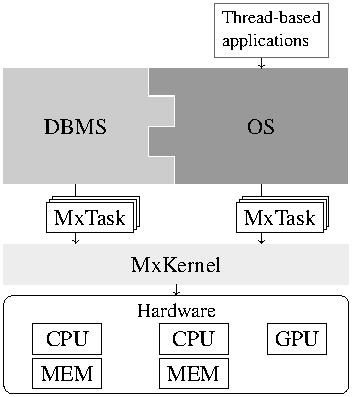
\includegraphics[bb=0 0 169 190]{figure5.pdf}
\caption{%
MxKernel provides a small basis layer for managing shared hardware resources between all applications running on a shared machine, including, e.g., the OS and the DBMS.
}
\label{nollhrm19:plt:mxkernel}
\end{figure}

A first step towards solving these problems in a holistic way is the bare-metal platform MxKernel.
Figure \ref{nollhrm19:plt:mxkernel} depicts an overview of the architecture.
The platform's core is a basis layer, which enables to run all applications as well as the OS side by side.
Note that running an OS is optional.
At the same time, MxKernel provides a detailed view of the hardware and an interface to which an application can communicate its requirements regarding hardware resources or performance expectations.

In particular, it implements services for hardware compatibility and a mechanism for control flow execution.
Moreover, its architecture allows, e.g., the OS and the DBMS to share data structures and algorithms such as B-Trees, which can be used for primary key indexing by the DBMS or for implementing a file system by the OS.

\paragraph*{MxTasks.}

The platform MxKernel introduces \emph{MxTasks} to abstract from and to create an interface to the control flow execution.
MxTasks describe small units of work representing a more lightweight alternative to POSIX Threads.
They are executed atomically by implementing a run-to-completion semantic.
Usually, MxTasks feature only a small sequence of instructions.
As a result, their runtime, memory accesses, and resource requirements are easier to predict and to define than threads.
In addition, MxTasks can be coupled with precise metadata about, e.g., its memory access patterns, its accessed data structures and its preferred NUMA region.
Thus, by annotating \emph{MxTasks} with workload information we employ the same concept of sharing semantics between application, OS, DBMS, and hardware as discussed for \emph{workload classes} in Section~\ref{nollhrm19:sec:hana_wlm} or for \emph{jobs} in Section~\ref{nollhrm19:sec:cpu_cache_partitioning}.

MxKernel creates an execution plan that synchronizes MxTasks for shared-resource accesses and optimizes them for cache and NUMA locality.
Thus, MxKernel functions as a central component for resource management which receives (workload) information in the form of MxTasks with metadata.
Its execution framework then tries to fulfill the requirements of all applications as well as possible.
Applications running on top of an (optional) OS, however, can still choose to use threads instead of MxTasks for compatibility reasons.

Furthermore, MxTasks represent a way to exploit heterogeneous systems by providing different implementations for distinct processing units such as GPUs or CPUs.
Based on system load and the runtime property of a MxTask, MxKernel could then choose the most suitable available hardware for execution.

\paragraph*{Experimental Results.}
As a first use case, we evaluated an index data structure based on the B\textsuperscript{link}-tree~\cite{nollhrm19:Lehman:1981:ELC:319628.319663}.
We implement the insert algorithm described by Lehman and Yao~\cite{nollhrm19:Lehman:1981:ELC:319628.319663}.
However, we modify it to support MxTasks: We spawn a new task for each traversal of a node.
This means that we create a task for looking up the child node to traverse next.
When a task finally finds the matching leaf node, we insert the new value.

While concurrent POSIX Threads accessing the same node of the B\textsuperscript{link}-tree have to be protected using latches, MxTasks benefit from the run-to-completion semantic:
Mapping the traversal of a tree node to a specific processor core ensures that only one task accesses a node at a time.
In addition, we benefit from cache locality because one core accesses the same data structure multiple times.

\begin{figure}
\centering
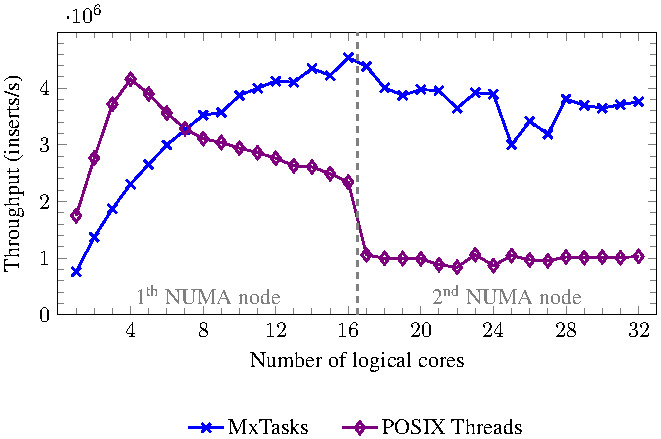
\includegraphics[bb=0 0 317 211]{figure6.pdf}
\caption{Throughput of insert operations into a B\textsuperscript{link}-tree. While the throughput drops down when using more than four POSIX Threads, the throughput stagnates when using MxTasks from the second NUMA region.}
\label{nollhrm19:fig:blinktree:results}
\end{figure}

We consider two different implementations of the B\textsuperscript{link}-tree: a version based on POSIX Threads executed on Linux, and a version based on MxTasks running on MxKernel.
The workload consists of $16 \cdot 10^6$ insert operations using unique key-value pairs.
We execute the experiment on a system with two Intel Xeon E5-2690 processors with 8 CPU cores each, and simultaneous multithreading enabled.

The results illustrated in Figure \ref{nollhrm19:fig:blinktree:results} show that while the thread-based version exhibits a higher throughput until using eight threads, the throughput starts dropping after using four threads.
We explain the differences with the latch contention of the thread version:
Every node has to be protected by a latch to prevent inconsistencies.
MxTasks, on the other hand, have no need to use latches.
Every node of the B\textsuperscript{link}-tree is assigned to one of the cores and every MxTask accessing a node will be executed on the mapped core without suspension.

In addition, we notice that the throughput degrades slightly after using cores from the second NUMA node.
We attribute this to the increased overhead of cache coherency.
For managing MxTasks and tracking their execution state, we use a wait-free queue for every core.
Pushing MxTasks from a queue of one core to the queue of another core, triggers the cache coherency mechanism of the processor which costs additional execution time.
This effect occurs as soon as another NUMA node is involved.
Note that the throughput of the thread-based version, on the other hand, drops significantly with more than 16 cores.


\paragraph*{Conclusion.}
The interaction between DBMS and OS are crucial for creating high-performance systems.
We briefly present how a commercial system such as SAP HANA bypasses the OS and implements, e.g., its own memory management and task scheduling to guarantee robust performance and scaling by exploiting domain-specific knowledge, or to track and to enforce the consumption of hardware resources.
Another strategy is the co-design of DBMS and OS.
As a first step towards this goal, we introduce the bare-metal platform \emph{MxKernel}.
On top of it, the DBMS and the OS run side by side with an interface to communicate their hardware and runtime requirements to.
In return, MxKernel manages hardware resources exclusively.



\section{Conclusion}
\label{nollhrm19:sec:conclusion}

Operational analytics database management systems with the capability to perform both high-speed transactional processing and complex analytical workloads on the same dataset and at the same time, impose new challenges and practical implications for system designers.
In this article, we discussed several solutions that allow to manage these resource-intensive workloads in an efficient and holistic way.
In particular, we explicitly share workload information between application, OS, DBMS, and hardware which allows us to manage resources efficiently and to improve performance and predictability.

By sharing context information between the application and the DBMS, systems can implement an application-aware resource management and quality of service features.
SAP HANA employs \emph{workload classes} for limiting the resource consumption of queries issued by individual applications.
In addition, we presented its \emph{admission control} mechanism to manage the amount of requests the system handles at a given time in order to avoid contention in peak load situations.

By sharing cache usage information between the DBMS and the hardware, we implement a mechanism that \emph{dynamically partitions} the \emph{cache} per individual operator.
We demonstrated that this may improve the overall throughput of highly concurrent workloads, where we restrict the cache usage of scan-intensive operators and increase the cache capacity for cache-sensitive operators.

Finally, we discussed how the database system interacts with the operating system.
While DBMS traditionally take control over individual features of the OS and implement, e.g., a custom memory management or task scheduling, other research directions explore their co-design.
In particular, we presented the bare-metal platform \emph{MxKernel}.
On top of it, the DBMS and the OS run side by side and communicate their hardware and runtime requirements to the platform.
In return, MxKernel takes care of managing all hardware resources.

\section*{Acknowledgments}
This work was supported by DFG, Deutsche Forschungsgemeinschaft, grant number TE 1117/2-1.




\begin{thebibliography}{10}
\itemsep=1pt
\begin{small}
\bibitem{nollhrm19:Plattner:2009:ACA}
H.~Plattner. \newblock A Common Database Approach for OLTP and OLAP Using an In-Memory Column Database. \newblock \emph{SIGMOD}, 2009, pp. 1--2.

\bibitem{nollhrm19:Boehm:2016:OAD}
A.~B{\"{o}}hm, J.~Dittrich, N.~Mukherjee, I.~Pandis, and R.~Sen. \newblock Operational Analytics Data Management Systems. \newblock \emph{VLDB}, vol.~9, no.~13, pp.
1601--1604, 2016.

\bibitem{nollhrm19:Leukert:2015:TIR}
H.~Plattner and B.~Leukert. \newblock The In-Memory Revolution: How SAP HANA Enables Business of the Future. \newblock Springer, 2015.

\bibitem{nollhrm19:Wolf:2014:SUM}
I.~Psaroudakis, F.~Wolf, N.~May, T.~Neumann, A.~B{\"{o}}hm, A.~Ailamaki, and
K.~Sattler. \newblock Scaling up Mixed Workloads: a Battle of Data Freshness, Flexibility, and Scheduling. \newblock \emph{TPCTC}, 2014, pp. 97--112.

\bibitem{nollhrm19:Giceva:2013:COD}
J.~Giceva, T.~Salomie, A.~Sch{\"{u}}pbach, G.~Alonso, and T.~Roscoe. \newblock COD: Database / Operating System Co-Design. \newblock \emph{CIDR}, 2013.

\bibitem{nollhrm19:Giceva:2017:COS}
K.~Kara, J.~Giceva, and G.~Alonso. \newblock FPGA-based Data Partitioning. \newblock \emph{SIGMOD}, 2017, pp. 433--445.

\bibitem{nollhrm19:Boehm:2015:NOT}
A.~B{\"{o}}hm. \newblock Novel Optimization Techniques for Modern Database Environments. \newblock \emph{BTW}, 2015, pp. 23--24.

\bibitem{nollhrm19:Zhang:AWLM:2014}
M.~Zhang. \newblock Autonomic Workload Management for Database Management Systems. \newblock \emph{Ph.D. thesis}, Queen's University, 2014.

\bibitem{nollhrm19:HANA:2018:AdminGuide}
\mbox{SAP SE}.\hspace{1mm}\mbox{SAP HANA Administration Guide}.\hspace{1mm}\url{https://help.sap.com/viewer/6b94445c94ae495c83a19646e7c3fd56/2.0.03/en-US}, 2018.

\bibitem{nollhrm19:Psaroudakis:2015:SUC:2824032.2824043}
I.~Psaroudakis, T.~Scheuer, N.~May, A.~Sellami, and A.~Ailamaki. \newblock Scaling Up Concurrent Main-Memory Column-Store Scans: Towards Adaptive NUMA-aware Data and Task Placement. \newblock \emph{VLDB}, vol.~8, no.~12, pp. 1442--1453,
2015.

\bibitem{nollhrm19:Noll:2018}
S.~Noll, J.~Teubner, N.~May, and A.~B\"{o}hm. \newblock Accelerating Concurrent Workloads with CPU Cache Partitioning. \newblock \emph{ICDE}, 2018,
pp. 437--448.

\bibitem{nollhrm19:Intel:2015:CAT:whitepaper}
Intel Corporation. \newblock Improving Real-Time Performance by Utilizing Cache Allocation Technology. \newblock \emph{White paper}, 2015.

\bibitem{nollhrm19:Lee:2009:MMC:1687627.1687670}
R.~Lee, X.~Ding, F.~Chen, Q.~Lu, and X.~Zhang. \newblock MCC-DB: Minimizing Cache Conflicts in Multi-core Processors for Databases. \newblock \emph{VLDB},
vol.~2, no.~1, pp. 373--384, 2009.

\bibitem{nollhrm19:4658653}
J.~Lin, Q.~Lu, X.~Ding, Z.~Zhang, X.~Zhang, and P.~Sadayappan. \newblock Gaining Insights into Multicore Cache Partitioning: Bridging the Gap Between Simulation and Real Systems. \newblock \emph{HPCA}, IEEE Computer Society, 2008, pp. 367--378.

\bibitem{nollhrm19:Zhang:2009:TPP:1519065.1519076}
X.~Zhang, S.~Dwarkadas, and K.~Shen. \newblock Towards Practical Page Coloring-based Multicore Cache Management. \newblock \emph{EuroSys}, ACM, 2009, pp. 89--102.

\bibitem{nollhrm19:Intel:2017:CAT:Kernel}
Intel Corporation. \newblock User Interface for Resource Allocation in Intel Resource Director Technology. \newblock Documentation of the Linux Kernel, \url{https://www.kernel.org/doc/Documentation/x86/intel_rdt_ui.txt}, 2017.

\bibitem{nollhrm19:Chou:1985:EBM:1286760.1286772}
H.-T. Chou and D.~J. DeWitt. \newblock An Evaluation of Buffer Management Strategies for Relational Database Systems. \newblock \emph{VLDB}, 1985, pp. 127--141.

\bibitem{nollhrm19:Tam:2009:RAL:1508244.1508259}
D.~K. Tam, R.~Azimi, L.~B. Soares, and M.~Stumm. \newblock RapidMRC: Approximating L2 Miss Rate Curves on Commodity Systems for Online Optimizations. \newblock \emph{ASPLOS}, ACM, 2009, pp.
121--132.

\bibitem{nollhrm19:Manegold:2002:GDC:1287369.1287387}
S.~Manegold, P.~Boncz, and M.~L. Kersten. \newblock Generic Database Cost Models for Hierarchical Memory Systems. \newblock \emph{VLDB}, 2002, pp. 191--202.

\bibitem{nollhrm19:Zhou:2004:DTP:1024393.1024415}
P.~Zhou, V.~Pandey, J.~Sundaresan, A.~Raghuraman, Y.~Zhou, and S.~Kumar. \newblock Dynamic Tracking of Page Miss Ratio Curve for Memory Management. \newblock \emph{ASPLOS}, ACM, 2004, pp.
177--188.

\bibitem{nollhrm19:IBM:2004:DB2Memory}
IBM. \newblock The DB2 UDB memory model -- How DB2 uses memory. \newblock \url{https://www.ibm.com/developerworks/data/library/techarticle/dm-0406qi/}, 2018.

\bibitem{nollhrm19:Oracle:2018:Memory}
Oracle. \newblock Database Administrator’s Guide -- Managing Memory. \newblock \url{https://docs.oracle.com/database/121/ADMIN/memory.htm}, 2018.

\bibitem{nollhrm19:Oukid:2017:MMT:3137628.3137629}
I.~Oukid, D.~Booss, A.~Lespinasse, W.~Lehner, T.~Willhalm, and G.~Gomes. \newblock Memory Management Techniques for Large-Scale. Persistent-Main-Memory Systems. \newblock \emph{VLDB}, vol.~10, no.~11, pp. 1166--1177, 2017.

\bibitem{nollhrm19:PsaroudakisSMA13}
I.~Psaroudakis, T.~Scheuer, N.~May, and A.~Ailamaki. \newblock Task Scheduling for Highly Concurrent Analytical and Transactional Main-Memory Workloads. \newblock \emph{ADMS}, 2013, pp. 36--45.

\bibitem{nollhrm19:Psaroudakis:2016:AND:3015274.3015275}
I.~Psaroudakis, T.~Scheuer, N.~May, A.~Sellami, and A.~Ailamaki. \newblock Adaptive NUMA-aware Data Placement and Task Scheduling for Analytical Workloads in Main-Memory Column-Stores. \newblock \emph{VLDB}, vol.~10, no.~2, pp. 37--48, 2016.

\bibitem{nollhrm19:kleen2005numa}
A.~Kleen. \newblock A NUMA API for Linux. \newblock \emph{White paper}, SUSE Labs, 2004.

\bibitem{nollhrm19:Lehman:1981:ELC:319628.319663}
P.~L. Lehman and S.~B. Yao. \newblock Efficient Locking for Concurrent Operations on B-Trees. \newblock \emph{ACM Trans. Database Syst.}, vol.~6, no.~4, pp. 650--670, 1981.
\end{small}
\end{thebibliography}

\end{document}

\end{article}
%
\begin{article}
{Leveraging Hyperupcalls To Bridge The Semantic Gap: An Application Perspective}
{Michael Wei, Nadav Amit}
\graphicspath{{submissions/mwei/figs/}}
\documentclass[11pt]{article}
%\documentclass[11pt,dvipdfm]{article}

\usepackage{deauthor}
\usepackage{url}            % simple URL typesetting
\usepackage{graphicx}
\usepackage{times}
\usepackage{fancyvrb}
\usepackage{comment}

% \graphicspath{{authorname/}}

\begin{document}

%\title{MLflow: An Open Platform for Machine Learning Experimentation, Reproducibility and Production}
%\title{MLflow: An Open Platform for the End-to-End Machine Learning Lifecycle}
\title{Accelerating the Machine Learning Lifecycle with {MLflow}}

% The \author macro works with any number of authors. There are two
% commands used to separate the names and addresses of multiple
% authors: \And and \AND.
%
% Using \And between authors leaves it to LaTeX to determine where to
% break the lines. Using \AND forces a line break at that point. So,
% if LaTeX puts 3 of 4 authors names on the first line, and the last
% on the second line, try using \AND instead of \And before the third
% author name.

\author{
  \textbf{Matei Zaharia, Andrew Chen, Aaron Davidson, Ali Ghodsi, Sue Ann Hong, Andy Konwinski,}\\
  \textbf{Siddharth Murching, Tomas Nykodym, Paul Ogilvie, Mani Parkhe, Fen Xie, Corey Zumar} \\
  Databricks Inc.\\
  %% examples of more authors
  %% \And
  %% Coauthor \\
  %% Affiliation \\
  %% Address \\
  %% \texttt{email} \\
  %% \AND
  %% Coauthor \\
  %% Affiliation \\
  %% Address \\
  %% \texttt{email} \\
  %% \And
  %% Coauthor \\
  %% Affiliation \\
  %% Address \\
  %% \texttt{email} \\
  %% \And
  %% Coauthor \\
  %% Affiliation \\
  %% Address \\
  %% \texttt{email} \\
}

\maketitle

\begin{abstract}
Machine learning development creates multiple new challenges that are not present in a traditional software development lifecycle.
These include keeping track of the myriad inputs to an ML application (e.g., data versions, code and tuning parameters), reproducing results, and production deployment.
In this paper, we summarize these challenges from our experience with Databricks customers, and describe MLflow, an open source platform we recently launched to streamline the machine learning lifecycle.
MLflow covers three key challenges: experimentation, reproducibility, and model deployment, using generic APIs that work with any ML library, algorithm and programming language.
The project has a rapidly growing open source community, with over 50 contributors since its launch in June 2018.
\end{abstract}

\section{Introduction}

Machine learning development requires solving new problems that are not part of the standard software development lifecycle.
For example, while traditional software has a well-defined set of product features to be built, ML development tends to revolve around \emph{experimentation}: the ML developer will constantly experiment with new datasets, models, software libraries, tuning parameters, etc.~to optimize a business metric such as model accuracy.
Because model performance depends heavily on the input data and training process, \emph{reproducibility} is paramount throughout ML development.
Finally, in order to have business impact, ML applications need to be \emph{deployed} to production, which means both deploying a model in a way that can be used for inference (e.g., REST serving) and deploying scheduled jobs to regularly update the model.
This is especially challenging when deployment requires collaboration with another team, such as application engineers who are not ML experts.

Based on our conversations with dozens of Databricks customers that use machine learning, these lifecycle problems are a major bottleneck in practice.
Although today's ML libraries provide tools for part of the lifecycle, there are no standard systems and interfaces to manage the full process.
For example, TensorFlow offers a training API and a Serving system~\cite{tfx}, but TensorFlow Serving cannot easily be used for models from another ML library, or from an incompatible version of TensorFlow.
In practice, an organization will need to run models from multiple ML libraries, TensorFlow versions, etc., and has to design its own infrastructure for this task.


Faced with these challenges, many organizations try to ``lock down'' the ML development process to obtain reproducibility and deployability.
Some organizations develop internal guidelines for ML development, such as which libraries one can use that the production team will support.
Others develop internal \emph{ML platforms} (e.g., Facebook's FBLearner~\cite{fblearner}, Uber's Michelangelo~\cite{michelangelo} and Google's TFX~\cite{tfx}): APIs that ML developers must use in order to build deployable models.
Unfortunately, both approaches limit ML developers in the algorithms and libraries they can use, decreasing their ability to experiment, and both create substantial engineering work whenever the ML developers want to use new libraries or models.

%Some organizations ask each ML team to manage its own infrastructure, which is expensive.
%Others try to develop shared \emph{ML platforms} that data scientists must use to build their models (e.g., Facebook's FBLearner~\cite{fblearner} and Uber's Michelangelo~\cite{michelangelo}), but this approach also has challenges, because model developers are limited to the algorithms and libraries supported by the platform and cannot easily experiment with others.

In this paper, we summarize our experience with ML lifecycle challenges at Databricks customers and describe MLflow, an open source ML platform we are developing to address these challenges.
MLflow's key principle is an \emph{open interface} design, where data scientists and engineers can bring their own training code, metrics, and inference logic while benefitting from a structured development process.
%MLflow leverages simple, generic interfaces such as Docker containers and REST APIs to achieve this goal.
For example, a ``model'' saved in MLflow can simply be a Python function (and associated library dependencies) that MLflow then knows how to deploy in various environments (e.g., batch or real-time scoring).
Other MLflow abstractions are likewise based on generic interfaces, such as REST APIs and Docker containers.
Compared to existing ML platforms like FBLearner, Michelangelo and TFX, this open interface design gives users flexibility and control while retaining the benefits of lifecycle management.
%Moreover, MLflow's open source nature enables easily sharing ML work across organizations.
The current version of MLflow provides APIs for experiment tracking, reproducible runs and model packaging and deployment, usable in Python, Java and R.
We describe these APIs and some sample MLflow use cases to show how the system can streamline the machine learning lifecycle.

\section{Challenges in Machine Learning Development}

ML faces many of the challenges in traditional software development, such as testing, code review, monitoring, etc.
In other ways, however, ML applications are different from traditional software, and present new problems.

One of the main differences is that the goal in machine learning is to \emph{optimize} a specific metric, such as prediction accuracy, instead of simply meeting a set of functional requirements.
For example, for a retailer, every 1\% improvement in prediction accuracy for a recommendation engine might lead to millions of dollars in revenue, so the ML team working on this engine will continuously want to improve the model.
This means that ML developers wish to continuously experiment with the latest models, software libraries, etc.,~to improve target metrics.
Beyond this difference in objective, ML applications are more complex to manage because their performance depends on training data, tuning, and concerns such as overfitting that do not occur in other applications.
%This means that reproducibility of these runtime conditions is important.
Finally, ML applications are often developed by teams or individuals with very different expertise, and hand-off between these individuals can be challenging.
For example, a data scientist might be an expert at ML training, and use her skills to create a model, but she might need to pass the model to a software engineer for deployment within an application.
Any errors in this process (e.g., mismatched software versions or data formats) might lead to incorrect results that are hard for a software engineer without ML knowledge to debug.

Based on these requirements in working with ML, we found four challenges to arise repeatedly at ML users:

\vspace{-0.6em}
\paragraph{1. Multitude of tools.} Hundreds of software tools cover each phase of ML development, from data preparation to model training to deployment. However, unlike traditional software development, where teams select \emph{one} tool for each phase, ML developers usually want to try \emph{every} available tool (e.g., algorithm) to see whether it improves results. For example, a team might try multiple preprocessing libraries (e.g., Pandas and Apache Spark) to featurize data; multiple model types (e.g. trees and deep learning); and even multiple frameworks for the same model type (e.g., TensorFlow and PyTorch) to run various models published online by researchers. %This diversity of tools means that ML teams need to use and productionize dozens of libraries.

\vspace{-0.6em}
\paragraph{2. Experiment tracking.} Machine learning results are affected by dozens of configurable parameters, ranging from the input data to hyperparameters and preprocessing code. Whether an individual is working alone or on a team, it is difficult to track which parameters, code, and data went into each experiment to produce a model.

\vspace{-0.6em}
\paragraph{3. Reproducibility.} Without detailed tracking, teams often have trouble getting the same code to work again. For example, a data scientist passing her training code to an engineer for use in production might see problems if the engineer modifies it, and even a user working alone needs to reliably reproduce old results to stay productive. %Even ML researchers frequently experience this problem when trying to reproduce published work.

\vspace{-0.6em}
\paragraph{4. Production deployment.} Moving an application to production can be challenging, both for inference and training. First, there are a plethora of possible inference environments, such as REST serving, batch scoring and mobile applications, but there is no standard way to move models from any library to these diverse environments. Second, the model training pipeline also needs to be reliably converted to a scheduled job, which requires care to reproduce the software environments, parameters, etc.~used in development.
Production deployment is especially challenging because it often requires passing the ML application to a different team with less ML expertise.

~

\vspace{-0.6em}
To address these problems, we believe that ML development processes should be explicitly designed to promote reproducibility, deployability, etc. The challenge is how to do so while leaving maximum flexibility for ML developers to build the best possible model. This led us to the open interface design philosophy for MLflow.

\section{MLflow Overview}

To structure the ML development process while leaving users maximum flexibility, we built MLflow around an \emph{open interface} philosophy: the system should define general interfaces for each abstraction (e.g., a training step, a deployment tool or a model) that allow users to bring their own code or workflows.
For example, many existing ML tools represent models using a serialization format, such as TensorFlow graphs~\cite{abadi2016tensorflow}, ONNX~\cite{onnx} or PMML~\cite{pmml}, when passing them from training to serving. This restricts applications to using specific libraries.
In contrast, in MLflow, a model can be represented simply as a Python function (and library dependency information), so any development tool that knows how to run a Python function can run such a model.
For more specialized deployment tools, a model can also expose other interfaces called ``flavors" (e.g., an ONNX graph) while still remaining viewable as just a Python function.
As another example, MLflow exposes most of its features through REST APIs that can called from any programming language.

More specifically, MLflow provides three components, which can either be used together or separately:

\begin{itemize}
\item \textbf{MLflow Tracking}, which is an API for recording experiment runs, including code used, parameters, input data, metrics, and arbitrary output files. These runs can then be queried through an API or UI.

\item\textbf{MLflow Projects}, a simple format for packaging code into reusable projects. Each project defines its environment (e.g., software libraries required), the code to run, and parameters that can be used to call the project programmatically in a multi-step workflow or in automated tools such as hyperparameter tuners.

\item\textbf{MLflow Models}, a generic format for packaging models (both the code and data required) that can work with diverse deployment tools (e.g., batch and real-time inference). %The goal is to give users of the model (e.g., a production engineer) a consistent interface for working with models built in different tools.
\end{itemize}

%We next sketch these components in turn; full documentation on them is available at \url{mlflow.org}.

\subsection{MLflow Tracking}

MLflow Tracking is an API for logging and querying \emph{experiment runs}, which consist of parameters, code versions, metrics and arbitrary output files called \emph{artifacts}. Users can start/end runs and log metrics, parameters and artifacts using simple API calls, as shown below using MLflow's Python API:

\begin{Verbatim}[frame=single,fontsize=\small,samepage=true]
# Log parameters, which are arbitrary key-value pairs
mlflow.log_param("num_dimensions", 8)
mlflow.log_param("regularization", 0.1)

# Log metrics; each metric can also be updated throughout the run
mlflow.log_metric("accuracy", 0.8)
mlflow.log_metric("r2", 0.4)

# Log artifacts (arbitrary output files)
mlflow.log_artifact("precision_recall.png")
\end{Verbatim}

MLflow Tracking API calls can be inserted anywhere users run code (e.g., standalone applications or Jupyter notebooks running in the cloud). The tracking API logs results to a local directory by default, but it can also be configured to log over the network to a server, allowing teams to share a centralized MLflow tracking server and compare results from multiple developers.

Once users have recorded runs, MLflow allows users to query them through an API or web-based UI (Figure~\ref{fig:tracking-ui}). This UI includes the ability to organize runs into groups called Experiments, search and sort them, and compare groups of runs, enabling users to build a custom leaderboard for each of their ML problems and even compare results across teams. The UI is inspired by experiment visualization tools such as Sacred~\cite{sacred}, ModelDB~\cite{modeldb} and TensorBoard~\cite{tensorboard}, and supports similar visualizations and queries.

\begin{figure}[h]
\centering
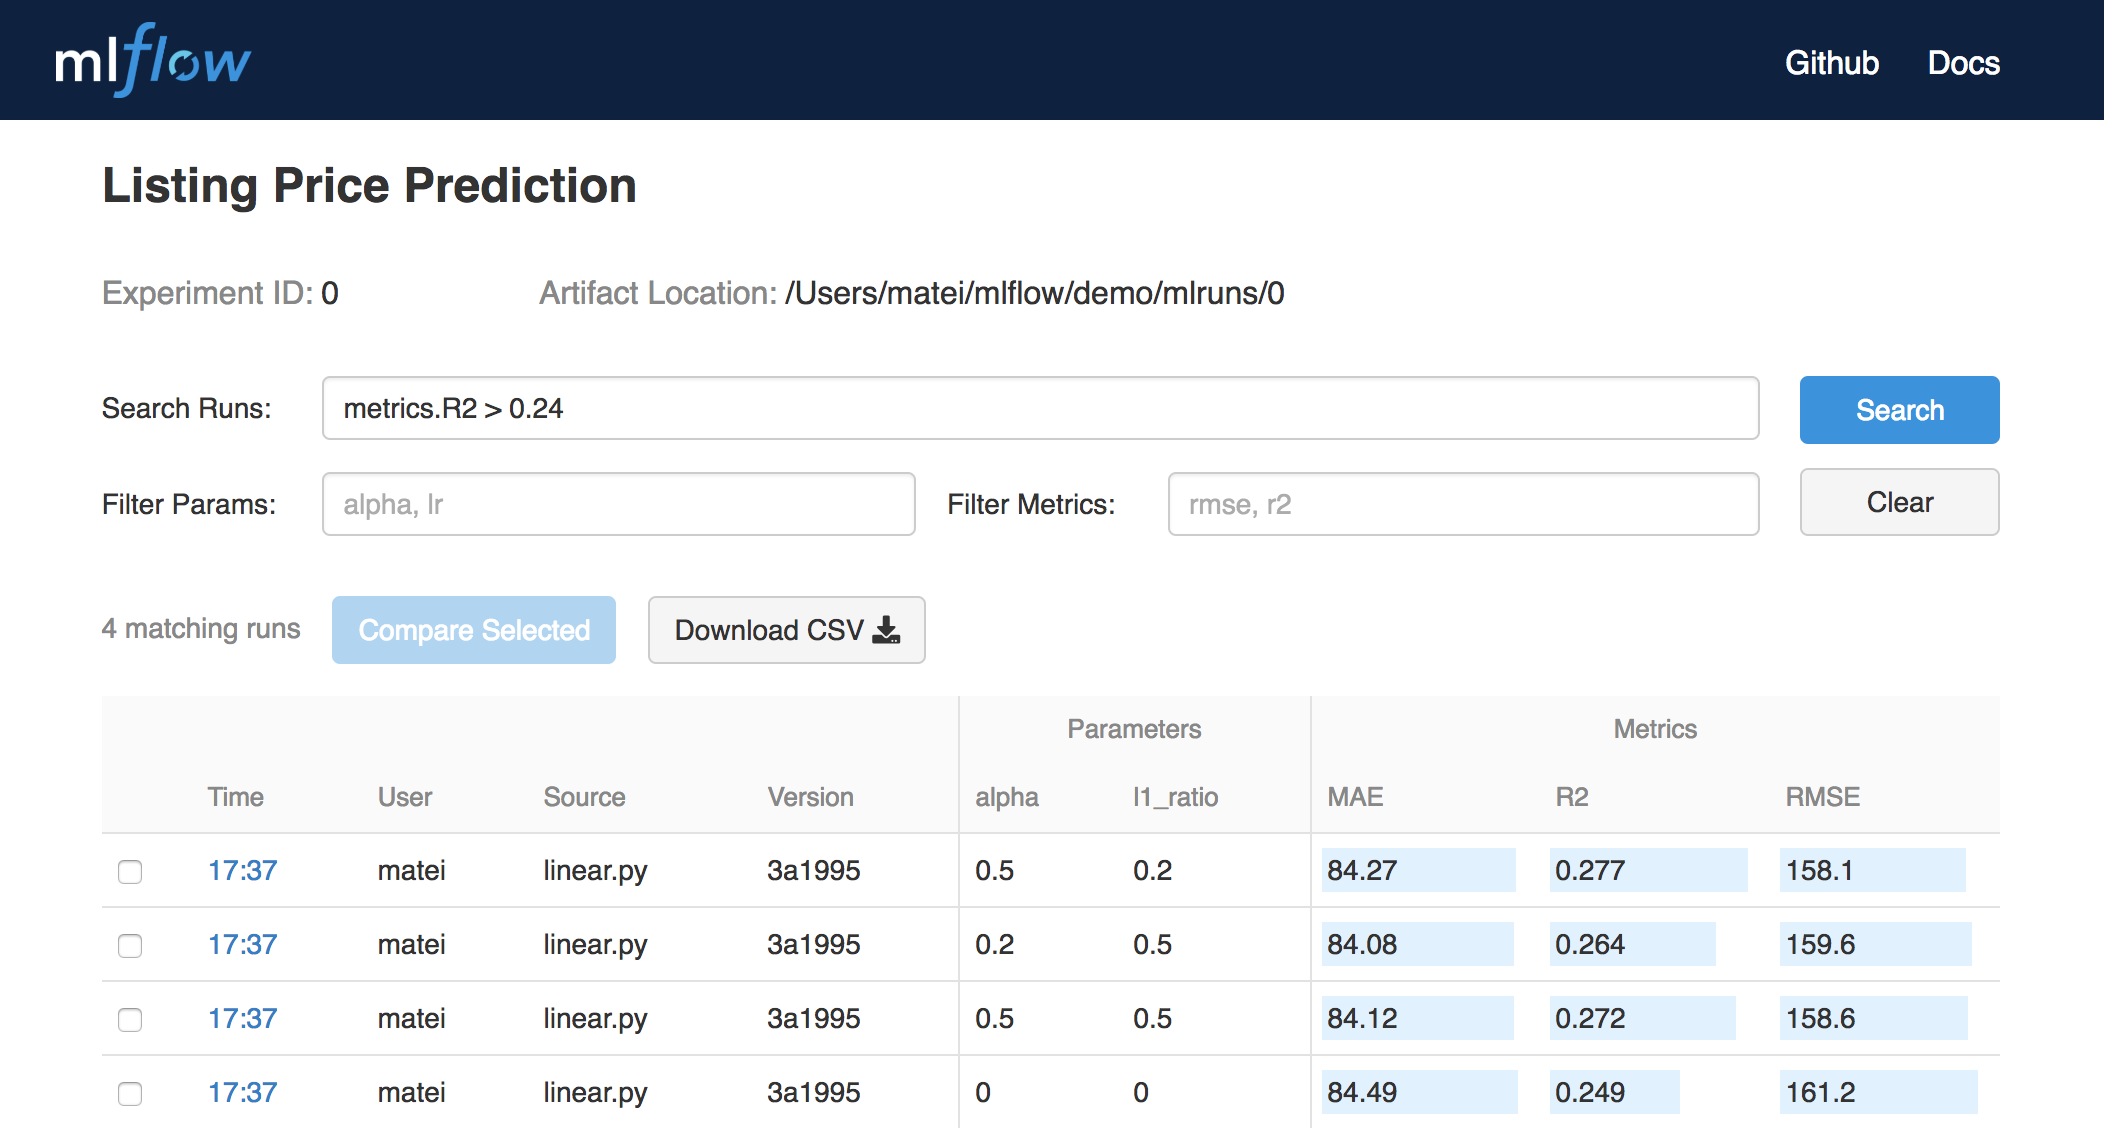
\includegraphics[bb=0 0 1052 564,width=\textwidth]{tracking.png}
\caption{MLflow Tracking UI showing several runs in an experiment. Clicking each run lists its metrics, artifacts and output details and lets the user post comments about the run.}
\label{fig:tracking-ui}
\end{figure}

\subsection{MLflow Projects}

MLflow Projects provide a simple format for packaging reproducible data science code. Each project is simply a directory with code or a Git repository, and uses a descriptor file to specify its dependencies and how to run the code. A MLflow Project is defined by a simple YAML file called MLproject, as shown below:

\begin{Verbatim}[frame=single,fontsize=\small,samepage=true]
name: My Project
conda_env: conda.yaml
entry_points:
  main:
    parameters:
      data_file: path
      alpha: {type: float, default: 0.1}
    command: "python train.py --reg-param {alpha} --data {data_file}"
\end{Verbatim}


Projects can specify their dependencies through a Conda environment or (in an upcoming release) a Docker container specification. A project may also have multiple entry points for invoking runs, with named parameters that downstream users can provide without understanding the internals of the project.

Users can run projects using the \texttt{mlflow run} command line tool, either from local files or a Git repository:

\begin{Verbatim}[frame=single,fontsize=\small,samepage=true]
mlflow run git@github.com:databricks/mlflow-example.git -P alpha=0.5
\end{Verbatim}

Alternatively, projects can be called programmatically using MLflow's API. This can be used to implement multi-step workflows or to pass projects a ``black box'' into automated tools such as hyperparameter search~\cite{hyperopt}.

In either case, MLflow will automatically set up the project's runtime environment and execute it. If the code inside the project uses the MLflow Tracking API, MLflow will also remember the project version executed (that is, the Git commit) and show an \texttt{mlflow run} command to re-execute it in its UI. Finally, MLflow projects can also be submitted to cloud platforms such as Databricks for remote execution.

\subsection{MLflow Models}

MLflow Models are a convention for packaging machine learning models in multiple formats called ``flavors'', allowing diverse tools to understand the model at different levels of abstractions. MLflow also offers a variety of built-in tools to deploy models in its standard favors. For example, the same model can be deployed as a Docker container for REST serving, as an Apache Spark user-defined function (UDF) for batch inference, or into cloud-managed serving platforms like Amazon SageMaker and Azure ML.

Each MLflow Model is simply stored as a directory containing arbitrary files and an MLmodel YAML file that lists the flavors it can be used in and additional metadata about how it was created:

\begin{Verbatim}[frame=single,fontsize=\small,samepage=true]
time_created: 2018-02-21T13:21:34.12
run_id: c4b65fc2c57f4b6d80c6e58a9dcb9f01
flavors:
  sklearn:
    sklearn_version: 0.19.1
    pickled_model: model.pkl
  python_function:
    loader_module: mlflow.sklearn
    pickled_model: model.pkl
\end{Verbatim}

In this example, the model can be used with tools that support either the \texttt{sklearn} or \texttt{python\_function} model flavors. For example, the MLflow SciKit-Learn library knows how to load a \texttt{sklearn} model as a SciKit-Learn Python object, but other deployment tools, such as running the model in a Docker HTTP server, only understand lower-level flavors like \texttt{python\_function}.
In addition, models logged using MLflow Tracking APIs will automatically include a reference to that run's unique ID, letting users discover how they were built.

\section{Example Use Cases}

In this section, we describe three sample MLflow use cases to highlight how users can leverage each component.

\vspace{-0.6em}
\paragraph{Experiment tracking.} A European energy company is using MLflow to track and update hundreds of energy grid models. This team's goal is to build a time series model for every major energy producer (e.g., power plant) and consumer (e.g., factory), monitor these using standard metrics, and combine the predictions to drive business processes such as pricing. Because a single team is responsible for hundreds of models, possibly using different ML libraries, it was important to have a standard development and tracking process. The team has standardized on using Jupyter notebooks for development, MLflow Tracking for metrics, and Databricks jobs for inference.

\vspace{-0.6em}
\paragraph{Reproducible projects.} An online marketplace is using MLflow Projects to package deep learning jobs using Keras and run them in the cloud. Each data scientist develops models locally on his or her laptop using a small dataset, checks them into a Git repository with an MLproject file, and submits remote runs of the project to GPU instances in the cloud for large-scale training or hyperparameter search. Using MLflow Projects makes it easy to create the same software environment in the cloud and share project code between different data scientists.

\vspace{-0.6em}
\paragraph{Model packaging.} The data science team at an e-commerce site is using MLflow Models to package recommendation models for use by application engineers. The technical challenge here was that the recommendation application includes both a standard, ``off-the-shelf'' recommendation model and custom business logic for pre- and post-processing. For example, the application might include custom code to make sure that the recommended items are diverse. This business logic needs to change in sync with the model, and the data science team wants to control both the business logic and the model, without having to submit a patch to the web application each time this logic has to change.
Moreover, the team wants to A/B test distinct models with distinct versions of the processing logic.
The solution was to package both the recommendation model and the custom logic using the \texttt{python\_function} flavor in an MLflow Model, which can then be deployed and tested as a single unit. %This allows production engineers to deploy the recommendation code as they please without the processing logic falling out of sync with the model.

\section{Related Work}

Many software systems aim to simplify ML development.
The closest to our work are the end-to-end ``ML platforms'' at large web companies.
For example, Facebook's FBLearner lets users write reusable workflow steps that run over data in Apache Hive~\cite{fblearner};
Uber's Michelangelo gives users a toolkit of algorithms to choose from that it can automatically train and deploy~\cite{michelangelo}; and Google's TFX provides data preparation and serving tools around TensorFlow~\cite{tfx}.
Anecdotally, these platforms greatly accelerate ML development, showing the benefits of standardizing the ML lifecycle.
However, they generally restrict users to a specific set of algorithms or libraries, so teams are on their own when they step outside these boundaries.
Our goal in MLflow is to let users easily bring their own tools and software in as many steps in the process as possible through our ``open interface'' design.
This includes custom training steps, inference code, and logged parameters and artifacts.

Other systems also tackle specific problems within the ML lifecycle. For example, Sacred~\cite{sacred}, ModelDB~\cite{modeldb} and TensorBoard~\cite{tensorboard} let users track experiments; PMML~\cite{pmml} and ONNX~\cite{onnx} are cross-library model serialization formats; Clipper~\cite{clipper} can deploy arbitrary models as Docker containers; and CDE~\cite{cde}, CodaLab~\cite{codalab}, Binder~\cite{binder} and Repo2Docker~\cite{repo2docker} enable reproducible software runs. MLflow combines these concepts with new ones, such as multi-flavor model packaging, into a unified system design and API.

\section{Conclusion}

For machine learning to have widespread commercial impact, organizations require the same kinds of reliable engineering processes around ML that exist in other engineering disciplines such as software development. In this paper, we have described some of the key challenges that differentiate ML development from traditional software development, such as experimentation, reproducibility, and reliable production deployment. We have also described MLflow, a software platform that can structure the machine learning lifecycle while giving users broad flexibility to use their own ML algorithms, software libraries and development processes.
MLflow is available as open source software at \url{https://www.mlflow.org}.


{\small

\begin{thebibliography}{10}

  \bibitem{abadi2016tensorflow}
  M.~Abadi, P.~Barham, J.~Chen, Z.~Chen, A.~Davis, J.~Dean, M.~Devin,
    S.~Ghemawat, G.~Irving, M.~Isard, et~al.
  \newblock {TensorFlow: A System for Large-Scale Machine Learning}.
  \newblock In {\em OSDI}, volume~16, pages 265--283, 2016.

  \bibitem{tfx}
  D.~Baylor, E.~Breck, H.-T. Cheng, N.~Fiedel, C.~Y. Foo, Z.~Haque, S.~Haykal,
    M.~Ispir, V.~Jain, L.~Koc, C.~Y. Koo, L.~Lew, C.~Mewald, A.~N. Modi,
    N.~Polyzotis, S.~Ramesh, S.~Roy, S.~E. Whang, M.~Wicke, J.~Wilkiewicz,
    X.~Zhang, and M.~Zinkevich.
  \newblock Tfx: A tensorflow-based production-scale machine learning platform.
  \newblock In {\em Proceedings of the 23rd ACM SIGKDD International Conference
    on Knowledge Discovery and Data Mining}, KDD '17, pages 1387--1395, New York,
    NY, USA, 2017. ACM.

  \bibitem{hyperopt}
  J.~Bergstra, B.~Komer, C.~Eliasmith, D.~Yamins, and D.~D. Cox.
  \newblock Hyperopt: a python library for model selection and hyperparameter
    optimization.
  \newblock {\em Computational Science and Discovery}, 8(1):014008, 2015.

  \bibitem{binder}
  {Binder}.
  \newblock \url{https://mybinder.org}, 2018.

  \bibitem{clipper}
  D.~Crankshaw, X.~Wang, G.~Zhou, M.~J. Franklin, J.~E. Gonzalez, and I.~Stoica.
  \newblock Clipper: A low-latency online prediction serving system.
  \newblock In {\em Proceedings of the 14th USENIX Conference on Networked
    Systems Design and Implementation}, NSDI'17, pages 613--627, Berkeley, CA,
    USA, 2017. USENIX Association.

  \bibitem{fblearner}
  J.~Dunn.
  \newblock Introducing {FBLearner Flow}: Facebook’s {AI} backbone.
  \newblock
    \url{https://code.fb.com/core-data/introducing-fblearner-flow-facebook-s-ai-backbone/}.

  \bibitem{repo2docker}
  J.~Forde, T.~Head, C.~Holdgraf, Y.~Panda, G.~Nalvarte, M.~Pacer, F.~Perez,
    B.~Ragan-Kelley, and E.~Sundell.
  \newblock Reproducible research environments with repo2docker.
  \newblock ICML, 07/2018 2018.

  \bibitem{tensorboard}
  Google.
  \newblock Tensorboard: Visualizing learning.
  \newblock \url{https://www.tensorflow.org/guide/summaries_and_tensorboard}.

  \bibitem{pmml}
  A.~Guazzelli, W.-C. Lin, and T.~Jena.
  \newblock {\em PMML in Action: Unleashing the Power of Open Standards for Data
    Mining and Predictive Analytics}.
  \newblock CreateSpace, Paramount, CA, 2nd edition, 2012.

  \bibitem{cde}
  P.~J. Guo.
  \newblock {CDE}: A tool for creating portable experimental software packages.
  \newblock {\em Computing in Science and Engineering}, 14(4):32--35, 2012.

  \bibitem{michelangelo}
  J.~Hermann and M.~D. Balso.
  \newblock Meet {Michelangelo}: Uber’s machine learning platform.
  \newblock \url{https://eng.uber.com/michelangelo/}.

  \bibitem{sacred}
  {K}laus {G}reff, {A}aron {K}lein, {M}artin {C}hovanec, {F}rank {H}utter, and
    {J}\"urgen {S}chmidhuber.
  \newblock {T}he {S}acred {I}nfrastructure for {C}omputational {R}esearch.
  \newblock In {K}aty {H}uff, {D}avid {L}ippa, {D}illon {N}iederhut, and
    M.~{P}acer, editors, {\em {P}roceedings of the 16th {P}ython in {S}cience
    {C}onference}, pages 49 -- 56, 2017.

  \bibitem{codalab}
  P.~Liang et~al.
  \newblock {CodaLab}.
  \newblock \url{https://worksheets.codalab.org}, 2018.

  \bibitem{onnx}
  {ONNX Group}.
  \newblock {ONNX}.
  \newblock \url{https://onnx.ai}.

  \bibitem{modeldb}
  M.~Vartak, H.~Subramanyam, W.-E. Lee, S.~Viswanathan, S.~Husnoo, S.~Madden, and
    M.~Zaharia.
  \newblock Modeldb: A system for machine learning model management.
  \newblock In {\em Proceedings of the Workshop on Human-In-the-Loop Data
    Analytics}, HILDA '16, pages 14:1--14:3, New York, NY, USA, 2016. ACM.

  \end{thebibliography}


}
%\bibliographystyle{abbrv}
%\bibliography{paper}

\end{document}

\end{article}

\begin{article}
{Operating System Support for Data Management on Modern Hardware}
{Jana Giceva}
\graphicspath{{submissions/jgiceva/figs/}}
\pdfminorversion=5
\documentclass[11pt]{article}
\usepackage{deauthor,times,graphicx,caption,microtype}
\usepackage{hyperref}
\usepackage{listings}
\usepackage{booktabs}

\begin{document}

\title{Optimistic Lock Coupling: A Scalable and Efficient General-Purpose Synchronization Method}

\author{Viktor Leis, Michael Haubenschild\raisebox{0.9ex}{$\ast$}, Thomas Neumann\\ Technische Universit{\"a}t M{\"u}nchen \hspace{0.7cm} Tableau Software\raisebox{0.9ex}{$\ast$} \\ {\{leis,neumann\}{@}in.tum.de} \hspace{0.7cm} {mhaubenschild{@}tableau.com\raisebox{0.9ex}{$\ast$}}}

\maketitle

\begin{abstract}
As the number of cores on commodity processors continues to increase, scalability becomes more and more crucial for overall performance.
Scalable and efficient concurrent data structures are particularly important, as these are often the building blocks of parallel algorithms.
Unfortunately, traditional synchronization techniques based on fine-grained locking have been shown to be unscalable on modern multi-core CPUs.
Lock-free data structures, on the other hand, are extremely difficult to design and often incur significant overhead.

In this work, we make the case for Optimistic Lock Coupling as a practical alternative to both traditional locking and the lock-free approach.
We show that Optimistic Lock Coupling is highly scalable and almost as simple to implement as traditional lock coupling.
Another important advantage is that it is easily applicable to most tree-like data structures.
We therefore argue that Optimistic Lock Coupling, rather than a complex and error-prone custom synchronization protocol, should be the default choice for performance-critical data structures.
\end{abstract}

\section{Introduction}

% more and more cores
Today, Intel's commodity server processors have up to 28 cores and its upcoming microarchitecture will have up to 48 cores per socket~\cite{intel}.
Similarly, AMD currently stands at 32 cores and this number is expected to double in the next generation~\cite{amd}.
Since both platforms support simultaneous multithreading (also known as hyperthreading), affordable commodity servers (with up to two sockets) will soon routinely have between 100 and 200 hardware threads.

% data structure scalability is important
With such a high degree of hardware parallelism, efficient data processing crucially depends on how well concurrent data structures scale.
Internally, database systems use a plethora of data structures like table heaps, internal work queues, and, most importantly, index structures.
Any of these can easily become a scalability (and therefore overall performance) bottleneck on many-core CPUs.

% traditional synchronization: fine-grained locks, slow, cache invalidation
Traditionally, database systems synchronize internal data structures using fine-grained reader/writer locks\footnote{In this work, we focus on data structure synchronization rather than high-level transaction semantics and therefore use the term {\em lock} for what would typically be called {\em latch} in the database literature. We thus follow common computer science (rather than database) terminology.}.
Unfortunately, while fine-grained locking makes lock contention unlikely, it still results in bad scalability because lock acquisition and release require writing to shared memory.
Due to the way cache coherency is implemented on modern multi-core CPUs, these writes cause additional cache misses\footnote{The cache coherency protocol ensures that all copies of a cache line on other cores are invalidated before the write can proceed.} and the cache line containing the lock's internal data becomes a point of physical contention.
As a result, any frequently-accessed lock (e.g., the lock of the root node of a B-tree) severely limits scalability.

% lock-free bw-tree: no more latches, but indirections, extremely complex
Lock-free data structures like the Bw-tree~\cite{DBLP:conf/icde/LevandoskiLS13a} (a lock-free B-tree variant) or the Split-Ordered List~\cite{DBLP:journals/jacm/ShalevS06} (a lock-free hash table) do not acquire any locks and therefore generally scale much better than locking-based approaches (in particular for read-mostly workloads).
However, lock-free synchronization has other downsides:
First, it is very difficult and results in extremely complex and error-prone code (when compared to locking).
Second, because the functionality of atomic primitives provided by the hardware (e.g., atomically compare-and-swap 8 bytes) is limited, complex operations require additional indirections within the data structure.
For example, the Bw-tree requires an indirection table and the Split-Ordered List requires ``dummy nodes'', resulting in overhead due to additional cache misses.

% OLC for the win
In this paper we make the case for {\em Optimistic Lock Coupling (OLC)}, a synchronization method that combines some of the best properties of lock-based and lock-free synchronization.
OLC utilizes a special lock type that can be used in two modes:
The first mode is similar to a traditional mutex and excludes other threads by physically acquiring the underlying lock.
In the second mode, reads can proceed optimistically by validating a version counter that is embedded in the lock (similar to optimistic concurrency control).
The first mode is typically used by writers and the second mode by readers.
Besides this special lock type, OLC is based on the observation that optimistic lock validations can be interleaved/coupled---similar to the pair-wise interleaved lock acquisition of traditional lock coupling.
Hence, the name Optimistic Lock Coupling.

OLC has a number of desirable features:
\begin{itemize}
\item By reducing the number of writes to shared memory locations and thereby avoiding cache invalidations, it {\bf scales well} for most workloads.
\item In comparison to unsynchronized code, it requires few additional CPU instructions making it {\bf efficient}.
\item OLC is {\bf widely applicable} to different data structures. It has already been successfully used for synchronizing binary search trees~\cite{DBLP:conf/ppopp/BronsonCCO10}, tries~\cite{artsync}, trie/B-tree hybrids~\cite{DBLP:dblp_conf/eurosys/MaoKM12}, and B-trees~\cite{buzzword}.
\item In comparison to the lock-free paradigm, it is also {\bf easy to use} and requires few modifications to existing, single-threaded data structures.
\end{itemize}
Despite these positive features and its simplicity, OLC is not yet widely known.
The goal of this paper is therefore to popularize this simple idea and to make a case for it.
We argue that OLC deserves to be widely known.
It is a good default synchronization paradigm---more complex, data structure-specific protocols are seldom beneficial.

The rest of the paper is organized as follows.
Section~\ref{sec:related} discusses related work, tracing the history of OLC and its underlying ideas in the literature.
The core of the paper is Section~\ref{sec:olc}, which describes the ideas behind OLC and how it can be used to synchronize complex data structures.
In Section~\ref{sec:evaluation} we experimentally show that OLC has low overhead and scales well when used to synchronize an in-memory B-tree.
We summarize the paper in Section~\ref{sec:conc}.

\newpage
\section{Related Work}\label{sec:related}

Lock coupling has been proposed as a method for allowing concurrent operations on B-trees in 1977~\cite{DBLP:journals/acta/BayerS77}.
This traditional and still widely-used method, described in detail in Graefe's B-tree survey~\cite{DBLP:journals/ftdb/Graefe11}, is also called ``latch coupling'', ``hand-over-hand locking'', and ``crabbing''.
Because at most two locks are held at-a-time during tree traversal, this technique seemingly allows for a high degree of parallelism---in particular if read/write locks are used to enable inner nodes to be locked in shared mode.
However, as we show in Section~\ref{sec:evaluation}, on modern hardware lock acquisition (even in shared mode) results in suboptimal scalability.

An early alternative from 1981 is a B-tree variant called B-link tree~\cite{DBLP:journals/tods/LehmanY81}, which only holds a single lock at a time.
It is based on the observation that between the release of the parent lock and the acquisition of the child lock, the only ``dangerous'' thing that could have happened is the split of a child node (assuming one does not implement merge operations).
Thus, when a split happens, the key being searched might end up on a neighboring node to the right of the current child node.
A B-link tree traversal therefore detects this condition and, if needed, transparently proceeds to the neighboring node.
Releasing the parent lock early is highly beneficial when the child node needs to be fetched from disk.
For in-memory workloads, however, the B-link tree has the same scalability issues as lock coupling (it acquires just as many locks).

The next major advance, Optimistic Latch-Free Index Traversal (OLFIT)~\cite{DBLP:conf/vldb/ChaHKK01}, was proposed in 2001.
OLFIT introduced the idea of a combined lock/update counter, which we call {\em optimistic lock}. % , for lack of a better name,
Based on these per-node optimistic locks and the synchronization protocol of the B-link tree, OLFIT finally achieves good scalability on parallel processors.
The OLFIT protocol is fairly complex, as it requires both the non-trivial B-link protocol and optimistic locks.
Furthermore, like the B-link tree protocol, it does not support merging nodes, and is specific to B-trees (cannot easily be applied to other data structures).

In the following two decades, the growth of main-memory capacity led to much research into other data structures besides the venerable B-tree.
Particularly relevant for our discussion is Bronson et al.'s~\cite{DBLP:conf/ppopp/BronsonCCO10} concurrent binary search tree, which is based on optimistic version validation and has a sophisticated, data structure-specific synchronization protocol.
To the best of our knowledge, this 2010 paper is the first that, as part of its protocol, interleaves version validation across nodes---rather than validating each node separately like OLFIT.
In that paper, this idea is called ``hand-over-hand, optimistic validation'', while we prefer the term Optimistic Lock Coupling to highlight the close resemblance to traditional lock coupling.
Similarly, Mao et al.'s~\cite{DBLP:dblp_conf/eurosys/MaoKM12} Masstree (a concurrent hybrid trie/B-tree) is also based on the same ideas, but again uses them as part of a more complex protocol.

The Adaptive Radix Tree (ART)~\cite{art} is another recent in-memory data structure, which we proposed in 2013.
In contrast to the two data structures just mentioned, it was originally designed with single-threaded performance in mind without supporting concurrency.
To add support for concurrency, we initially started designing a custom protocol called Read-Optimized Write Exclusion (ROWEX)~\cite{artsync}, which turned out to be non-trivial and requires modifications of the underlying data structure\footnote{Note that ROWEX is already easier to apply to existing data structures than the lock-free approach. The difficulty depends on the data structure. Applying ROWEX is hard for B-trees with sorted keys and fairly easy for copy-on-write data structures like the Height Optimized Trie~\cite{hot}---with ART being somewhere in the middle.}.
However, fairly late in the project, we also realized, that OLC {\em alone} (rather than as part of a more complex protocol) is sufficient to synchronize ART.
No other changes to the data structure were necessary.
Both approaches were published and experimentally evaluated in a followup paper~\cite{artsync}, which shows that, despite its simplicity, OLC is efficient, scalable, and generally outperforms ROWEX.

Similar results were recently published regarding B-trees~\cite{buzzword}.
In this experimental study a simple OLC-based synchronization outperformed the Bw-tree~\cite{DBLP:conf/icde/LevandoskiLS13a}, a complex lock-free synchronization approach.
Another recent paper shows that for write-intensive workloads, locking often performs better than lock-free synchronization~\cite{DBLP:conf/cidr/FaleiroA17}.
These experiences indicate that OLC is a general-purpose synchronization paradigm and motivate the current paper.

%foster b-tree\cite{DBLP:journals/tods/GraefeKK12}
%Shasha theory~\cite{DBLP:journals/tods/ShashaG88}

\section{Optimistic Lock Coupling}\label{sec:olc}

% locks suck
The standard technique for inter-thread synchronization is mutual exclusion using fine-grained locks.
In a B-tree, for example, every node usually has its own associated lock, which is acquired before accessing that node.
The problem of locking on modern multi- and many-core processors is that lock acquisition and release require writing to the shared memory location that implements the lock.
This write causes exclusive ownership of the underlying cache line and invalidates copies of it on all other processor cores.
For hierarchical, tree-like data structures, the lock of the root node becomes a point of physical contention---even in read-only workloads and even when read/write locks are used.
Depending on the specific data structure, number of cores, cache coherency protocol implementation, cache topology, whether Non-Uniform Memory Access (NUMA) is used, locking can even result in multi-threaded performance that is worse than single-threaded execution.

% in b-trees this happens very much
The inherent pessimism of locking is particularly unfortunate for B-trees:
Despite the fact that logical modifications of the root node are very infrequent, every B-tree operation must lock the root node during tree traversal\footnote{To a lesser extent this obviously applies to all inner nodes, not just the root.}.
Even the vast majority of update operations (with the exception of splits and merges), only modify a single leaf node.
These observations indicate that a more optimistic approach, which does not require locking inner nodes, would be very beneficial for B-trees.

\subsection{Optimistic Locks}

% optimism to the rescue
As the name indicates, optimistic locks try to solve the scalability issues of traditional locks using an optimistic approach.
Instead of always physically acquiring locks, even for nodes that are unlikely to be modified simultaneously, after-the-fact validation is used to detect conflicts.
This is done by augmenting each lock with a version/update counter that is incremented on every modification.
Using this version counter, readers can optimistically proceed before validating that the version did not change to ensure that the read was safe.
If validation fails, the operation is restarted.

% details on opt locks
Using optimistic locks, a read-only node access (i.e., the majority of all operations in a B-tree) does not acquire the lock and does not increment the version counter.
Instead, it performs the following steps:
\begin{enumerate}
\item read lock version (restart if lock is not free)
\item access node
\item read the version again and validate that it has not changed in the meantime
\end{enumerate}
If the last step (the validation) fails, the operation has to be restarted.
Write operations, on the other hand, are more similar to traditional locking:
\begin{enumerate}
\item acquire lock (wait if necessary)
\item access/write to node
\item increment version and unlock node
\end{enumerate}
Writes can therefore protect a node from other writes.

% similar to locks
As we observed in an earlier paper~\cite{artsync}, because of similar semantics, optimistic locks can be hidden behind an API very similar to traditional read/write locks.
Both approaches have an exclusive lock mode, and acquiring a traditional lock in shared mode is analogous to optimistic version validation.
Furthermore, like with some implementations of traditional read/write locks, optimistic locks allow upgrading a shared lock to an exclusive lock.
Lock upgrades are, for example, used to avoid most B-tree update operations from having to lock inner nodes.
In our experience, the close resemblance of optimistic and traditional locks simplifies the reasoning about optimistic locks;
one can apply similar thinking as in traditional lock-based protocols.

\subsection{Lock Coupling with Optimistic Locks}

\begin{figure}
  \centering
  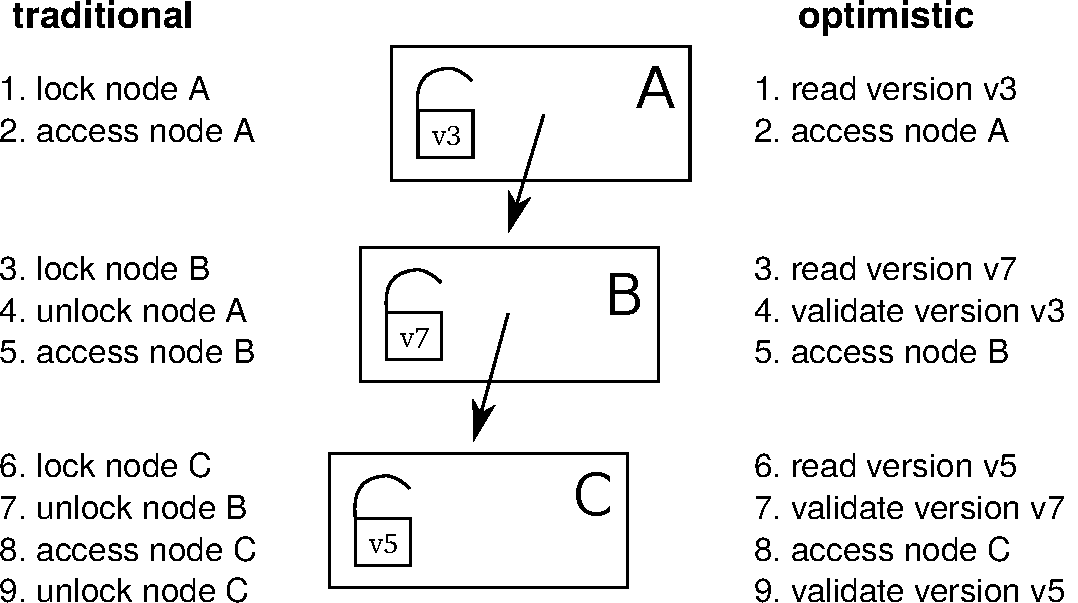
\includegraphics[width=0.65\linewidth]{olcall.pdf}
  \vspace{0.2cm}
  \caption{Comparison of a lookup operation in a 3-level tree using traditional lock coupling (left-hand side) vs.~optimistic lock coupling (right-hand side).}
  \label{fig:olc}
\end{figure}

The traditional and most common lock-based synchronization protocol for B-trees is lock coupling, which interleaves lock acquisitions while holding at most two locks at a time.
If, as we observed earlier, optimistic locks have similar semantics as traditional locks, it is natural to ask whether lock coupling can be combined with optimistic locks.
And indeed the answer is yes: One can almost mechanically translate traditional lock coupling code to optimistic lock coupling code.
This is illustrated in Figure~\ref{fig:olc}, which compares the traversal in a tree of height 3 using traditional and optimistic locks.
As the figure shows, the main difference is that locking is translated to reading the version and that unlocking becomes validation of the previously read version.
This simple change provides efficient lock-free tree traversal without the need to design a complex synchronization protocol.

It is important to emphasize the conceptual simplicity of OLC in comparison to data structures that use custom protocols like the Bw-tree~\cite{DBLP:conf/icde/LevandoskiLS13a}.
To implement lock-free access, the Bw-tree requires an indirection table, delta nodes, complex splitting and merging logic, retry logic, etc.
OLC, on the other hand, can directly be applied to B-trees mostly by adding the appropriate optimistic locking code and without modifying the node layout itself.
Therefore, OpenBw-Tree, an open source implementation of the Bw-tree, requires an order of magnitude more code than a B-tree based on OLC\footnote{Both implementations are available on GitHub: \url{https://github.com/wangziqi2016/index-microbench}}.
Given how difficult it is to develop, validate, and debug lock-free code, simplicity is obviously a major advantage.

\subsection{Correctness Aspects}

\begin{figure}
  % \centering
  %[basicstyle=\normalsize\ttfamily,showstringspaces=false,columns=fullflexible,breaklines=false,breakatwhitespace=true,numbers=none,numberstyle=\small,style=C,keepspaces=true]
\begin{lstlisting}[basicstyle=\ttfamily,language=C++,numbers=left,numberstyle=\small]
std::atomic<BTreeNode*> root;

// search for key in B+tree, returns payload in resultOut
bool lookup(Key key, Value& resultOut) {
   BTreeNode* node = root.load();
   uint64_t nodeVersion = node->readLockOrRestart();
   if (node != root.load()) // make sure the root is still the root
      restart();

   BTreeInner<Key>* parent = nullptr;
   uint64_t parentVersion = 0;

   while (node->isInner()) {
      auto inner = (BTreeInner*)node;

      // unlock parent and make current node the parent
      if (parent)
         parent->readUnlockOrRestart(parentVersion);
      parent = inner;
      parentVersion = nodeVersion;

      // search for next node
      node = inner->findChild(key);
      // validate 'inner' to ensure that 'node' pointer is valid
      inner->checkOrRestart(nodeVersion);
      // now it safe to dereference 'node' pointer (read its version)
      nodeVersion = node->readLockOrRestart();
   }

   // search in leaf and retrieve payload
   auto leaf = (BTreeLeaf*)node;
   bool success = leaf->findValue(key, resultOut);

   // unlock everything
   if (parent)
      parent->readUnlockOrRestart(parentVersion);
   node->readUnlockOrRestart(nodeVersion);

   return success;
}
\end{lstlisting}
  \vspace{0.2cm}
  \caption{B-tree lookup code using OLC. For simplicity, the restart logic is not shown.}
  \label{fig:lookup}
\end{figure}

So far, we have introduced the high-level ideas behind OLC and have stressed its similarity to traditional lock coupling.
Let us now discuss some cases where the close similarity between lock coupling and OLC breaks down.
To make this more concrete, we show the B-tree lookup code in Figure~\ref{fig:lookup}.
In the code, \texttt{readLockOrRestart} reads the lock version and \texttt{readUnlockOrRestart} validates that the read was correct.

One issue with OLC is that any pointer speculatively read from a node may point to invalid memory (if that node is modified concurrently).
Dereferencing such a pointer (e.g., to read its optimistic lock), may cause a segmentation fault or undefined behavior.
In the code shown in Figure~\ref{fig:lookup}, this problem is prevented by the extra check in line 25, which ensures that the read from the node containing the pointer was correct.
Without this additional validation, the code would in line 27 dereference the pointer speculatively read in line 23.
Note that the implementation of \texttt{checkOrRestart} is actually identical to \texttt{readUnlockOrRestart}.
We chose to give it a different name to highlight the fact that this extra check would not be necessary with read/write locks.

Another potential issue with optimistic locks is code that does not terminate.
Code that speculatively accesses a node, like an intra-node binary search, should be written in a way such that it always terminates---even in the presence of concurrent writes.
Otherwise, the validation code that detects the concurrent write will never run.
The binary search of a B-tree, for example, needs to be written in such a way that each comparison makes progress.
For some data structures that do not require loops in the traversal code (like ART) termination is trivially true.

\subsection{Implementation Details}

% implementation, efficiency
To implement an optimistic lock, one can combine the lock and the version counter into a single 64-bit\footnote{Even after subtracting one bit for the lock status, a back-of-the-envelope calculation can show that 63 bits are large enough to never overflow in practice.} word~\cite{artsync}.
A typical read operation will therefore merely consist of reading this version counter atomically.
In C++11 this can be implemented using the \texttt{std::atomic} type.

On x86, atomic reads are cheap because of x86's strong memory order guarantees.
No memory fences are required for sequentially-consistent loads, which are translated (by both GCC and clang) into standard \texttt{MOV} instructions.
Hence, the only effect of \texttt{std::atomic} for loads is preventing instruction re-ordering.
This makes version access and validation cheap.
Acquiring and releasing an optimistic lock in exclusive mode has comparable cost to a traditional lock:
A fairly expensive sequentially-consistent store is needed for acquiring a lock, while a standard \texttt{MOV} suffices for releasing it.
A simple sinlock-based implementation of optimistic locks can be found in the appendix of an earlier paper~\cite{artsync}.

OLC code must be able to handle restarts since validation or lock upgrade can fail due to concurrent writers.
Restarts can easily be implemented by wrapping the data structure operation in a loop (for simplicity not shown in Figure~\ref{fig:lookup}).
Such a loop also enables limiting the number of optimistic retry operations and falling back to pessimistic locking in cases of very heavy contention.
The ability to fall back to traditional locking is a major advantage of OLC in terms of robustness over lock-free approaches, which do not have this option.

In addition to the optimistic shared mode and the exclusive mode, optimistic locks also support a ``shared pessimistic'' mode, which physically acquires the lock in shared mode (allowing multiple concurrent readers but no writers).
This mode is useful for table (or range) scans that touch many tuples on a leaf page (which would otherwise easily abort).
Finally, let us mention that large range scans and table scans, should be broken up into several per-node traversals as is done in the LeanStore~\cite{leanstore} system.

Like all lock-free data structures, but unlike traditional locking and Hardware Transactional Memory~\cite{DBLP:conf/hpca/KarnagelDRLLSL14,DBLP:journals/pvldb/MakreshanskiLS15,htmtkde}, OLC requires care when deleting (and reusing) nodes.
The reason is that a deleting thread can never be sure that a node can be reclaimed because other threads might still be optimistically reading from that node.
Therefore, standard solutions like epoch-based reclamation~\cite{DBLP:conf/sosp/TuZKLM13}, hazard pointers~\cite{DBLP:journals/tpds/Michael04}, or optimized hazard pointers~\cite{DBLP:conf/spaa/BalmauGHZ16} need to be used.
These memory reclamation techniques are, however, largely orthogonal to the synchronization protocol itself.

%-lock-free is not a strong guarantee

\newpage
\section{Evaluation}\label{sec:evaluation}

Let us now experimentally evaluate the overhead and scalability of OLC.
For the experiments, we use an in-memory B+tree implemented in C++11 using templates, which is configured to use nodes of 4096 bytes, random 8 byte keys, and 8 byte payloads.
Based on this B-tree, we compare the following synchronization approaches:
\begin{itemize}
\item an OLC implementation\footnote{An almost identical OLC implementation is available on github: \url{https://github.com/wangziqi2016/index-microbench/tree/master/BTreeOLC}}
\item a variant based on traditional lock coupling and read/write locks
\item the unsynchronized B-tree, which obviously is only correct for read-only workloads but allows measuring the overhead of synchronization
\end{itemize}
Note that earlier work has compared the OLC implementation with a Bw-tree implementation~\cite{buzzword} and other state-of-the-art in-memory index structures.

We use a Haswell EP system with an Intel Xeon E5-2687W v3 CPU, which has 10 cores (20 ``Hyper-Threads'') and 25~MB of L3 cache.
The system is running Ubuntu 18.10 and we use GCC 8.2.0 to compile our code.
The CPU counters are obtained using the Linux perf API\footnote{We use the following convenience wrapper: \url{https://github.com/viktorleis/perfevent}}.

\begin{table}
  \caption{Performance and CPU counters for lookup and insert operations in a B-tree with 100M keys. We perform 100M operations and normalize the CPU counters by that number.}
  \label{tab:overhead}
  \centering
  \begin{tabular}{lrrrrrrr}\toprule
                    &         &        &        & instruc-  & L1     & L3     & branch \\
                    & threads & M op/s & cycles & tions & misses & misses & misses \\\midrule
lookup (no sync.)   & 1       & 1.72   & 2028   & 283     & 39.1   & 14.9   & 16.1   \\
lookup (OLC)        & 1       & 1.65   & 2107   & 370     & 43.9   & 15.1   & 16.7   \\
lookup (lock coup.) & 1       & 1.72   & 2078   & 365     & 42.3   & 16.9   & 15.7   \\\midrule
insert (no sync.)   & 1       & 1.51   & 2286   & 530     & 59.8   & 31.1   & 17.3   \\
insert (OLC)        & 1       & 1.50   & 2303   & 629     & 61.2   & 31.1   & 16.5   \\
insert (lock coup.) & 1       & 1.41   & 2473   & 644     & 61.0   & 31.0   & 17.2   \\\midrule
lookup (no sync.)   & 10      & 15.48  & 2058   & 283     & 38.6   & 15.5   & 16.0   \\
lookup (OLC)        & 10      & 14.60  & 2187   & 370     & 43.8   & 15.8   & 16.8   \\
lookup (lock coup.) & 10      & 5.71   & 5591   & 379     & 54.2   & 17.0   & 14.8   \\\midrule
insert (no sync.)   & 10      & -      & -      & -       & -      & -      & -      \\
insert (OLC)        & 10      & 10.46  & 2940   & 656     & 62.0   & 32.5   & 16.8   \\
insert (lock coup.) & 10      & 7.55   & 4161   & 667     & 75.0   & 28.6   & 16.2   \\
    \bottomrule
\end{tabular}
\end{table}

Table~\ref{tab:overhead} compares the performance and CPU counters for lookup and insert operations in a B-tree with 100M keys.
With {\em single-threaded} execution, we observe that all three approaches have very similar performance.
Adding traditional or optimistic locks to unsynchronized B-tree code results in up to 30\% of additional instructions without affecting single-threaded performance much.

\begin{figure}
  \centering
  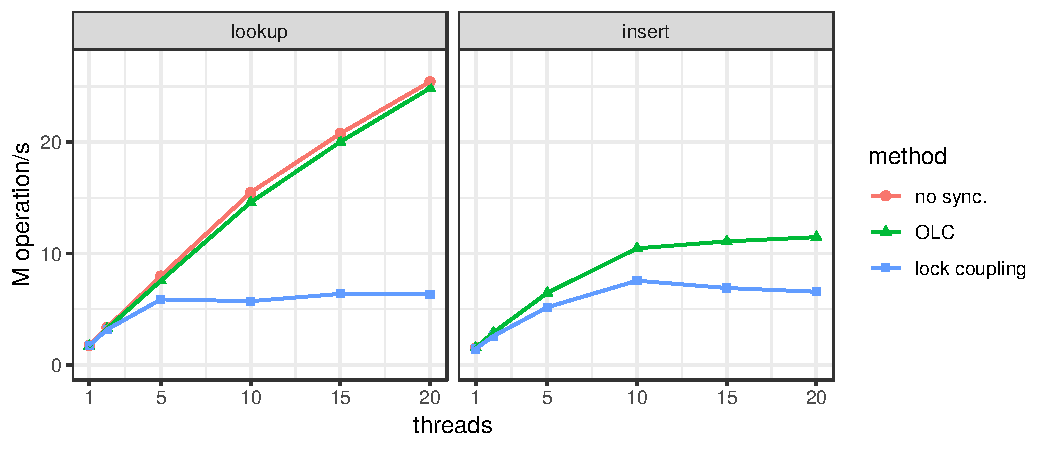
\includegraphics[width=\linewidth]{scale.pdf}
  \vspace{0.2cm}
  \caption{Scalability on 10-core system for B-tree operations (100M values).}
  \label{fig:scale}
\end{figure}

As Figure~\ref{fig:scale} shows, the results change dramatically once we use multiple threads.
For lookup, the scalability of OLC is near-linear up to 20 threads, even though the system has only 10 ``real cores''.
The OLC scalability for insert is also respectable (though not quite as linear because multi-threaded insertion approaches the memory bandwidth of our processor).
The figure also shows that the results of traditional lock coupling with read/write locks are significantly worse than OLC.
With 20 threads, lookup with OLC is 3.9$\times$ faster than traditional lock coupling.

\section{Summary}\label{sec:conc}

Optimistic Lock Coupling (OLC) is an effective synchronization method that combines the simplicity of traditional lock coupling with the superior scalability of lock-free approaches.
OLC is widely applicable and has already been successfully used to synchronize several data structures, including B-trees, binary search trees, and different trie variants.
These features make it highly attractive for modern database systems as well as performance-critical systems software in general.

\begin{thebibliography}{10}

\bibitem{DBLP:conf/spaa/BalmauGHZ16}
O.~Balmau, R.~Guerraoui, M.~Herlihy, and I.~Zablotchi.
\newblock Fast and robust memory reclamation for concurrent data structures.
\newblock In {\em SPAA}, 2016.

\bibitem{DBLP:journals/acta/BayerS77}
R.~Bayer and M.~Schkolnick.
\newblock Concurrency of operations on {B}-trees.
\newblock {\em Acta Informatica}, 9, 1977.

\bibitem{hot}
R.~Binna, E.~Zangerle, M.~Pichl, G.~Specht, and V.~Leis.
\newblock {HOT}: A height optimized trie index for main-memory database
  systems.
\newblock In {\em SIGMOD}, 2018.

\bibitem{DBLP:conf/ppopp/BronsonCCO10}
N.~G. Bronson, J.~Casper, H.~Chafi, and K.~Olukotun.
\newblock A practical concurrent binary search tree.
\newblock In {\em PPOPP}, 2010.

\bibitem{DBLP:conf/vldb/ChaHKK01}
S.~K. Cha, S.~Hwang, K.~Kim, and K.~Kwon.
\newblock Cache-conscious concurrency control of main-memory indexes on
  shared-memory multiprocessor systems.
\newblock In {\em VLDB}, 2001.

\bibitem{intel}
I.~Cutress.
\newblock {Intel} goes for 48-cores: {Cascade-AP} with multi-chip package
  coming soon.
\newblock
  \url{https://www.anandtech.com/show/13535/intel-goes-for-48cores-cascade-ap},
  2018 (accessed January, 2019).

\bibitem{DBLP:conf/cidr/FaleiroA17}
J.~M. Faleiro and D.~J. Abadi.
\newblock Latch-free synchronization in database systems: Silver bullet or
  fool's gold?
\newblock In {\em CIDR}, 2017.

\bibitem{DBLP:journals/ftdb/Graefe11}
G.~Graefe.
\newblock Modern {B}-tree techniques.
\newblock {\em Foundations and Trends in Databases}, 3(4), 2011.

\bibitem{DBLP:conf/hpca/KarnagelDRLLSL14}
T.~Karnagel, R.~Dementiev, R.~Rajwar, K.~Lai, T.~Legler, B.~Schlegel, and
  W.~Lehner.
\newblock Improving in-memory database index performance with
  {Intel}\({}^{\mbox{{\textregistered}}}\) transactional synchronization
  extensions.
\newblock In {\em HPCA}, 2014.

\bibitem{DBLP:journals/tods/LehmanY81}
P.~L. Lehman and S.~B. Yao.
\newblock Efficient locking for concurrent operations on {B}-trees.
\newblock {\em {ACM} Trans. Database Syst.}, 6(4), 1981.

\bibitem{leanstore}
V.~Leis, M.~Haubenschild, A.~Kemper, and T.~Neumann.
\newblock Leanstore: In-memory data management beyond main memory.
\newblock In {\em ICDE}, 2018.

\bibitem{art}
V.~Leis, A.~Kemper, and T.~Neumann.
\newblock The adaptive radix tree: {ARTful} indexing for main-memory databases.
\newblock In {\em ICDE}, 2013.

\bibitem{htmtkde}
V.~Leis, A.~Kemper, and T.~Neumann.
\newblock Scaling {HTM}-supported database transactions to many cores.
\newblock {\em {IEEE} Trans. Knowl. Data Eng.}, 28(2), 2016.

\bibitem{artsync}
V.~Leis, F.~Scheibner, A.~Kemper, and T.~Neumann.
\newblock The {ART} of practical synchronization.
\newblock In {\em DaMoN}, 2016.

\bibitem{DBLP:conf/icde/LevandoskiLS13a}
J.~J. Levandoski, D.~B. Lomet, and S.~Sengupta.
\newblock The {Bw}-tree: A {B}-tree for new hardware platforms.
\newblock In {\em ICDE}, 2013.

\bibitem{DBLP:journals/pvldb/MakreshanskiLS15}
D.~Makreshanski, J.~J. Levandoski, and R.~Stutsman.
\newblock To lock, swap, or elide: On the interplay of hardware transactional
  memory and lock-free indexing.
\newblock {\em {PVLDB}}, 8(11), 2015.

\bibitem{DBLP:dblp_conf/eurosys/MaoKM12}
Y.~Mao, E.~Kohler, and R.~T. Morris.
\newblock Cache craftiness for fast multicore key-value storage.
\newblock In {\em EuroSys}, 2012.

\bibitem{DBLP:journals/tpds/Michael04}
M.~M. Michael.
\newblock Hazard pointers: Safe memory reclamation for lock-free objects.
\newblock {\em {IEEE} Trans. Parallel Distrib. Syst.}, 15(6), 2004.

\bibitem{DBLP:journals/jacm/ShalevS06}
O.~Shalev and N.~Shavit.
\newblock Split-ordered lists: Lock-free extensible hash tables.
\newblock {\em J. {ACM}}, 53(3), 2006.

\bibitem{amd}
A.~Shilov.
\newblock {AMD} previews {EPYC} ‘{Rome}’ processor: Up to 64 {Zen} 2 cores.
\newblock
  \url{https://www.anandtech.com/show/13561/amd-previews-epyc-rome-processor-up-to-64-zen-2-cores},
  2018 (accessed January, 2019).

\bibitem{DBLP:conf/sosp/TuZKLM13}
S.~Tu, W.~Zheng, E.~Kohler, B.~Liskov, and S.~Madden.
\newblock Speedy transactions in multicore in-memory databases.
\newblock In {\em SOSP}, 2013.

\bibitem{buzzword}
Z.~Wang, A.~Pavlo, H.~Lim, V.~Leis, H.~Zhang, M.~Kaminsky, and D.~Andersen.
\newblock Building a {Bw}-tree takes more than just buzz words.
\newblock In {\em SIGMOD}, 2018.

\end{thebibliography}


%\bibliographystyle{abbrv}
%\bibliography{main}

\end{document}

\end{article}

\begin{article}
{The Glass Half Full: Using Programmable Hardware Accelerators in Analytics}
{Zsolt Istv\'{a}n}
\graphicspath{{submissions/zistvan/figs/}}
\documentclass[11pt]{article} 
%\documentclass[11pt,dvipdfm]{article} 

\usepackage{deauthor,times,graphicx} 
%\usepackage[hidelinks]{hyperref}
\usepackage{tcolorbox}

%\graphicspath{{istvan/}} 
\usepackage{xpatch}
\makeatletter

\makeatletter


\begin{document}

\title{The Glass Half Full: Using Programmable \\ Hardware Accelerators in Analytics
}
\author{Zsolt Istv\'{a}n\\ \small IMDEA Software Institute, Madrid, Spain\\  \small \{first.lastname@imdea.org\}}

\maketitle

\begin{abstract}
There have been numeorus proposals to accelerate databases using specialized hardware in past years but 
often the opinion of the community is pessimistic: the performance and energy efficiency benefits of 
specialization are seen to be outweighed by the limitations of the proposed solutions and the 
additional complexity of including specialized hardware, such as field programmable gate arrays (FPGAs), 
in servers. Recently, however, as an effect of stagnating CPU performance, server architectures started to incorporate various programmable hardware components, ranging from smart network interface cards, through SSDs with offloading capabilities, to near-CPU accelerators. The availability of heterogeneous hardware brings opportunities
to databases and we make the case that there is cause for optimism. In the light of a shifting hardware landscape 
and emerging analytics workloads, it is time to revisit our stance on hardware acceleration. 

In this paper we highlight several challenges that have traditionally hindered the deployment of hardware acceleration in databases and explain how they have been alleviated or removed altogether by recent research results and the changing hardware landscape. We also highlight that, now that these challenges have been addressed, a new set of questions emerge around the integration of heterogeneous programmable hardware in tomorrow's databases, for which answers can likely be found only in collaboration with researchers from other fields.

\end{abstract}

\section{Introduction}

There is a rich history of projects aiming to specialize computers (or parts of computers) to databases. Notable examples include the Database Machine from the seventies~\cite{banerjee-databasemachine-79}, Gamma~\cite{dewitt-gamma-1990}, the Netezza data appliance~\cite{francesco-netezza-2011}, the Q100 DB processor~\cite{wu-q100-asplos14}, and Oracle Rapid~\cite{agrawal-rapid-17} most recently. These works demonstrate orders of magnitude increase in energy efficiency and better performance thanks to a hardware/software co-design approach. However, CPUs, until very recently, enjoyed a performance scaling in line with Moore's law and the time and effort of designing and delivering specialized hardware was not economical. This changed with the stagnation in CPU performance~\cite{esmaeilzadeh-darksilicon-isca11} and the simultaneous increase in networking speeds in the last decade that has created a clear need for hardware acceleration. 

Initially, the move to the cloud worked against hardware acceleration for databases due to the cloud's reliance on commodity hardware and the need to cater to many different users and applications. Recently, however, new data-intensive workloads emerged in the cloud (most notably machine learning), that suffered from stagnating CPU performance and could benefit from various types of compute or networking acceleration. If we look at today's cloud offering and datacenters, an exciting, heterogeneous landscape emerges: Machine learning workloads in the Google Cloud are accelerated with Tensor Processing Units (TPUs)~\cite{sato-tpu-google17}, increasing energy efficiency by at least an order of magnitude when compared to GPUs. Amazon, Baidu and Huawei all offer Field Programmable Gate Arrays (FPGAs) by the hour in their cloud to users\footnote{At the moment of writing it costs around \$1.65/h to rent an Amazon EC2 F1 instance.} to implement custom accelerators. Microsoft, in project Catapult~\cite{firestone-catapult-nsdi18}, has been deploying FPGAs in the Azure Cloud to accelerate their infrastructure and machine learning pipelines. Furthermore, Intel has been experimenting with including small programmable elements on their Xeon CPUs~\cite{gupta-harp-fpl16} that can be tailored to accelerate different user applications. 

These recent developments mean that multi-purpose programmable hardware accelerators are entering the mainstream and, from the point of view of the database, they can be exploited without having to incur additional deployment costs. Specialized hardware is most often used to accelerate compute-bound operations and the ongoing shift in the analytical database workloads towards machine learning~\cite{mahajan-danafpga-vldb18}\cite{hellerstein-madlib-vldb12}\footnote{For instance, Microsoft SQL Server now includes machine learning plug-ins. \url{https://docs.microsoft.com/en-us/sql/advanced-analytics/what-is-sql-server-machine-learning}} brings significantly more compute-intensive operations than the core SQL operators. What's more, there are proposals for using machine learning methods to replace parts of the decision making and optimization processes inside databases~\cite{kraska-sage-cidr19}. These emerging operators bring new opportunities in hardware acceleration both inside databases and for user workloads. Furthermore, now that hardware acceleration of real-world workloads is economically feasible, new challenges emerge around deep integration of programmable hardware in databases. 


In this paper we make the case that there is cause for optimism, thanks to the two trends mentioned above, namely, datacenters becoming increasingly heterogeneous and workloads opening towards machine learning. These, combined with the state of the art in hardware acceleration for databases, tackle most of the past hindrances of programmable hardware adoption. We will focus on FPGAs as a representative example and discuss how several significant challenges have been alleviated recently. In the final part of this paper we highlight open questions around the topics of resource management and query planning/compilation in the presence of programmable hardware accelerators.


\section{Background}


\subsection{Programmable Hardware in the Datacenter}


The wide range of programmable hardware devices proposed and already deployed in datacenters can be categorized depending on their location with regards to the data source and CPU into three categories (see Figure~\ref{fig:acceleratorlocations}): on-the-side, in data-path and co-processor.

\begin{figure}[h]
\centering
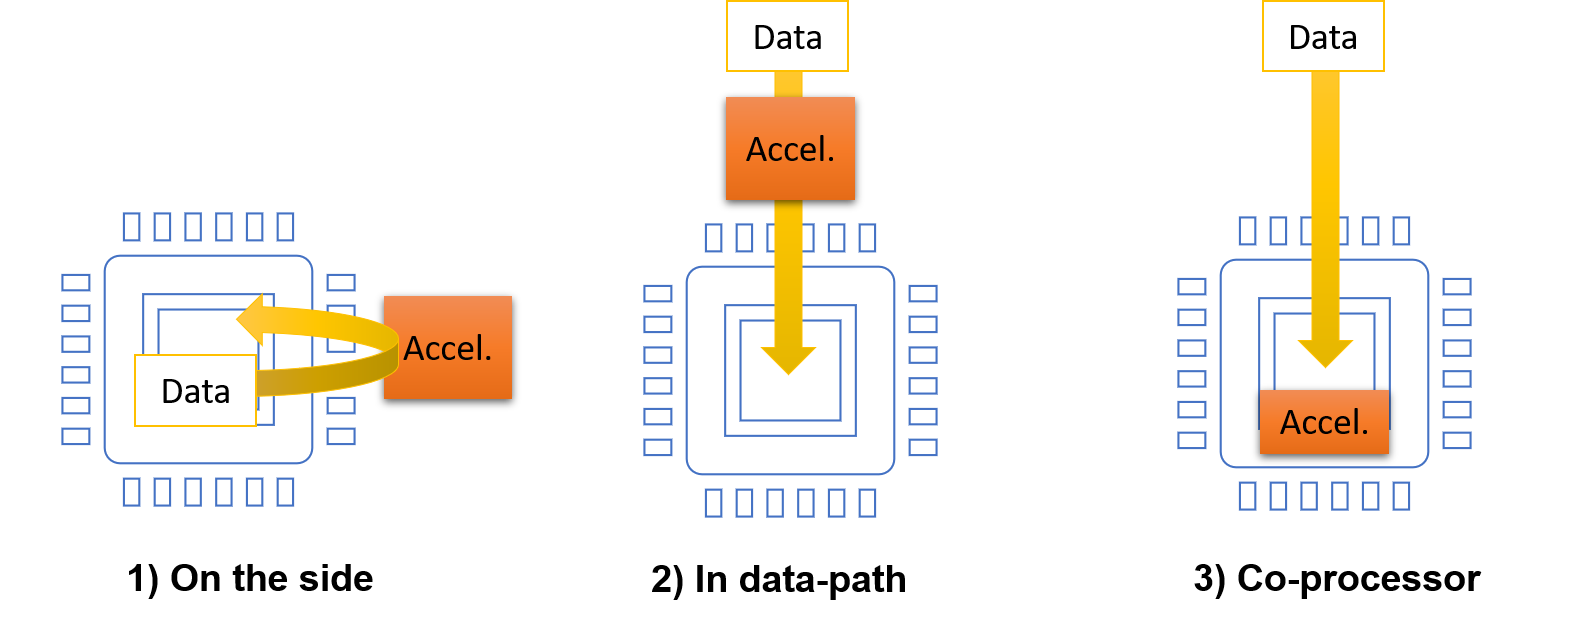
\includegraphics[width=0.75\linewidth]{accelerator-location.png}
\caption{Programmable hardware accelerators can be deployed either as ``on-the-side'' accelerator (e.g., GPUs), as ``in data-path'' accelerator (e.g. smart NICs, smart SSD), or as co-processor (e.g. in Oracle DAX or Intel Xeon+FPGA). \label{fig:acceleratorlocations}}
\end{figure}

The most traditional way we think about accelerators is as being \emph{on-the-side} (Figure~\ref{fig:acceleratorlocations}.1), attached to the processor via an interconnect, for instance PCIe. Importantly, in this deployment scenario the CPU owns the data and explicitly sends it to the accelerator, resulting usually in significant additional latency per operation due to communication latency and data transformation overhead. This encourages offloading operations at large granularity and without requiring back and forth communication between the CPU and the accelerator. GPUs are a common example of this kind of accelerator and were shown to be useful, for instance, to offload LIKE-based string queries~\cite{sitaridi-gpuregex-2016}. There have also been proposals that deploy FPGAs this way for data filtering and decompression, e.g., in the work by Sukhwani et al.~\cite{sukhwani-dbanalyitcs-ieee14}.

Another way of placing acceleration functionality in the architecture is \emph{in data-path} (Figure~\ref{fig:acceleratorlocations}.2). This can be thought of as a generalized version of near-data processing~\cite{oskin-active-ieee98}, and the goal of the accelerator is to filter or transform data at the speed that it is received from the data source. Designs that can't guarantee this could end up slowing down the entire system~\cite{koo-summarizer-micro17}. Much of the research effort in this space has been centered around in-SSD processing~\cite{jo-yoursql-vldb16}\cite{woods-Ibex-vldb14}, but more recently there have been efforts in using RDMA network interface cards (NICs) to accelerate distributed databases~\cite{barthels-join-sigmod15}\cite{dragojevic-farm-debull17}. These NICs are limited to data manipulation acceleration, but there are efforts to make NICs and networking hardware in general more programmable~\cite{bosshart-p4-comrew14}. This will allow offloading in the future complex, application-specific, operations.

The third deployment option, namely, \emph{co-processor} (Figure~\ref{fig:acceleratorlocations}.3), is also becoming increasingly available in the form of CPUs that integrate domain-specific or general-purpose programmable co-processors: The Oracle DAX~\cite{aingaran-dax-hcs16} is an example of the former because it implements database-specific operations, such as data decompression, scan acceleration, comparison-based filtering, on data in the last level cache. Thanks to its specialized nature, it occupies negligible chip space and does not increase the cost of the CPU. As opposed to the DAX, the Intel Xeon+FPGA~\cite{gupta-harp-fpl16} platform offers an FPGA beside the CPU cores for general-purpose acceleration. The FPGA has high bandwidth cache-coherent access to the main memory and can be reprogrammed in different ways. This creates acceleration opportunities without the usual overhead of the on-the-side accelerators.


\subsection{Field Programmable Gate Arrays}

FPGAs are chips that can be programmed to implement arbitrary circuits and historically have been used to prototype and validate designs that would result later in Application-Specific Integrated Circuits (ASICs). They have recently become a target for implementing data processing accelerators in datacenters thanks to their flexibility (their role can change over time, as opposed to an ASIC) and orders of magnitude better energy efficiency than that of traditional CPUs~\cite{teubner-fpgabook-2011}. FPGAs are composed of look-up tables (LUTs), on-chip memory (BRAM) and digital signal processing units (DSPs). All these components can be configured and interconnected flexibly, allowing the programmer to implement custom processing elements (Figure~\ref{fig:insidefpga}). It is not uncommon to have small ARM cores integrated inside the programmable fabric either, e.g., in Xilinx's Zynq product line. 


\begin{figure}[h]
\centering
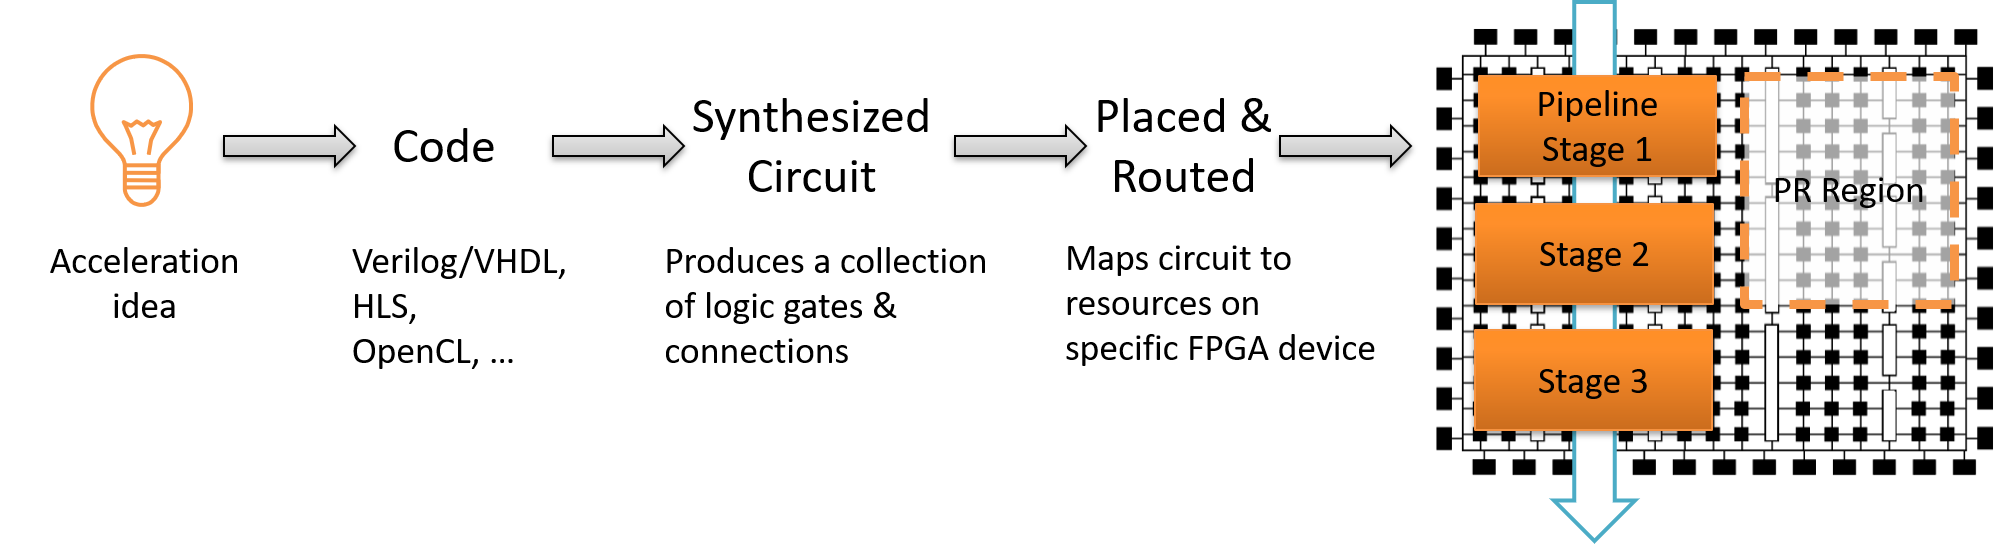
\includegraphics[width=0.9\linewidth]{fpga-internal.PNG}
\vspace{-1em}
\caption{The typical steps of programming FPGAs are shown above. The tools spend most of their time mapping the synthesized circuit onto the FPGA. This is because the chip is composed of many programmable gates and memories that have to be configured and connected together in a 2D space, ensuring that signals can propagate correctly within clock periods.\label{fig:insidefpga}}
\end{figure}


FPGAs offer two types of parallelism: first, pipeline parallelism means that complex functionality can be executed in steps without reducing throughput. The benefit of FPGAs in this context is that the communication between pipeline stages is very efficient thanks to the physical proximity and availability of on-chip memory to construct FIFO buffers. The second type of parallelism that is often exploited on FPGAs is data-parallel execution. This is like SIMD (single instruction multiple data) processing in CPUs, but it can also implement a SPMD (single program multiple data) paradigm if the operations are coarser grained. What makes FPGAs interesting for acceleration is that these two types of parallelism can be combined even inside a single application module to provide both complex processing and scalable throughput.

As Figure~\ref{fig:insidefpga} shows, FPGAs are programmed by synthesizing a circuit from a hardware definition language, such as Verilog or VHLD, and creating a ``bitstream'' for a specific device type that defines the behavior of every logic resource on the chip. This is an expensive step as it requires the tool to lay out the circuit on the ``chip surface'' and define connections and routing of these connections between circuit elements. Since FPGAs have flexible clocking options and the programmer is free to define a target frequency (e.g., 300MHz), the tools have to set up routing such that signals are propagated within the clock periods (which can become impossible with too high frequencies). 

It is also possible to perform partial reconfiguration (PR), meaning that only a portion of the FPGA's resources are reprogrammed (illustrated on the right-hand side of Figure~\ref{fig:insidefpga}). This means that, for instance, in a database use-case a hardware-accelerated operator can be replaced with another one without having to bring the device offline. PR, however, comes with limitations: the regions can only be defined at coarse granularity, their size can't be redefined at runtime and their reprogramming requires milliseconds. 

One important limitation of FPGAs is that all application logic occupies chip space and there is no possibility of ``paging'' code in or out dynamically. This means that the complexity of the operator that is being offloaded is limited by the available logic resources (area) on the FPGA. This also applies to the ``state'' of an algorithm that is often stored as data in the on-chip BRAM memories. These can be accessed in a single clock cycle, but if the data doesn't fit in the available BRAM, high latency off-chip DRAM has to be used. 

\section{Sources of Pessimism}

Many early projects of FPGA-based database acceleration propose deploying them as on-the-side accelerators for row stores~\cite{sukhwani-dbanalyitcs-ieee14}\cite{casper-fpgaacceldb-fccm14}\cite{dennl-sqlaccel-fccm13} and they demonstrate that FPGAs are able to successfully accelerate selection, projection, group-by aggregation, joins and even sorting, by an order of magnitude when compared to MySQL and Postgres, for instance. However, the \textbf{benefits are significantly reduced once one factors in the cost of communication over PCIe and the software overhead} of preparing the data for the FPGA to work on (sometimes pre-parsing, often copying pages). 

In traditional, on-the-side deployments, the high latency communication (microseconds over PCIe) often forces designs to move entire operators onto the FPGA, even if only parts of the operator were a good match for the hardware. This leads to complications, because even though FPGAs excel at parallel and pipelined execution, they behave poorly when an algorithm requires iterative code or has widely branching ``if-then-else'' logic. In the case of the former, CPUs deliver higher performance thanks to their higher clock rates. In the case of the latter, the branching logic needs to be mapped to logic gates that encode all outcomes, resulting in very large circuits. Since the space on the FPGA is limited, the larger circuits result in reduced parallelism, which in turn leads to lower throughput. This means that even though FPGAs could be successful in accelerating the common case of an algorithm, they might not be able to handle corner cases, and in practice this \textbf{leads to uncertainty in the query optimizer or even to wasted work, if an unexpected corner case is encountered during execution}. 

In parallel with accelerator-based efforts, there have been numerous advances in the space of analytical databases. Today, column-oriented databases, such as MonetDB~\cite{boncz-x100-cidr05}, are widely deployed and typically outperform row-oriented ones by at least an order of magnitude and can take advantage of many-core CPUs efficiently. As a result, the \textbf{speedups that FPGAs offer when targeting core SQL operators have shrunk}\footnote{Using specialized hardware can still compete with multi-cores if we factor in energy efficiency (Operations/s/Watt) but in many cases the metric that is of interest is database throughput and response time.} and often are not enough to motivate the additional effort of integrating specialized hardware in the server architecture.

For the above reasons, FPGA-based acceleration ideas are often received with pessimism. However, changes in the hardware available in datacenters and the cloud, as well as the changes in database architecture and user workloads, create novel opportunities for FPGA-based acceleration. In the next section we discuss these in more detail and provide examples of how they can be exploited.







\section{Reasons for Optimism}



\subsection{Changing Architectures}
%Solved challenge 1: data movement overhead -- near-cpu accelerators, capable smartNICs 

With the increasing adoption of distributed architectures for analytical databases, as well as the disaggregation efforts in the datacenter~\cite{klimovic-flash-eurosys16}, there are numerous opportunities for moving computation closer to the data source to reduce the data movement bottlenecks. These bottlenecks arise from the fact that the access bandwidths are higher closer to the data source than over the network/interconnect and they can be eliminated by pushing filtering or similar data reduction operations closer to source. Thus, \textbf{the main goal of accelerators in the data-path is to reduce the amount of data sent to the processor, while maintaining high data access bandwidths.} 


The data source is often (network-attached) flash storage and recent projects, for instance, YourSQL~\cite{jo-yoursql-vldb16}, BlueDBM~\cite{jun-bluedbm-tocs16} and Ibex~\cite{woods-Ibex-vldb14}, show that it is possible to execute SQL operations as the data is moving from storage to processing at high bandwidth. Another use-case that can benefit from data reduction in a similar way is ETL. Recent work~\cite{fang-udp-micro17} has demonstrated that specialized hardware can be used to offer a wide range of ETL operations at high data rate, including: (de)compression, parsing from formats such as CSV or JSON, pattern matching and histogram creation.

In Ibex we deployed an FPGA between an SSD and the CPU, offering several operators that can be plugged into MySQL's query plans. As Figure~\ref{fig:Ibex} shows, these include scans, projection, filtering and group-by aggregation, and were chosen in a way that ensures that processing in hardware will reduce the final data size for most queries. For this reason, Ibex does not accelerate joins, since these would potentially result in larger output than input and slow down the system this way. The rest of the operations are all performed at the rate of the data arriving from storage.


\begin{figure}[h]
\centering
\includegraphics[width=0.7\linewidth]{Ibex.PNG}
\vspace{-1em}
\caption{In Ibex we showcase several operations that can be performed on the data as it is read from storage with the goal of reducing the number of tuples that arrive at the CPU.\label{fig:Ibex}}
\end{figure}

As opposed to on-the-side accelerators, in this space there are two possible options for who ``owns'' the data. In the case of smart SSDs, data is typically managed by the host database~\cite{jo-yoursql-vldb16}\cite{woods-Ibex-vldb14}. In contrast, in the case of distributed storage accessed over the network, it is possible to explore designs where the data is both processed and managed by the specialized hardware device as, for instance, in Caribou~\cite{istvan-caribou-vldb17}\cite{zistvan-diss-2018}, our distributed key-value store that is built using only FPGAs. 

In Caribou, the FPGAs implement, in addition to network line-rate data processing, a hash table data structure and memory allocator necessary for managing large amounts of data, as well as, data replication techniques to ensure that no records are lost or corrupted in case of device failures or network partitions. This results in a high throughput, energy efficient distributed storage layer that, even though is built using FPGAs, can be used as a drop-in replacement for software-based solutions~\cite{zistvan-diss-2018}.



In many ways, in-data-path accelerators provide similar acceleration options as the on-the-side ones because data is still moved over a network (similarly to an interconnect in the case of the latter) that requires processing it in large enough batches to warrant the latency overhead. However, if FPGAs are deployed as co-processors, this overhead is drastically reduced and new opportunities open up, since the latency to the FPGA is in the same order of magnitude as a cross-socket memory access. The Centaur platform~\cite{owaida-centaur-fccm17}, for instance, exposes the FPGA of an Intel Xeon+FPGA platform using an efficient ``hardware thread'' API. As a result, in this co-processor scenario, \textbf{the database can offload functionality as if spawning a parallel thread and the FPGA can be used for processing even just a handful of tuples} -- as we point out in the next subsection, there are emerging use-cases where this low latency acceleration is a game-changer. 

\subsection{Emerging Compute-Intensive Workloads}

%Solved challenge 3: thin margins on core SQL operations -- shift to ML type workloads, DBs becoming more complex themselves, as a sideeffect of CH1 we can now target sub-operator acceleration as well.

The examples in the previous subsection showed how to reduce the data access bottleneck with an in data-path accelerator targeting common SQL operators. It is unclear, however, if this strategy can be applied for co-processors as well.
Modern database engines, that make use of the multi-core CPUs and their wide SIMD units, are rarely compute bound once the data is loaded into main memory. Unless reading data from storage, \textbf{offloading core SQL operators is unlikely to bring orders of magnitudes improvements in performance. There is, however, cause for optimism if we look beyond such operators and in the direction of machine learning}, both training and inference.

A significant portion of machine learning pipelines operate on relational data and the case has been made that there is a benefit in integrating these pipelines directly in the database~\cite{mahajan-danafpga-vldb18}. Furthermore, there is also interest in including such components in the internal modules of the databases~\cite{kraska-sage-cidr19}, to perform optimizations depending on the workload characteristics and the model. Since this could require on-line retraining that, without hardware acceleration, could hurt user throughput significantly, new opportunities open up for FPGAs. Acceleration of training as part of user workloads is being explored, for instance in Dana~\cite{mahajan-danafpga-vldb18}. The iterative and computation-heavy nature of training operators makes them less sensitive to the latency issues introduced by using on-the-side accelerators and therefore could revive the interest in these acceleration platforms. Amazon, for instance, is already offering FPGAs running Xilinx's OpenCL-based compute framework as PCIe-attached accelerators. 

In the ``ML-backed'' database scenario it will also be paramount to be able to take decisions with low latency using learned models -- this further motivates the use of FPGAs. Even though GPUs are a de-facto standard for machine learning acceleration, when it comes to low latency inference, FPGAs can offer benefits since they do not require batching in their processing modules: recent work by Owaida et al.~\cite{owaida-trees-fpl17} and Umuroglu et al.~\cite{umuroglu-finn-fpga17} demonstrates, for instance, how FPGAs can be used very efficiently to accelerate inference using decision trees, respectively, neural networks. 

\subsection{Hybrid Approaches to Acceleration}
\label{sec:hybrid-comp}

Since all functionality, regardless whether used or not, occupies chip space on the FPGA, \textbf{corner cases often can't be efficiently handled in hardware. For this reason, it is important to design accelerators such that they behave predictably even if the particular instance of the problem can't be fully handled.} As we illustrate below with two examples from our work, state of the art solutions overcame such cases by splitting functionality between FPGA and software, such that the part on the FPGA remains beneficial to execution time regardless of the input data contents or distribution. 


\begin{figure}[b]
\centering
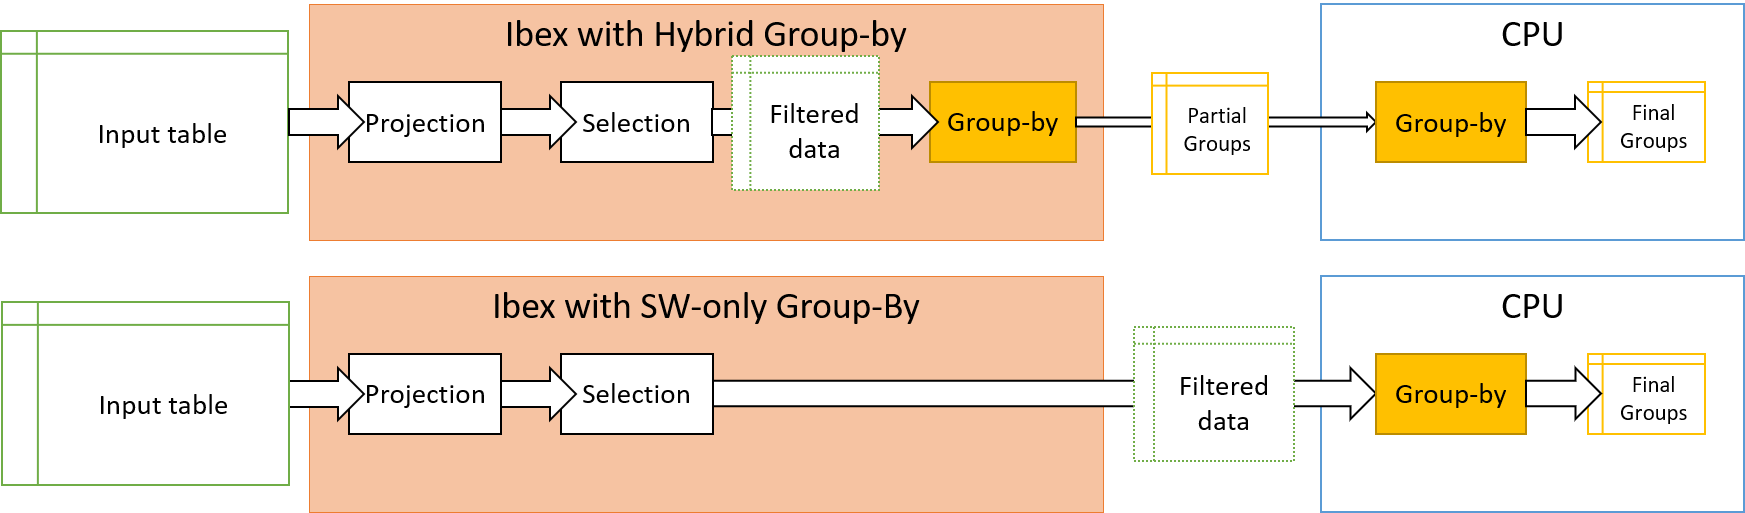
\includegraphics[width=0.9\linewidth]{hybrid-compute.png}
\caption{By implementing operators in a way that allows hybrid computation, the FPGA accelerator can reduce data sizes over the bottleneck connection to the CPU in most cases. In this example of Ibex's group-by operator, if we would choose an ``all or nothing approach'', moving the data to be aggregated to the CPU could become the bottleneck.\label{fig:hybrid-compute}}
\end{figure}


In Ibex~\cite{woods-Ibex-vldb14} we used a hybrid methodology to implement a group-by operator that supports \texttt{min}, \texttt{max}, \texttt{count} and \texttt{sum} (in order to compute \texttt{avg}, we used query rewriting to compute the count and sums). This operator is built around a small hash table that collects the aggregate values. In line with FPGA best-practices, the hash table is of fixed size and is implemented in BRAM. The reason for this is that this way it is possible to guarantee fixed bandwidth operation, regardless of the data contents, because the FPGA doesn't have to pause processing to resize the table. 

Unfortunately, this approach has a drawback: if a query has just one more group than the size of the hash table, the FPGA can't be used -- and this information is often not available up front. We overcome this situation by post-processing the results of the group-by operator on the FPGA in software. The hardware returns results from the group by aggregation unit in a format that allows the database to perform an additional aggregation step without having to apply projections on the tuples or parse them in the first place (see Figure~\ref{fig:hybrid-compute}). If during the hash table operations collisions are encountered that can't be solved, a partial aggregate is evicted from the table and sent to the software post-processor. Once all the data has been processed on the FPGA, the contents of the hash table are sent to the software post-processor to compute the final groups. This results in a behavior where, if all the groups could be computed on the FPGA, the final software step has to perform virtually no work (assuming that the number of resulting groups is significantly smaller than the cardinality of the table), and otherwise the software executes the group by aggregation as if there wasn't any FPGA present (though still benefits from projections and selections).



\begin{figure}[t]
\centering
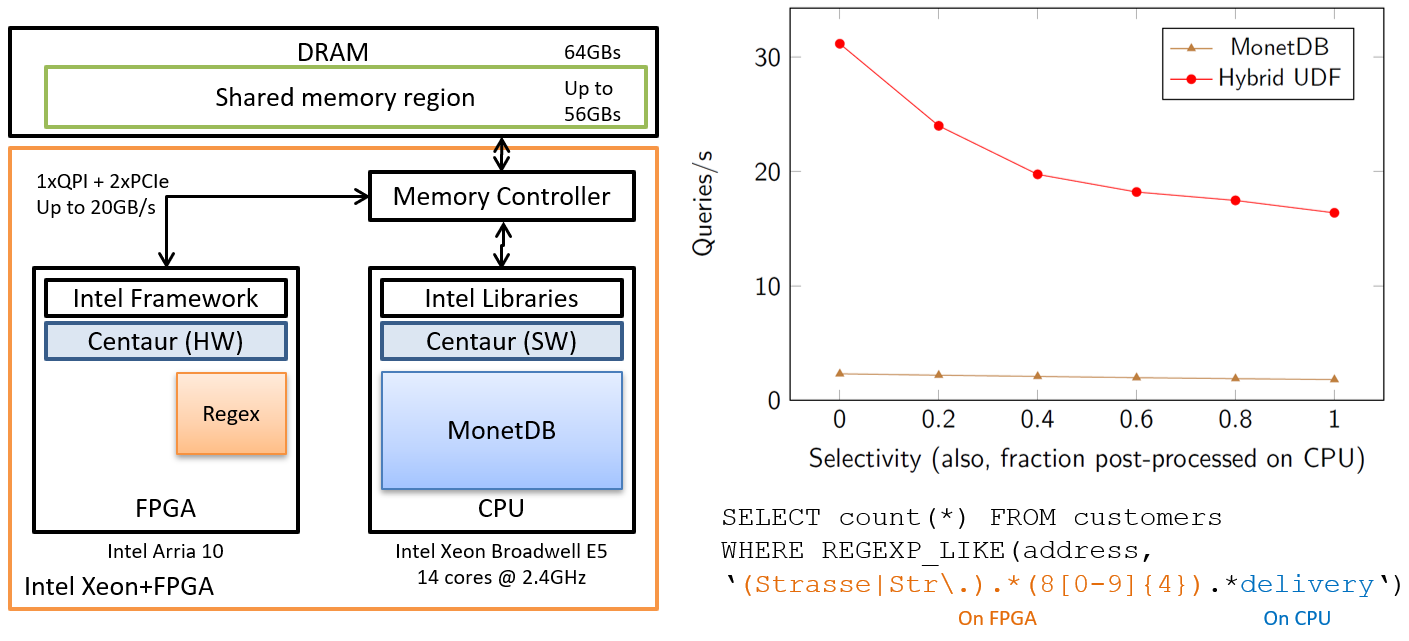
\includegraphics[width=0.9\linewidth]{hybrid-exec.png}
\caption{Even if only part of the regular expression fits on the FPGA it is worth to offload it because the post-processing becomes cheaper, resulting in an overall faster execution.\label{fig:hybrid-regex}}
\end{figure}

The regular expression-based LIKE operator that we implemented in MonetDB~\cite{sidler-regex-sigmod17} running on top of the Intel Xeon+FPGA platform is another example of the hybrid operator methodology. If the expression can't be encoded in its entirety on the FPGA, because, for instance, it contains too many characters (such as the bottom example in Figure~\ref{fig:hybrid-regex}), we cut it at the last possible wildcard and process the first part of the expression on the FPGA and the second part in software. For each string, the FPGA operator returns an index that signifies the end of the location where the regular expression matched the string. The software can pick up processing from this point in case of hybrid processing and match the rest of the expression. In case the entire expression fits on the FPGA, however, the software has no additional work to do. In Figure~\ref{fig:hybrid-regex} we illustrate how, when compared to a single-threaded execution in MonetDB, the hybrid solution is always faster than the software-only one (for more details see~\cite{sidler-regex-sigmod17}). 

One aspect that makes the integration of programmable hardware in databases challenging is the change in the predictability of query runtimes. Therefore, in our work we aim to design circuits whose throughput is not affected by the problem instance they work on. This way the query optimizer can predict the rate at which data will be processed/filtered on the FPGA and with this information it can reliably decide when to offload. One example of such a design is the regular expression module we presented above. Since the overhead of compiling regular expressions to circuits and then performing partial reconfiguration (PR) could take longer than executing an entire query, we took a different approach: we created a ``universal'' automaton that could implement any expression, within some limits on the number of distinct characters to detect and the number of states. Small on-chip memories are used to describe the state machine and the characters of the regular expression, and their contents can be loaded at runtime in nanoseconds. We laid out this state machine as a pipeline, that processes one character per clock cycle, regardless of the contents of the on-chip memories. The conversion from a regular expression written by a user to the configuration parameters is performed in software but is orders of magnitude cheaper than circuit synthesis.


\section{The Road that Lies Ahead}

\subsection{Managing Programmable Hardware}

%\begin{tcolorbox}
\emph{How to best integrate hardware that, even though reprogrammable, will never be as flexible as software?}\\
\emph{Should the operating system/hypervisor control it, or can we build future databases that do this?}
%\end{tcolorbox}
\smallskip

Even though there are efforts in the FPGA community to speed up the process of partial reconfiguration, it is unlikely that the overhead of this operation will ever be as small as that of a software context switch. As a result, databases must find ways to adapt to the idea of running on specialized hardware that, even though, can be reprogrammed, doesn't have the flexibility of software. The main question that needs to be answered in this space is who will ``own'' the acceleration functionality, because this also defines whether the database needs only to be able to compile its queries to take advantage of the accelerators, or whether it could also synthesize fully custom accelerators depending on the workload.

If it is the OS/hypervisor that controls the accelerator, then the database still has to be able to adapt to different underlying hardware acceleration functionality, that will likely be both designed and managed by the infrastructure/cloud provider. In this scenario, the database has to create query plans that take advantage of the specific machine's acceleration opportunities. For this, it is likely that we can reuse techniques that are already present in databases for compiling code for different target CPU features such as SIMD units~\cite{pirk-compiler-cidr19}.

Alternatively, if the database takes full ownership of the accelerator, it will have more responsibility but also greater opportunities. Instead of relying on the cloud provider to design general-purpose acceleration units that might or might not match the database's needs, the database developer can design and synthesize the right ones and integrate them tighter with the database. What's more, the database could even generate and synthesize workload-specific accelerators at runtime.

In DoppioDB~\cite{owaida-centaur-fccm17}\cite{sidler-doppiodb-sigmod17} we explored the case where the database manages the accelerator. The role of the operating system is to set up a basic infrastructure on the FPGA, configuring it with several ``slots'' that can be filled in using partial reconfiguration (we call these slots hardware threads because the interface to them in software is similar to a function call on a new thread). Once the database has started, the FPGA gets access to the process's virtual memory space and the database can explicitly manage what tasks the different slots perform, choosing in our prototype from a small library of available operators. In DoppioDB, instead of focusing only on the usual SQL operators like selection or joins, we began exploring how one could extend what the database is capable of, targeting machine learning type of operators, such as training a model using stochastic gradient descent or running inference with decision trees. This functionality was exposed using a UDF mechanism, but in the future could be integrated much tighter with the database. The research question that emerges is how to populate the hardware operator library and what granularity these operators should have. Recent work by Kara et al.~\cite{kara-join-sigmod17} shows that it is possible to offload sub-operators successfully to the FPGA. However, the identification of generic enough sub-operators that can be deployed on an accelerator and parameterized/composed at runtime remains an open challenge.

\subsection{Compilation/Synthesis for Programmable Hardware}


%\begin{tcolorbox}
\emph{Are there reusable building blocks that would make query compilation easier for programmable hardware?}\\
\emph{Should databases have their own DSLs from which to generate hardware accelerators?}
\smallskip
%\end{tcolorbox}

The second big question is how to express acceleration functionality for database use-cases in an efficient way. As opposed to CPUs or GPUs where the architecture (ISA, caches, etc.) is fixed, in an FPGA it is not. This adds a layer of complexity to the problem of compiling operators, as well as query planning in general. 
Given even just the heterogeneity of modern CPUs and their different SIMD units, there is already a push for databases to incorporate more and more compiler ideas~\cite{pirk-compiler-cidr19}\cite{pirk-voodoo-vldb16}. 

The side effect of bringing more ideas from compilers into databases is that it will likely also be easier to integrate DSLs for hardware accelerators~\cite{sycl2016}\cite{koeplinger-spatial-pldi18}\cite{maxcompiler} into the database. However, many of these solutions are targeting compute kernels written in languages such as OpenCL~\cite{sycl2016}, that are a better fit for HPC and machine learning type functionality than database operations. Therefore, novel ideas are needed that bridge the space between databases and languages/compilers for specialized hardware. One possible direction to explore is related to the design of the Spatial language and compiler~\cite{koeplinger-spatial-pldi18}. Spatial approaches the problem of writing parallel code for accelerators in a way that accounts for the fact that circuits are physically laid out on the chip. Given that query plans are often composed by a set of sub-operators that are parameterized differently to implement, for instance, different join types, these could be an intermediate step between SQL and hardware circuit that allows the database to offload a pipeline of such sub-operators to the FPGA in an automated manner.

Another aspect that makes translating operators to hardware-based accelerators challenging comes from the fact that not all functionality will fit on the device.  This is true regardless whether we target an FPGA, a P4-based switch or SmartNIC, or an ASIC-based solution such as the DAX. Therefore, even if the best case of an operator can be efficiently translated to hardware, corner cases will have to be handled without significantly impacting performance. For this reason, the challenge of compilation is also related to the ideas discussed before around hybrid execution and query planning. Frameworks that compile queries to such platforms will have to provide software-based post-processing functionality to ensure that corner cases are gracefully handled. The challenge in this hybrid computation is to find suitable points where to split the functionality in an automated way.

\section{Conclusion}

In this paper we made the case that the use of specialized hardware in analytical databases has a positive outlook, even though it has been approached pessimistically for a long time. To support this argument, we discussed the past and future challenges of including a specific kind of hardware accelerator, namely FPGAs, in databases. 

To address fears that deploying FPGAs always brings high overheads that reduce their ``raw'' speedup, we highlighted how, in today's distributed database landscape, they can be used to reduce bottlenecks of data movement by positioning them in data-path. Since they can process data at the rate at which it is retrieved from the data source, they never slow down data access, even if there is no opportunity for acceleration. We also discussed the opportunities that novel machine learning workloads bring. Their operators are typically compute bound on CPUs and using FPGAs we can achieve significant speedups even when compared to an entire socket with multiple cores. Finally, to demonstrate that it is possible to design FPGA-based operators that behave gracefully even if the entire functionality of the operator doesn't fit on the device, we discussed two examples from our previous work that implement hybrid computation across FPGA and CPU (a group-by operator and a regular expression matcher).

We also identify two areas in which significant progress has to be made for the inclusion of heterogeneous hardware in databases to become truly widespread. One is finding ways to actively manage the programmable hardware underneath the database, shaping it to workloads using partial reconfiguration and parameterizable circuits. The second question is about finding the right programming primitives for hardware accelerators in the context of database operators, to avoid designing from scratch each new accelerator idea and to allow the database to offload parts of a query more flexibly at runtime. It is unlikely that we can provide answers for both questions only from inside the database community and will have to instead collaborate with researchers working in the areas of operating systems, programming languages and compilers.

\small
\section*{Acknowledgments}

Our cited work and many of the lessons learned are a result of the author's collaboration with current and past members of the Systems Group at ETH Z\"{u}rich, in particular, Gustavo Alonso, David Sidler, Louis Woods and Jana Giceva.


\begin{thebibliography}{10} 
\itemsep=1pt 

\bibitem{banerjee-databasemachine-79} J. Banerjee, D. Hsiao and K. Kannan. \newblock DBC: A Database Computer for Very Large Databases. \newblock \emph{IEEE Transactions on Computers}, 6, pp. 414-429, IEEE, 1979.

\bibitem{dewitt-gamma-1990} D.J. DeWitt, S. Ghandeharizadeh, D.A. Schneider, A. Bricker, H.I. Hsiao, R. Rasmussen. \newblock The Gamma database machine project. \newblock \emph{IEEE Transactions on Knowledge and data engineering}, 2(1), pp. 44-62, 1990.

\bibitem{francesco-netezza-2011} P. Francisco. \newblock The Netezza data appliance architecture: A platform for high performance data warehousing and analytics. \newblock \emph{IBM Red Books}, 2011.

\bibitem{wu-q100-asplos14} L. Wu, A. Lottarini, T.K. Paine, M. Kim, K.A. Ross \newblock Q100: The Architecture and Design of a Database Processing Unit. \newblock \emph{ASPLOS'14}, pp. 255-268, 2014.

\bibitem{agrawal-rapid-17} S.R. Agrawal, S. Idicula, A. Raghavan, E. Vlachos, V. Govindaraju, V. Varadarajan, E. Sedlar et al. \newblock A many-core architecture for in-memory data processing. \newblock \emph{MICRO'17}, pp. 245-258, ACM, 2017.

\bibitem{esmaeilzadeh-darksilicon-isca11} H. Esmaeilzadeh, E. Blem, R.S. Amant, K. Sankaralingam and D. Burger. \newblock Dark silicon and the end of multicore scaling. \newblock \emph{ISCA'11}, pp. 365-376, IEEE, 2011. 

\bibitem{sato-tpu-google17} K. Sato, C. Young, D. Patterson. \newblock An in-depth look at Google’s first Tensor Processing Unit (TPU). \newblock \emph{Google Cloud Big Data and Machine Learning Blog, 12}, 2017.

\bibitem{firestone-catapult-nsdi18} D. Firestone, A. Putnam, S. Mundkur, D. Chiou, A. Dabagh, et al. \newblock Azure Accelerated Networking: SmartNICs in the Public Cloud. \newblock \emph{NSDI'18}, USENIX, 2018.

\bibitem{gupta-harp-fpl16} P.K. Gupta. \newblock Accelerating datacenter workloads. \newblock \emph{FPL'16}, 2016.

\bibitem{mahajan-danafpga-vldb18} D. Mahajan, J.K. Kim, J. Sacks, A. Ardalan, A. Kumar, H. Esmaeilzadeh. \newblock In-RDBMS Hardware Acceleration of Advanced Analytics. \newblock \emph{Proceedings of the VLDB Endowment}, 11(11), 2018.

\bibitem{hellerstein-madlib-vldb12} J.M. Hellerstein, C. Re, F. Schoppmann, D.Z. Wang, E. Fratkin, A. Gorajek, K.S. Ng, C. Welton, X. Feng, K. Li,et al. \newblock The MADlib analytics library: or MAD skills, the SQL. \newblock \emph{PVLDB}, 5(12), pp. 1700–1711, 2012.

\bibitem{kraska-sage-cidr19} T. Kraska, M. Alizadeh, A. Beutel, E. Chi, J. Ding, A. Kristo, V. Nathan, et al. \newblock SageDB: A learned database system. \newblock \emph{CIDR'19}, 2019.

\bibitem{sitaridi-gpuregex-2016} E. Sitaridi, K. Ross. \newblock GPU-accelerated string matching for database applications. \newblock \emph{Proceedings of the VLDB Endowment}, pp. 719-740, 2016.

\bibitem{sukhwani-dbanalyitcs-ieee14} B. Sukhwani, H. Min, M. Thoennes, P. Dube, B. Brezzo, S. Asaad, D.E. Dillenberger. \newblock \emph{Database analytics: A reconfigurable-computing approach}, IEEE Micro, 34(1), pp. 19-29, 2014.

\bibitem{oskin-active-ieee98} M. Oskin, F.T. Chong, T. Sherwood. \newblock Active pages: A computation model for intelligent memory. \newblock \emph{IEEE Computer Society}, Vol. 26, No. 3, pp. 192-203, 1988.

\bibitem{koo-summarizer-micro17} G. Koo, K.K. Matam, H.V. Narra, J. Li, H.W. Tseng, S. Swanson, M. Annavaram. \newblock Summarizer: trading communication with computing near storage. \newblock \emph{MICRO'17}, pp. 219-231, ACM, 2017.

\bibitem{jo-yoursql-vldb16} I. Jo, D.H. Bae, A.S. Yoon, J.U. Kang, S. Cho, D. Lee, J. Jeong. \newblock YourSQL: a high-performance database system leveraging in-storage computing. \newblock \emph{Proceedings of the VLDB Endowment}, 9(12), pp. 924-935, 2016.

\bibitem{woods-Ibex-vldb14} L. Woods, Z. Istvan, G. Alonso. \newblock Ibex: an intelligent storage engine with support for advanced SQL offloading. \newblock \emph{Proceedings of the VLDB Endowment}, 7(11), pp. 963-974, 2014.

\bibitem{jun-bluedbm-tocs16} S.W. Jun, M. Liu, S. Lee, J. Hicks, J. Ankcorn, M. King, S. Xu. \newblock BlueDBM: Distributed Flash Storage for Big Data Analytics. \newblock \emph{ACM TOCS} 34(3), 7, 2016.

\bibitem{barthels-join-sigmod15} C. Barthels, S. Loesing, G. Alonso, D. Kossmann. \newblock Rack-scale in-memory join processing using RDMA. \newblock \emph{SIGMOD'15}, pp. 1463-1475, ACM, 2015.

\bibitem{dragojevic-farm-debull17} A. Dragojevic; D. Narayanan; M. Castro. \newblock RDMA Reads: To Use or Not to Use?. \newblock \emph{IEEE Data Eng. Bull.}, vol. 40, no 1, pp. 3-14, 2017.

\bibitem{bosshart-p4-comrew14} P. Bosshart, D. Daly, G. Gibb, M. Izzard, N. McKeown, J. Rexford, et al. \newblock P4: Programming protocol-independent packet processors. \newblock \emph{ACM SIGCOMM Computer Communication Review}, 44(3), pp. 87-95, 2014.

\bibitem{aingaran-dax-hcs16} K. Aingaran, S. Jairath, D. Lutz. \newblock Software in Silicon in the Oracle SPARC M7 processor. \newblock \emph{Hot Chips Symposium (HCS'16)}, pp. 1-31, IEEE, 2016.

\bibitem{teubner-fpgabook-2011} J. Teubner and L. Woods. \newblock Data processing on FPGAs. \newblock \emph{Synthesis Lectures on Data Management}, 5(2), pp. 1-118, 2011.

\bibitem{casper-fpgaacceldb-fccm14} J. Casper, K. Olukotun. \newblock Hardware acceleration of database operations. \newblock \emph{FPGA'14}, pp. 151-160, ACM, 2014.

\bibitem{dennl-sqlaccel-fccm13} C. Dennl, D. Ziener, J. Teich \newblock Acceleration of SQL restrictions and aggregations through FPGA-based dynamic partial reconfiguration. \newblock \emph{FCCM'13}, pp. 25-28, IEEE, 2013.

\bibitem{boncz-x100-cidr05} P.A. Boncz, M. Zukowski, N. Nes. \newblock MonetDB/X100: Hyper-Pipelining Query Execution. \newblock \emph{CIDR}, Vol. 5, pp. 225-237, 2005.

\bibitem{klimovic-flash-eurosys16} A. Klimovic, C. Kozyrakis, E. Thereska, B. John, S. Kumar. \newblock Flash storage disaggregation. \newblock \emph{EUROSYS'16}, 2016.

\bibitem{fang-udp-micro17} Y. Fang, C. Zou, A.J. Elmore, A.A. Chien. \newblock UDP: a programmable accelerator for extract-transform-load workloads and more. \newblock \emph{MICRO'17}, pp. 55-68, ACM, 2017.

\bibitem{istvan-caribou-vldb17} Z. Istvan, D. Sidler, G. Alonso. \newblock Caribou: intelligent distributed storage. \newblock \emph{Proceedings of the VLDB Endowment}, 10(11), pp. 1202-1213, 2017.

\bibitem{zistvan-diss-2018} Z. Istvan. \newblock Building Distributed Storage with Specialized Hardware \newblock Doctoral dissertation, ETH Zurich, 2018.

\bibitem{owaida-centaur-fccm17} M. Owaida, D. Sidler, K. Kara, G. Alonso \newblock Centaur: A framework for hybrid CPU-FPGA databases. \newblock \emph{FCCM'17}, pp. 211-218, IEEE, 2017.

\bibitem{owaida-trees-fpl17} M. Owaida, H. Zhang, C. Zhang, G. Alonso. \newblock Scalable inference of decision tree ensembles: Flexible design for CPU-FPGA platforms. \newblock \emph{FPL'17}, IEEE, 2017.

\bibitem{umuroglu-finn-fpga17} Y. Umuroglu, N.J. Fraser, G. Gambardella, M. Blott, P. Leong, M. Jahre, K. Vissers. \newblock Finn: A framework for fast, scalable binarized neural network inference. \newblock \emph{FPGA'17}, pp. 65-74, ACM, 2017.

\bibitem{sidler-regex-sigmod17} D. Sidler, Z. Istvan, M. Owaida, G. Alonso. \newblock Accelerating pattern matching queries in hybrid CPU-FPGA architectures. \newblock \emph{SIGMOD'17}, pp. 403-415, ACM, 2017.

\bibitem{sidler-doppiodb-sigmod17} D. Sidler, Z. Istvan, M. Owaida, K. Kara, G. Alonso. \newblock doppioDB: A hardware accelerated database. \newblock \emph{SIGMOD'17}, pp. 1659-1662, ACM, 2017.

\bibitem{sycl2016} M. Wong, A. Richards, M. Rovatsou, R. Reyes. \newblock Khronos's OpenCL SYCL to support heterogeneous devices for C++, 2016.

\bibitem{koeplinger-spatial-pldi18} D. Koeplinger, M. Feldman, R. Prabhakar, Y. Zhang, S. Hadjis, R. Fiszel, K. Olukotun. \newblock Spatial: a language and compiler for application accelerators. \newblock \emph{PLDI'18}, pp. 296-311, ACM, 2018.

\bibitem{maxcompiler} O Mencer. \newblock Maximum performance computing for Exascale applications. \newblock \emph{ICSAMOS'12}, 2012.

\bibitem{pirk-compiler-cidr19} H. Pirk, J. Giceva, P. Pietzuch. \newblock Thriving in the No Man’s Land between Compilers and Databases. \newblock \emph{CIDR}, 2019.

\bibitem{pirk-voodoo-vldb16} H. Pirk, O. Moll, M. Zaharia, S. Madden \newblock Voodoo - A vector algebra for portable database performance on modern hardware. \newblock \emph{Proceedings of the VLDB Endowment}, 9(14), pp. 1707-1718, 2016.

\bibitem{kara-join-sigmod17} K. Kara, J. Giceva, G. Alonso. \newblock Fpga-based data partitioning \newblock \emph{SIGMOD'17}, pp. 433-445, ACM, 2017.

\end{thebibliography} 

\end{document}

\end{article}

\begin{article}
{Scheduling Data-Intensive Tasks on Heterogeneous Many Cores}
{P{\i}nar T\"oz\"un, Helena Kotthaus}
\graphicspath{{submissions/ptozun/figs/}}
\documentclass[11pt]{article} 

\usepackage{deauthor,times,graphicx}
\usepackage{url}
\usepackage{subfig}

%\graphicspath{{authorname/}}

%\newcommand{\reffig}[1]{Figure~\ref{fig:#1}}
%\newcommand{\refsec}[1]{Section~\ref{sec:#1}}
%\newcommand{\reftab}[1]{Table~\ref{tab:#1}}

\begin{document}

\newcommand{\reffig}[1]{Figure~\ref{fig:#1}}
\newcommand{\refsec}[1]{Section~\ref{sec:#1}}
\newcommand{\reftab}[1]{Table~\ref{tab:#1}}

\title{Scheduling Data-Intensive Tasks on Heterogeneous Many Cores}

\author{P{\i}nar T\"oz\"un \\ IT University of Copenhagen \\ \texttt{pito@itu.dk}
\and Helena Kotthaus \\ TU Dortmund University \\ \texttt{helena.kotthaus@tu-dortmund.de}}

\maketitle

\begin{abstract}

Scheduling various data-intensive tasks over the processing units of a server
has been a heavily studied but still challenging effort.
In order to utilize modern multicore servers well,
a good scheduling mechanism has to be conscious of different dimensions of parallelism offered by these servers.
%both the vertical and horizontal parallelism offered by these servers.
This requires being aware of the micro-architectural features of processors,
the hardware topology connecting the processing units of a server,
and the characteristics of these units as well as the data-intensive tasks.
The increasing levels of parallelism and heterogeneity in emerging server hardware
amplify these challenges in addition to the increasing variety of data-intensive applications.

This article first surveys the existing scheduling mechanisms targeting
the utilization of a multicore server with uniform processing units. 
Then, it revisits them in the context of emerging server hardware composed of many diverse cores
and identifies the main challenges.
Finally, it concludes with the description of a preliminary framework targeting these challenges.
Even though this article focuses on data-intensive applications on a single server,
many of the challenges and opportunities identified here are not unique to such a setup,
and would be relevant to other complex software systems as well as
resource-constrained or large-scale hardware platforms. 

\end{abstract}

\section{Introduction}
\label{sec:intro}

% why scheduling
Utilizing the processors of commodity servers well is crucial to avoid wasting
resources, energy, and money in data centers regardless of their scale \cite{Hamilton10}.
As a result, quest to remove the bottlenecks of data management systems causing underutilization
of modern commodity servers have been the focus of many past and ongoing work \cite{AilamakiLTPP17}.
One of the essential challenges in this quest is scheduling various data-intensive tasks
effectively over the processing units that are available to these tasks. 
The fundamental evolution of the server hardware and the increasing variety
of the data-intensive applications over the recent years amplify this challenge.

\begin{figure}
\subfloat[\label{fig:hw}]{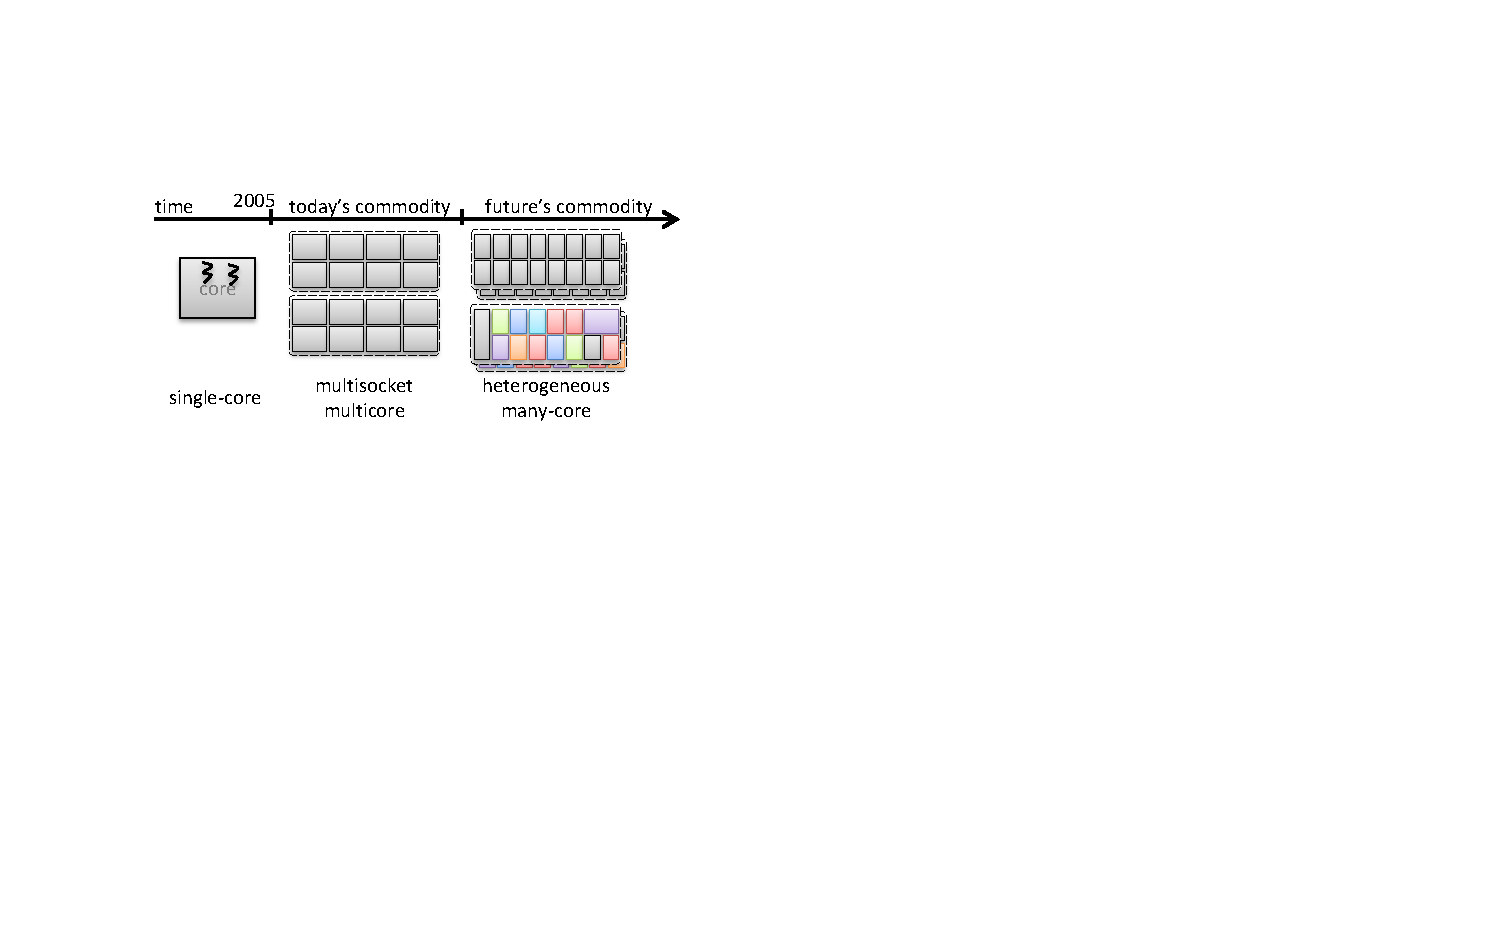
\includegraphics[width=0.6\textwidth]{fig-hw.pdf}}
\hfill
\subfloat[\label{fig:dia}]{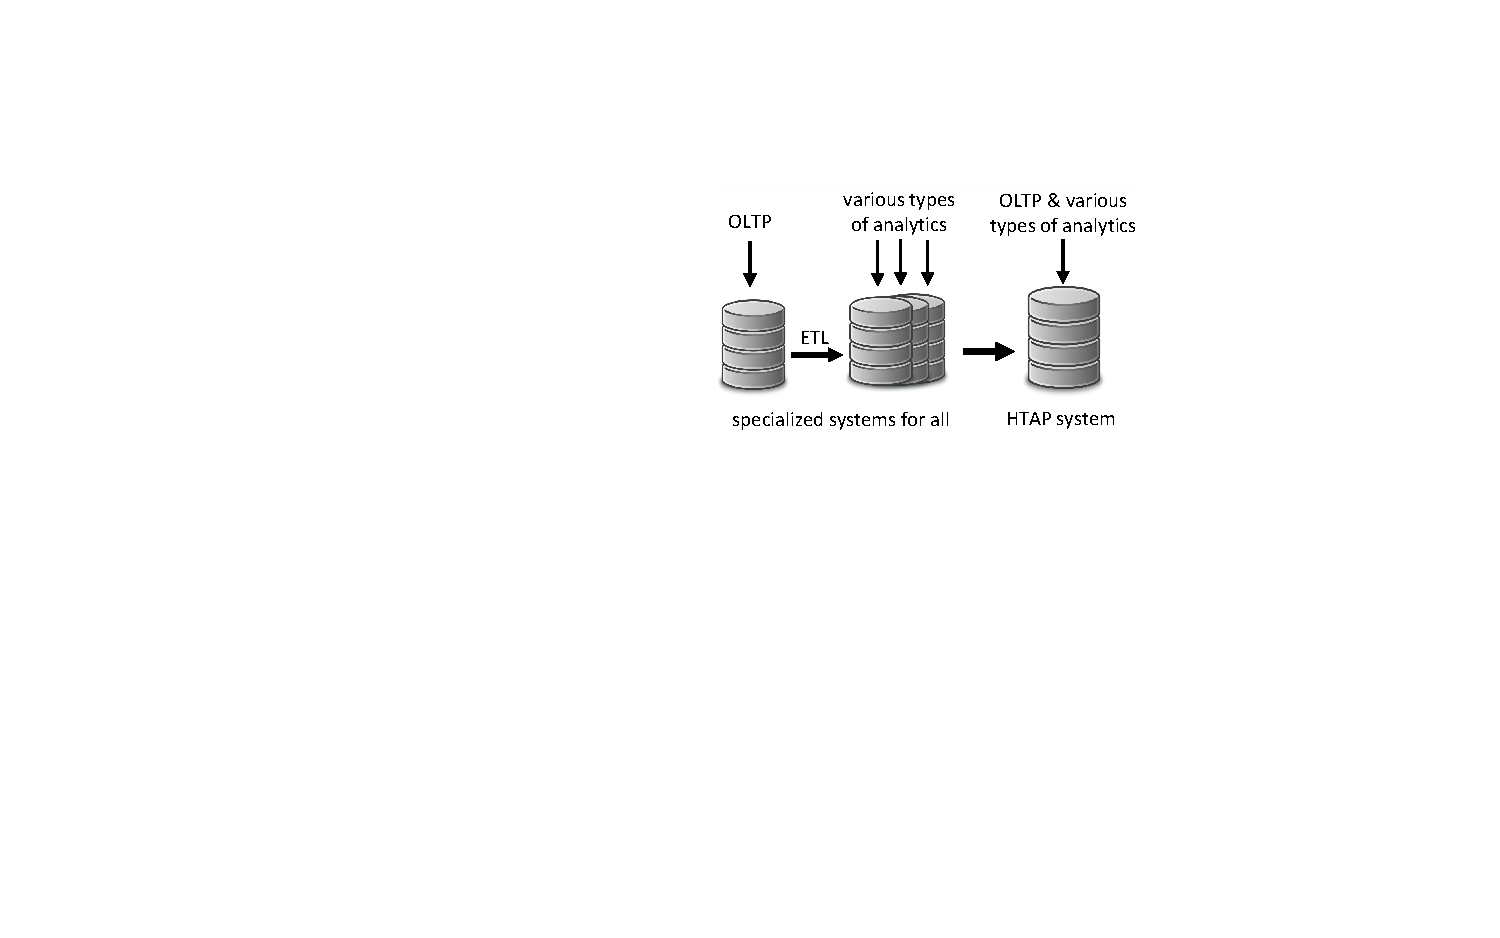
\includegraphics[width=0.4\textwidth]{fig-dia.pdf}}
\caption{(a) Evolution of server hardware over time following Moore’s Law and Dennard Scaling.
Each break in the timeline represents a disruptive period for processor evolution due to power concerns.
(b) Ways to deploy data-intensive applications.}
\label{fig:hwdia}
\end{figure}

% the server hardware gives us different types of parallelism ... in one paragraph and picture maybe
Server hardware has gone through major advances over the years as illustrated in \reffig{hw}.
These advances have stemmed from Moore’s Law \cite{Moore65},
which is the observation that the number of transistors in a dense integrated circuit doubles approximately every two years.
To exploit the increase in the transistor counts in a unit area, initially,
computer architects focused on boosting the performance of a single core while designing chips
(left-hand side of \reffig{hw}).
Around 2005, however, Dennard Scaling \cite{DennardGYRBAL74},
which states that as the transistors get smaller their power density in a unit area remains constant, came to a halt.
Increasing the complexity of a processor core became non-viable since it raised concerns about power draw and heat dissipation.
To overcome this limitation, computer architects started to add more and more cores on a single processor \cite{OlukotunNHWC96}
and more and more processors in servers (middle part of \reffig{hw}).
Multicore processors have enabled the continuation of Moore’s Law despite the halt of Dennard Scaling.
Unfortunately, the limits of the traditional multicore processor design is also upon us. 
Adding more and more cores to a processor cannot be the only path to overcome the halt of Dennard Scaling
since we will not be able to power all of those cores up simultaneously.
This trend is also known as dark silicon \cite{EsmaeilzadehBASB11}.
To overcome this limitation, we must design cores that are more energy-efficient.
One way to achieve this by specializing cores, reducing energy spent per instruction, for certain tasks \cite{HennessyP19}.
Then, as part of the commodity servers, one can utilize the specialized cores in addition to the general-purpose ones.
%which forces us to commoditize alternatives to general-purpose processors
%to optimize energy spent per instruction \cite{HennessyP19}.
The emerging server hardware landscape, therefore,
will likely to be composed of a heterogeneous set of processing units
(as illustrated by the different colors in right-hand side of \reffig{hw});
each specialized to execute a specific task very well,
with opportunities for extreme levels of parallelism.

% variety of applications 
In parallel to the evolution of commodity server hardware that data-intensive applications typically run on,
the applications themselves and how they are deployed have also changed over time as illustrated in \reffig{dia}. 
Transaction and analytical processing used to be the two broad categories of data-intensive applications.
Analytics, in turn, have several distinct sub-categories such as
online analytical processing, data warehousing, machine learning, graph analytics, etc.
Traditionally, they have been deployed separately and data moved from an operational system
(such as an online transaction processing system)
to various types of analytics systems using an extract-transform-load (ETL) process. 
The reason for this separation is that optimal system design for serving
transactional and different types of analytical tasks are different
(e.g., row stores for OLTP, column stores for OLAP, NoSQL for unstructured data, etc.).
In recent years, however, the popularity of the data-intensive applications such as 
real-time inventory/pricing/recommendations, fraud detection, risk analysis, IoT, AI, etc.
require data management systems that can run fast transactions and analytics simultaneously.
As a result, there is an increasing demand for data management systems that can handle
hybrid transactional and analytical processing (HTAP) efficiently \cite{OzcanTT17}.

% the purpose of this text is to survey scheduling methods and challenges in three parts of this picture 
Designing a scheduling mechanism that is able to leverage the heterogeneity of
processing units for the variety of the data-intensive tasks to be executed
in the emerging hardware and software landscapes is a difficult but significant challenge to tackle. 
The goal of this article is to derive some guidelines to overcome this challenge
in the context of a single node of commodity server hardware.
First, \refsec{sched}
surveys some of the existing work that target scheduling of data-intensive tasks on modern homogeneous multicore servers.
Then, \refsec{het} discusses emerging heterogeneous server hardware landscape and
considers existing work in the context of such hardware.
Finally, \refsec{guide}
illustrates a framework for scheduling diverse set of (or hybrid) data-intensive tasks
over diverse set of (or heterogeneous) processing units focusing on the resource estimation challenges.

\section{Scheduling Data-Intensive Tasks over Different Dimensions of Parallelism}
\label{sec:sched}

As previously mentioned,
we view the effective scheduling of different data-intensive tasks as a significant factor
when it comes to effective utilization of the resources of modern server hardware.
Any mechanism that targets effective scheduling must be able to answer the following questions. 

\textit{\textbf{What} to schedule?}
This question determines the unit of scheduling.
What is the granularity of the task to be executed on a specific processing unit?
Is it the whole data-intensive task required by a client request or is it part of it?
If it is a part of it, what is the size of that part?

\textit{\textbf{Where} to schedule?}
This challenge handles the mapping between tasks and processing units.
This mapping has both a \textit{static} and a \textit{dynamic} part.
The static mapping targets the question of what the most effective processing unit/units to execute a task is/are.
The answer to this question assumes that every kind of processing unit is available in infinite amounts.
In practice, however, we rarely have all kinds of processing units in a single server and the hardware resources are finite.
The dynamic mapping must consider the question of whether the ideal processing units
for a task are available at the exact time that we have to execute that task.
In addition, in the case of unavailability, what are the next best alternatives?

\textit{\textbf{How} to schedule?}
This challenge provides the necessary execution and communication primitives,
especially if multiple processing units are involved in executing a task.
What are the primitives to utilize while scheduling a task or parts of a task?
Which level(s) of the system stack these primitives come from? 

The following subsections survey the scheduling mechanisms proposed in recent work that
depart from the conventional wisdom when it comes to the answers to the questions above.
\refsec{sched:impl} and \refsec{sched:expl} focus on utilizing the resources of
a single core and multiple uniform cores, respectively.

\subsection{Implicit/Vertical Parallelism}
\label{sec:sched:impl}

Before Dennard Scaling made it problematic to put more complexity within a core due to heat dissipation concerns,
exploiting Moore's Law meant boosting the performance of a single core.
This resulted in parallelism opportunities within a core through techniques like
instruction level parallelism, pipelining, out-of-order execution, simultaneous multithreading, etc.
We refer to this kind of parallelism as \textit{implicit/vertical} parallelism
as the different tasks are time-multiplexed on the same core
instead of being run concurrently in the same execution cycle.
The main insight behind this kind of parallelism is overlapping various stall times with other work
instead of a core wasting the execution cycles being idle.
For example, as a core waits for fetching an instruction or data item from memory due to it not being present in L1 caches,
one can overlap this waiting time with another instruction or data fetch request from the same task
or execute another task on the same core.
In addition, mostly hardware manages this kind of parallelism and software has the luxury to be oblivious to it.
Therefore, before multicores emerged,
the software systems got faster with each new generation of servers without having to make fundamental design changes.

On the other hand, 
for many data-intensive applications being oblivious to implicit parallelism leads to severe underutilization of
the micro-architectural resources of servers.
Several workload characterization studies emphasize the high rates of memory access related stall times
due to either instruction or data accesses for data-intensive applications \cite{Ferdman+12, SirinTPA16}.
Similarly, techniques like simultaneous multithreading may even hurt performance if not used carefully \cite{ZhouCRS05}.
Multiple data-intensive tasks sharing the same resources in a core simultaneously may put more pressure on caches
due to their aggregate data and instruction footprint.
Therefore,
there is value to rethink the way we design and schedule data-intensive tasks even when utilizing implicit parallelism.

\begin{figure}
\centering
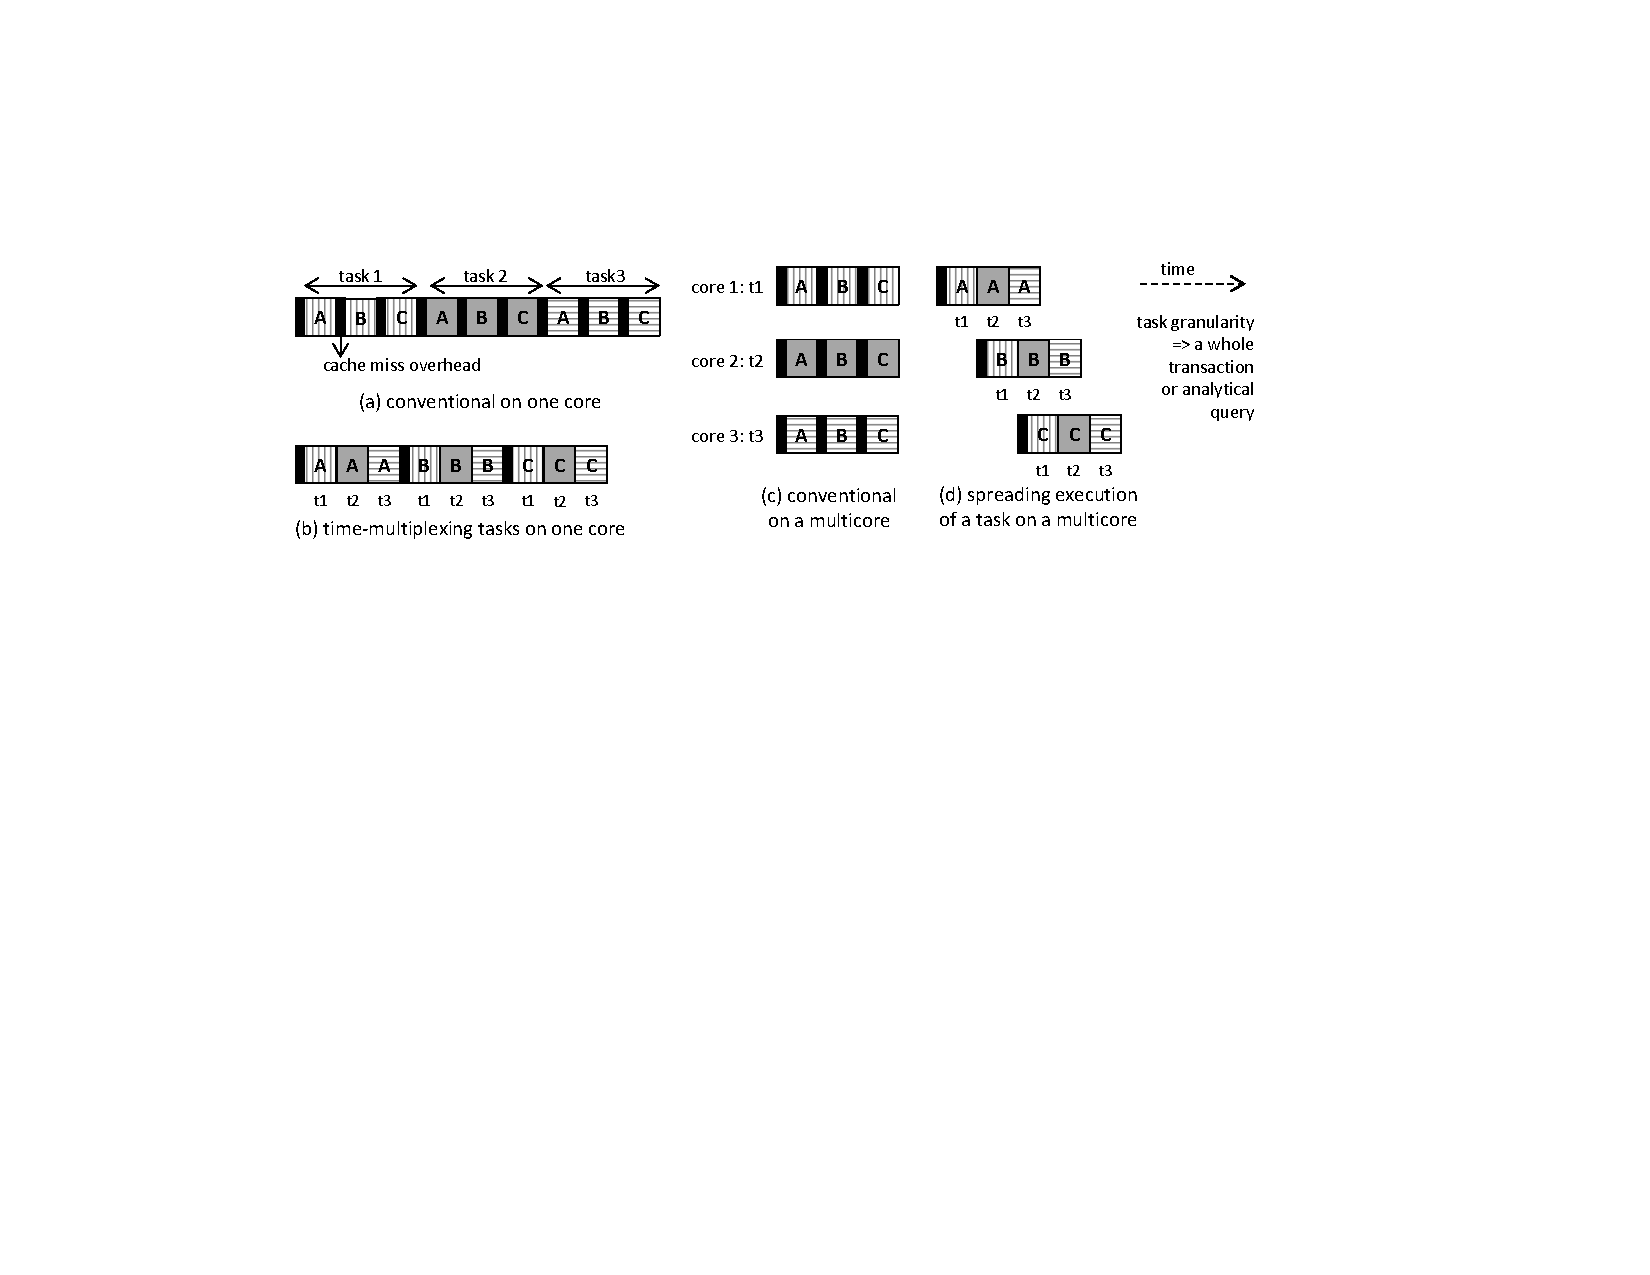
\includegraphics{fig-sched.pdf}
\caption{Different ways of scheduling data-intensive tasks.
%on one core (a \& b) and on a multicore (c \& d) assuming no context switching due to I/O.
In the context of this illustration a task is at the granularity of a transaction or an analytical query,
where A, B, and C are the sub-tasks of this task.}
\label{fig:sched}
\end{figure}

\reffig{sched} illustrates alternative ways of scheduling a data-intensive task
on a single core (a \& b) and on multiple cores (c \& d).
The figure assumes that tasks run over a setup that has fast I/O (e.g., DRAM, NVRAM, low-latency SSD)
and hence do not require context switching due to slow I/O (e.g., HDD).
%assuming the tasks can run without any context switching due to I/O.
In the figure, a data-intensive task is at the granularity of a whole transaction or analytical query.
The task has three sub-tasks A, B, C.
In the interest of our discussion, let's assume that these sub-tasks are at a granularity
where their instruction or data set sizes can fit in L1-I or L1-D, respectively.
This section discusses \reffig{sched}(a \& b) since the focus is on implicit parallelism,
whereas the discussion of \reffig{sched}(c \& d) is in \refsec{sched:expl}.

\reffig{sched}(a) depicts the more conventional way of scheduling tasks.
In this case, the tasks run without any interruptions on a core as a whole one after the other
based on their priority in a task queue in the system.
They take turns thrashing the caches since each executes sub-tasks A through
C in order independent of the other tasks.
Thus, each sub-task incurs overhead due to cache misses.
In this case,
the answer to the \textit{what} question is the whole task
while the \textit{where} question doesn't matter as there is only a single core,
and the answer to the \textit{how} question is mainly left to the default mechanisms
supported by the operating system.

\reffig{sched}(b) shows an alternative way to schedule the sub-tasks,
which time-multiplexes them with the goal of maximizing cache locality.
The first, \textit{lead}, task executes A incurring cache miss overhead as previously.
However, instead of proceeding to execute B, the first task context switches allowing,
in turn, the second and third tasks to execute instead.
The second and third tasks find sub-task A in L1 and thus incur no overhead due to misses.
Once all three tasks execute the first sub-task, execution proceeds to the second one and so on.

The core idea of time-multiplexing the tasks on a single core to improve cache locality
has been studied and shown to be effective in the context of both
instruction (L1-I) and data (L1-D) \cite{AttaTTAM13, HarizopoulosA04, HarizopoulosSA05, LarusP02} locality.
The main insight behind this idea is that similar tasks share common instructions or data or both.
As a result, they can benefit from constructive sharing of the cache resources to improve locality.
Fewer cache misses lead to better utilization of the micro-architectural resources
that enable implicit parallelism within a core
since a smaller portion of the overall execution time is spent on stalls. 
Even if a technique that focuses on instruction cache locality may hinder data cache locality or vice-versa,
the benefits of one may outshine the overhead of the other,
or the locality may improve at the higher levels of the cache hierarchy
despite the hindered L1 locality thanks to constructive sharing \cite{TozunAAM14}.

Achieving constructive sharing for different concurrent tasks in a system is not straightforward.
The first challenge is the underlying assumption of the tasks would have similar sub-tasks to be executed.
For data-intensive applications, this is not an issue.
No matter how different the output or high-level functionality of one data-intensive task from another,
data management or processing systems typically compose a subset of predefined sub-tasks to serve a task.
\reffig{common} and \reffig{intratask}
show some examples within the same or across different applications/tasks.
Transactions are composed of sub-tasks such as probing and scanning an index,
inserting a tuple to a table, updating a tuple, etc.
Traditional analytical queries are composed of projections, selections, joins, etc.
These sub-tasks themselves have common sub-tasks such as hash table lookup, data partitioning, sorting, etc.
across different types of sub-tasks or workloads.
There may be frequently accessed tables or indexes or metadata used by several of these sub-tasks.
Overall, there are many opportunities for constructive sharing in data-intensive applications.

Determining the granularity of sub-tasks to time-multiplex at runtime is a harder challenge
(to answer the \textit{what} question)
as well as orchestrating the runtime scheduling in a lightweight manner
(to answer the \textit{how} question).
Regarding the former challenge,
previous work either considers the granularity of database operators \cite{HarizopoulosSA05},
rely on monitoring the cache behavior at runtime
to determine when the L1 cache starts to become full \cite{AttaTTAM13},
or perform profiling \cite{HarizopoulosA04}.
Regarding the latter challenge,
previous work either adopts hardware mechanisms \cite{AttaTTAM13}
to sidestep the overheads of default context switching primitives of the operating system,
or develop specialized context switching at the kernel-level \cite{HarizopoulosA04}.

Finally, despite increasing the throughput,
time-multiplexing a batch of tasks on one core increases the average latency,
especially for the \textit{lead} task.
One has to take into account the priority or latency requirements of
the data-intensive tasks when deploying these types of scheduling mechanisms.
This challenge is definitely under-studied in the literature.

\begin{figure}
\centering
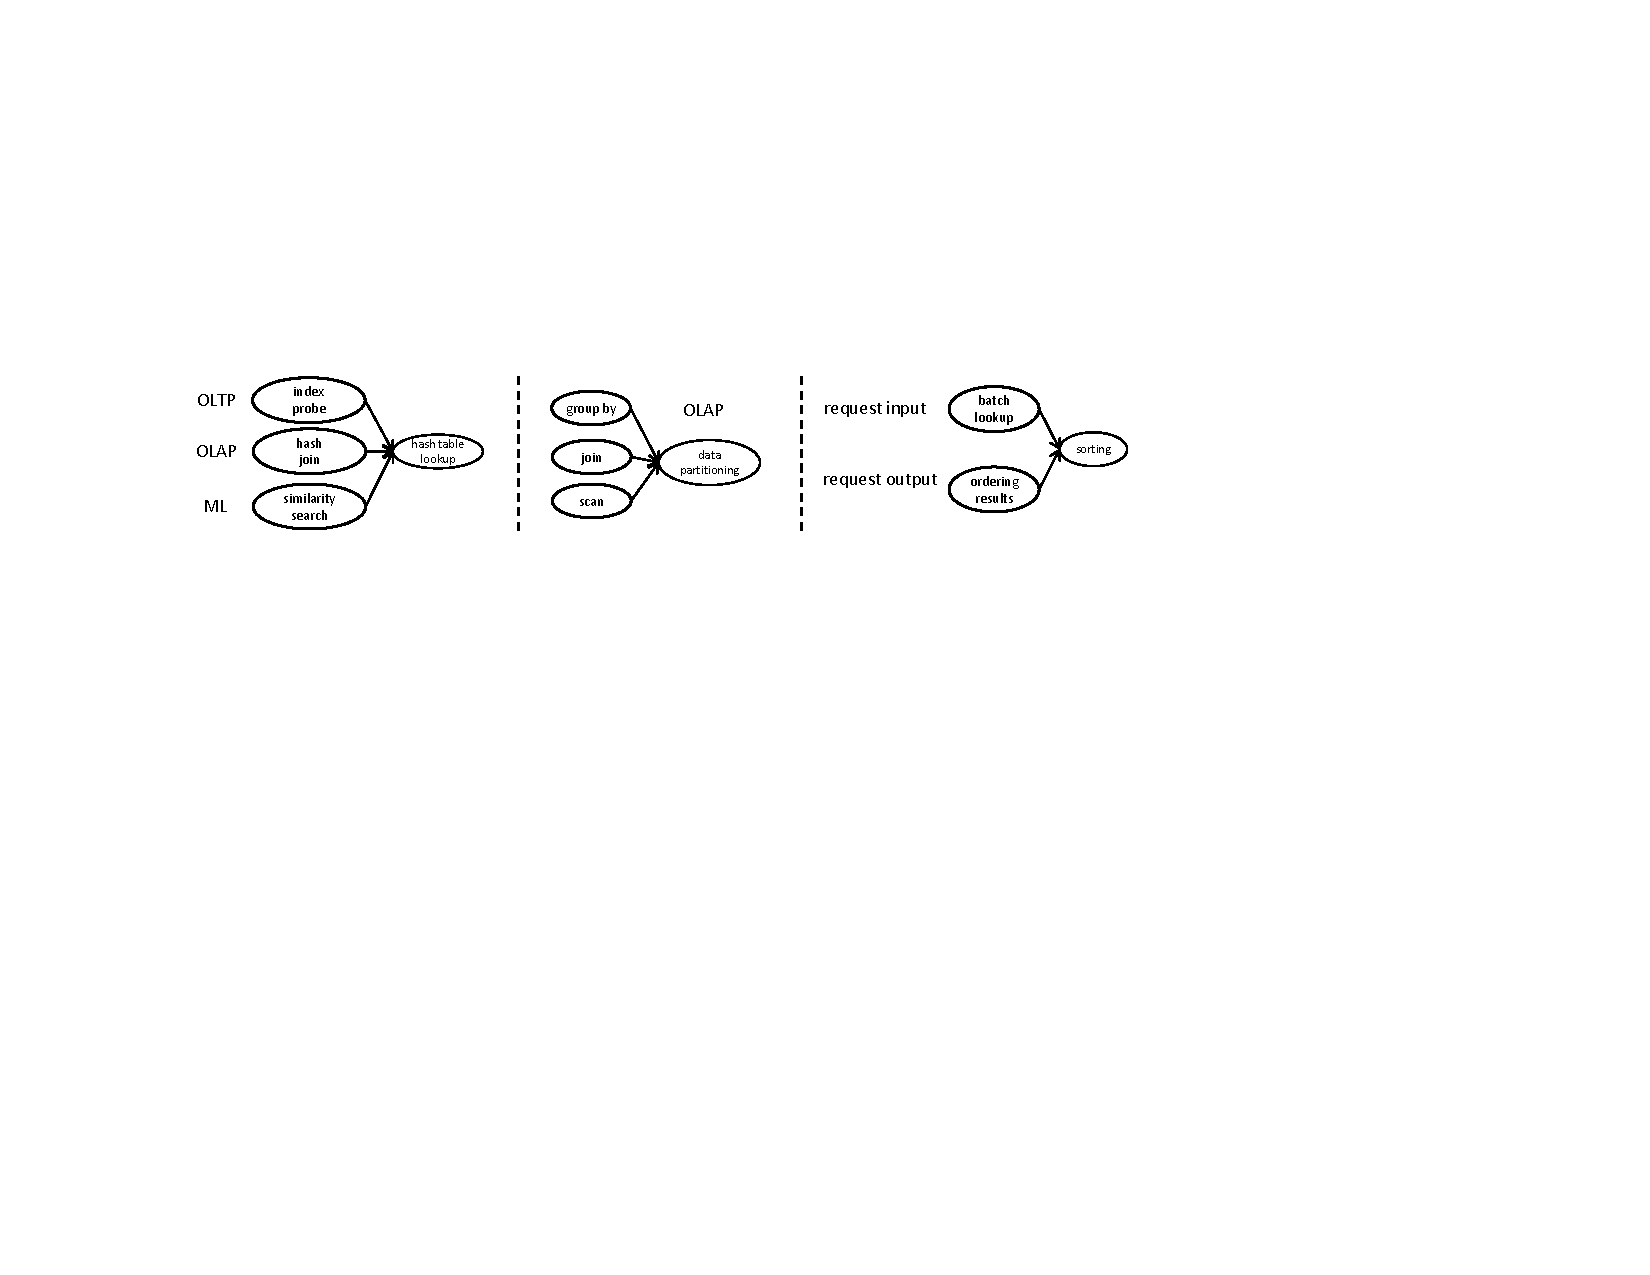
\includegraphics{fig-common.pdf}
\caption{Examples of common sub-tasks across different types of data-intensive applications.
Hash table lookup is common across OLTP, OLAP, and machine learning.
Data partitioning is common across many OLAP tasks.
Sorting is common both across data-intensive applications and
while ordering input/output values from various client requests.}
\label{fig:common}
\end{figure}

\subsection{Explicit/Horizontal Parallelism}
\label{sec:sched:expl}

The switch to multicore processors forced traditional software systems,
including data management systems,
to go through fundamental design changes in order to exploit
the kind of parallelism offered by having multiple cores in a processor \cite{AilamakiLTPP17}.
We refer to this kind of parallelism as \textit{explicit/horizontal} parallelism
as it allows different tasks to run simultaneously in the same execution cycle.
Unlike implicit parallelism,
this type of parallelism has to be managed more carefully at the software side to reap the benefits.
In this dimension of parallelism,
majority of the efforts from previous work focus on removing scalability bottlenecks that arise
due to concurrent threads accessing shared data.
Complementary to such scalability problems,
this article focuses on the work that targets scheduling of data-intensive tasks on multicores.

Let's start by following the discussion from \reffig{sched},
\reffig{sched}(c \& d) illustrate alternative ways of scheduling data-intensive tasks on multicores.
\reffig{sched}(c) depicts the more conventional way when there is no I/O.
Each task is scheduled to a different core in the system and executed as a whole on that core.
As a result, each task exhibits cache misses
since neither the instruction nor the data footprint of data-intensive tasks fit in L1 caches.
This way of scheduling stems from traditional data management systems treating various
data management tasks as large indivisible units of work on a single server.
This monolithic view of such tasks eventually leads to sub-optimal resource management
decisions even on today's homogeneous commodity server hardware \cite{TozunAAM14}.

In the case of \reffig{sched}(c), just like \reffig{sched}(a),
the answer to the \textit{what} question is the whole task
and the answer to the \textit{how} question is mainly left to the default mechanisms supported by the operating system.
On the other hand,
having multiple cores makes the \textit{where} question more difficult to answer.
Traditional systems typically pick the next available/idle core to schedule the next task to be executed.

\reffig{sched}(d), on the other hand, 
spreads the computation of a data-intensive task over multiple cores and
utilizes the aggregate L1-I cache capacity of the multicores while executing this task.
The main insight behind this idea is, as in \refsec{sched:impl}, the observation that
data-intensive tasks in general share common sub-tasks (or code \cite{TozunAAM14}).
As long as there are enough cores so that the aggregate L1-I capacity can hold all code segments,
a task can migrate to the core whose L1-I cache holds the code segment the task is about to execute.
For example, as \reffig{sched}(d) shows,
the first, \emph{lead}, transaction can execute sub-task A first on core 1,
then migrate to core 2 where it would execute sub-task B,
then migrate to core 3 where it would execute sub-task C.
The second and third tasks can follow in a pipelined fashion,
finding sub-tasks A, B, and C, in cores 1, 2, and 3, respectively.
While the lead task incurs an overhead when fetching the code segments for the first time,
the other tasks do not.
Even though, the migrations may diminish data locality at the L1-D level,
as long as they happen within a processor/socket,
long-latency data misses from the last-level cache either stay the same
or get reduced as a result of constructive data sharing across similar tasks \cite{TozunAAM14}.

The core idea of spreading the computation over multiple cores to improve instruction cache locality,
is initially studied in the context of separating kernel code from application code in \cite{ChakrabortyWS06}.
SLICC \cite{AttaTAM12-2} and ADDICT \cite{TozunAAM14} have taken this idea further 
to also localize the common application code across concurrent data-intensive tasks over specific cores.
These work in fact target improving cache locality,
minimizing stall times due to cache misses,
and hence, improving utilization of implicit parallelism within a core
like the work described in \refsec{sched:impl}.
However, they exploit explicit parallelism to achieve their target.
Similarly, the staged execution mechanisms such as QPipe \cite{HarizopoulosSA05},
which are originally developed with implicit parallelism in mind,
are later adapted to utilize explicit parallelism as well \cite{GiannikisAK12, PsaroudakisAA13}.
Furthermore, separating the tasks to be executed by the kernel and the data-intensive application
into common sub-tasks, and running these sub-tasks over separate specific cores is also
studied in the context of effective operating system and database system co-design \cite{GicevaZAR16}.

In addition to strengthening the techniques that
target improving (instruction or data) locality for data-intensive tasks,
explicit parallelism also allows exploiting intra-task parallelism.
In other words, 
the independent sub-tasks of a data-intensive task can run concurrently over multiple cores.
To prevent underutilization of ever increasing explicit parallelism offered by multicores or many cores,
intra-task parallelism is essential.
Viewing tasks as a black-box and just focusing on optimizing for inter-task parallelism
is ineffective while scaling up on servers with 100s or 1000s of cores.

A common way to achieve intra-task parallelism is to partition the data to be processed
by a data-intensive task and assign different threads to each partition \cite{LeisBKN14, PsaroudakisSMSA15}.
Data partitioning is only one dimension when targeting intra-task parallelism, though.
The other, slightly more challenging, dimension is to detect the independent sub-tasks
within a task that can run concurrently. 
\reffig{intratask} gives an example of how to parallelize the sub-tasks of the
\texttt{payment} transaction from the industry-standard TPC-C benchmark \cite{TPCC},
which is utilized by the DORA/PLP mechanisms \cite{Pandis+11, PandisTJA11}.
The three update operations over the different tables (customer, district, and warehouse)
have no dependency on each other and can run in parallel
while the insert operation over the history table must run after these three.
Previous work adapted the SQL frontend of Postgres to determine the independent
sub-tasks of transactions automatically \cite{Pandis+11}.
Expanding this methodology to more complex data-intensive tasks is still a challenge.

All the mechanisms that involve multiple cores in the execution of a transaction
whether it is to improve cache locality or intra-task parallelism or both,
have the same challenges as the mechanisms that time-multiplex sub-tasks on the same core (\reffig{sched}(b)).
Therefore, the answers to the \textit{what} and \textit{how} questions here are the same as in \refsec{sched:impl}
(i.e., finer-granularity sub-tasks and lighter-weight context switching).
Answering the \textit{where} question, on the other hand,
requires runtime monitoring and bookkeeping to know which core has the instructions a sub-task needs
or which cores are assigned to which database operators beforehand.
Furthermore,
explicit parallelism in the era of multisocket multicore hardware with non-uniform memory access (NUMA),
also brings the challenge of minimizing communication overheads across the sub-tasks.
Involving multiple cores in the execution of a data-intensive tasks require orchestrating the sub-tasks,
which requires communication across cores that may not be able to communicate as fast as some other cores.
Naive ways of scheduling sub-tasks ignoring hardware topology, especially NUMA,
may hinder overall performance even if it utilizes explicit parallelism well \cite{PorobicLTA14, PsaroudakisSMSA15}.
Therefore, one must definitely take the hardware topology into account while answering the \textit{where} question.

\begin{figure}
\centering
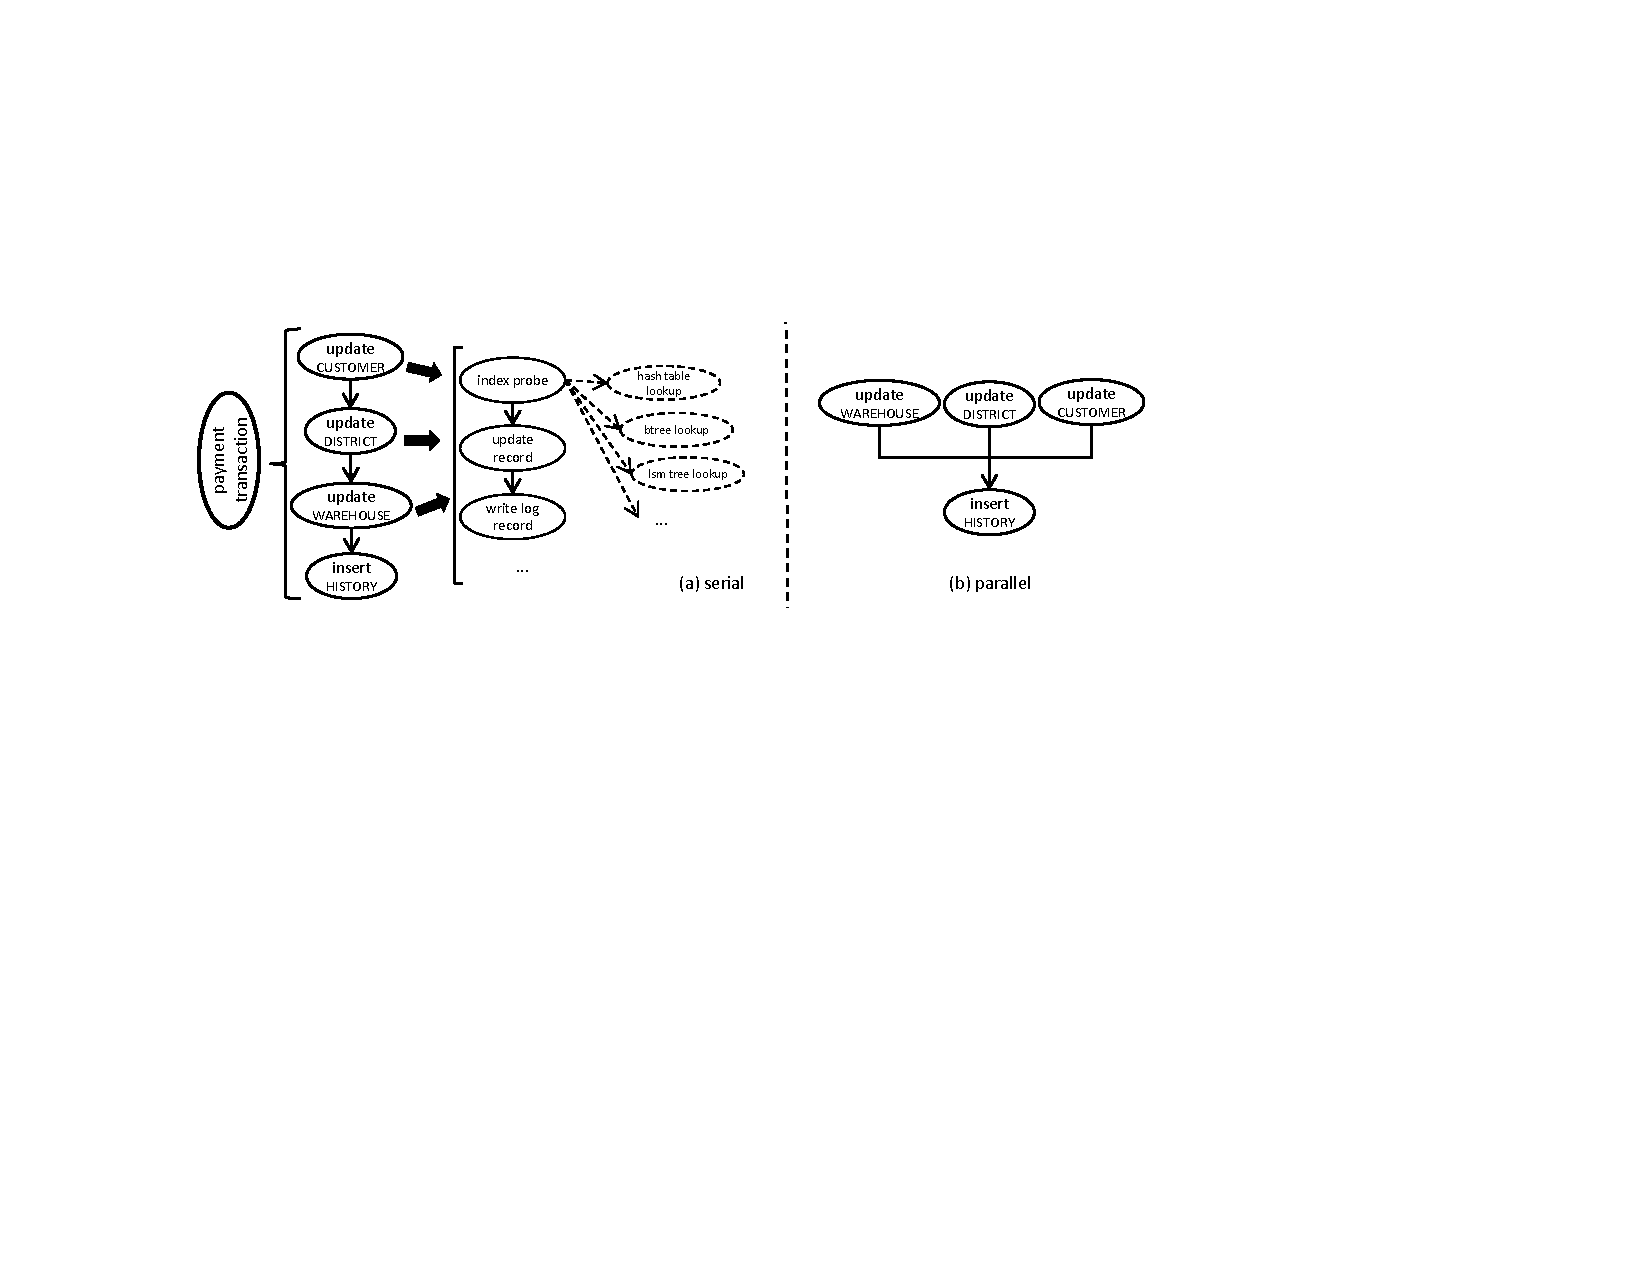
\includegraphics{fig-intrataskgran.pdf}
\caption{TPC-C's \texttt{payment} transaction.
Each node represents a sub-task in \texttt{payment}.
\texttt{Customer}, \texttt{District}, \texttt{Warehouse}, and \texttt{History} are the tables in TPC-C.
(For brevity the iteration over the \texttt{Customer} table in this transaction is omitted).
(a) The serial execution plan also illustrating the sub-tasks of \texttt{payment} at different granularities.
\texttt{payment} performs operations such as update and insert.
An update performs actions such as index probe, update record, write log, etc.
These actions also have sub-tasks at a finer-granularity.
(b) The parallel execution plan for \texttt{payment}
exploiting intra-transaction parallelism among the three independent updates.}
\label{fig:intratask}
\end{figure}

\section{Toward Heterogeneous Parallelism}
\label{sec:het}

As mentioned in \refsec{intro},
adding more and more cores to a processor cannot be the only path for progressing commodity servers anymore.
Moore's Law is slowing down.
The main reason is once again power-related even though there are other physical constraints as well
(e.g., fabrication costs for transistors that get smaller and smaller).
The supply voltage required to power all the transistors up does not decrease at a proportional rate.
Even if we can still add more and more cores on processors,
we will not be able to power all of them up simultaneously \cite{EsmaeilzadehBASB11}.
Optimizing energy per instruction has to be the key in this new era.

One option to achieve more energy-efficient hardware is to adopt simpler and more low-power cores in emerging processors.
However, such processing units are not suitable for latency critical applications.
In addition, solely focusing on the energy-efficiency of an individual core or processor
is not going to give us energy-proportionality \cite{BarrosoH07}.
We have to focus on how much energy it takes to run tasks to completion.
The low-power cores might end up spending more energy at the end of the day for running a set of tasks 
compared to power-hungry cores since it takes them longer to execute tasks due to being slower \cite{LangPS10}.

The better long-term solution for energy-efficiency is to build servers with a variety of processing units,
where each unit is specialized to accelerate specific tasks.
On such servers, one would pick the cores to power-up based on the tasks currently running,
while shutting down the idle cores that are specialized for other types of tasks.
Orchestrating task scheduling dynamically over such heterogeneous hardware intensifies
an already challenging problem on homogeneous hardware (as \refsec{sched} focused on).
In addition, economic feasibility of specialized hardware is always a concern
since specialization limits the market of a system, despite being more efficient,
as opposed to being general-purpose.
%
As a result, processor specialization for data-intensive tasks was unpopular in industry up until recently.
However, this attitude has been changing \cite{AlonsoB18, HennessyP19}. %\cite{catapult, tpu}.
%First, the growing size of data and complexity of data-intensive applications require more and more processing power.
%The slowdown of the evolution of today’s commodity multicore servers require departing from conventional thinking. 
%Second, the increasing scale of the data-intensive applications has started to diminish the economic concerns over specialized hardware.
%Third, the tools that enable more uniform programming interfaces over heterogeneous hardware have been maturing.
%Fourth, major server hardware vendors have been designing products with different types of processing units targeting data-intensive applications.
Therefore, there is pressing need to develop scheduling mechanisms that not only consider
the diversity of the data-intensive tasks, but also the diversity of the processing units.

The scheduling approaches surveyed in \refsec{sched} are inspiring and preliminary steps
toward the efficient utilization of processors with many diverse parallelism opportunities.
The common denominators (and the common root of the associated challenges)
across all of these mechanisms are that
(1) they view data-intensive tasks at a finer sub-task granularity
(e.g., \textit{update} operation of \textit{payment} transaction instead of the whole \textit{payment} transaction)
and (2) they adopt lighter-weight and hardware-topology-aware techniques for dynamic scheduling of these sub-tasks
instead of relying on the traditional operating system defaults.

Splitting data-intensive tasks into their sub-tasks
(see examples in \reffig{common} and \reffig{intratask})
help in identifying the common sub-tasks across concurrent transactions or analytical queries.
This, in turn, enables more opportunities for constructive instruction and data sharing,
intra-task parallelism, and mapping a unit work to a core that would benefit the most from running on that core.
Furthermore, it is an essential preliminary step to 
discover the frequent critical sub-tasks that justify building new specialized hardware for.
Therefore,
even though detecting the right granularity for sub-tasks and orchestrating more things at runtime is a big challenge,
this challenge is worthwhile to address and study in more depth.
It is the only way to answer the \textit{what} question and aides answering the \textit{where} question
in the context of emerging heterogeneous hardware landscape.

After mapping a certain granularity of sub-tasks to the available processing units at runtime,
one has to perform the actual scheduling and coordination of these sub-tasks efficiently.
Otherwise, no matter how optimal the mapping is, it is not going to be beneficial.
Specializing context switching or thread migrations for data-intensive tasks
either at the level of the kernel or hardware has been tried (as also mentioned in \refsec{sched:impl}).
These techniques and others that specialize the same routines
should be revisited in more detail in the context of heterogeneous hardware.
It is highly likely that the common operating system layers and mechanisms will also evolve with such hardware.
Therefore, it is important to have a holistic view while developing mechanisms to efficiently coordinate sub-tasks
in order to achieve lightweight coordination and minimize replication of functionality across layers.
In addition, exploiting more and more processing units should not turn the development
of a data-intensive application into an unproductive process.
Ensuring the correct and efficient instruction and data stream on a specific processing unit should be handled through
high-level language primitives for the application developer and smart query compilation within the data management system
\cite{HeimelSPMM13}.
%\cite{HeimelSPMM13, PirkMZM16}.
Tackling these two challenges is the way to answer the \textit{how} question for heterogeneous many cores.

Next, we discuss an end-to-end framework that takes the challenges of scheduling varying data-intensive tasks
on heterogeneous hardware into account by mainly focusing on the resource estimation challenge,
which also aides the \textit{where} question.

\section{A Framework for Running Data-Intensive Tasks on Emerging Hardware}
\label{sec:guide}

Even though the previous sections focus on the utilization of a single server hardware,
resource-aware scheduling is an active field of research often tailored specifically for different hardware platforms,
from small embedded systems~\cite{Tillenius_2015} up to clusters~\cite{Delimitrou_2014}.
Executing tasks with varying resource demands in parallel can lead to inefficient resource utilization,
especially on heterogeneous hardware.
More precisely, the correlation between the resource demand of a task and its completion time is often highly non-linear,
once the task is executed concurrently with other ones.
In order to solve the very challenging problem of finding an optimal resource mapping for a single task,
new resource-aware scheduling strategies are required,
which efficiently map tasks to heterogeneous parallel architectures,
taking their particular resource demands into account. 
Independent of the actual objective,
i.e., making the execution of hybrid tasks more efficient or
designing an efficient parallelization strategy for a specific task,
the underlying motivation remains the same, namely,
optimizing the execution of tasks on heterogeneous hardware architectures while respecting given latency requirements.

In data management systems,
hybrid data-intensive tasks often arrive dynamically
providing only inaccurate information about their resource utilization behavior.
Unlike classical scheduling problems, such systems require mapping methods that
(1) interact with a resource model to map tasks to suitable resources at runtime and
(2) adjust mapping decisions dynamically depending on the system load. 

Many existing work that tackle the problem of scheduling tasks on parallel architectures
aim to optimize either the execution of tasks having similar characteristics (e.g., only transactional workloads) or
the scheduling of tasks with hybrid characteristics (transactional and analytical workloads) on homogeneous parallel systems.
For example, database systems such as SAP HANA or HyPer are designed to efficiently execute hybrid tasks
using an optimized workload management system for servers with homogeneous cores~\cite{Psaroudakis_2015}.
Future scheduling strategies, however, should consider both the heterogeneity of workloads and of hardware
in order to find an efficient resource-aware mapping exploiting the full potential of the underlying parallel architecture.

To enable a resource-efficient scheduling of data-intensive tasks over complex heterogeneous hardware architectures,
we focus on a framework, illustrated in \reffig{framework},
that includes scheduling mechanisms guided by resource estimation models.
Regarding different aspects of our strategy,
we survey previous approaches harvesting already existing results that shall serve as a guideline.

To generate resource estimation models distinct machine learning methods or analytical models
can be applied to predict the resource demands for different possible task-to-core(s) mapping strategies.
Analytical models can be more accurate than machine learning models
when applied to estimate the runtime of concurrently executed tasks~\cite{Wu_2013}.
However,
machine learning models are typically preferred in more complex heterogeneous hardware scenarios,
since the complexity of the analytical models can increase rapidly in such cases. 
When building models that are capable of describing the complete data management system behavior,
several aspects need to be taken into consideration.
For models with high multidimensionality and thus high complexity,
a dimensionality reduction, through machine learning techniques such as clustering or classification,
is suggested~\cite{Chen_2011}.
For example, as shown by previous work \cite{Ma_2018},
a workload forecasting strategy based on machine learning techniques can try to predict
the expected arrival rate of certain types of tasks in a data management system
and use clustering to reduce the model complexity.
In general, machine learning methods, especially for resource estimations,
are not only applicable to data management systems running on a single server.
They can also be applied in the context of cluster management,
e.g., to classify heterogeneous workloads that would achieve an efficient resource utilization~\cite{Delimitrou_2014}.

\begin{figure}
	\centering
	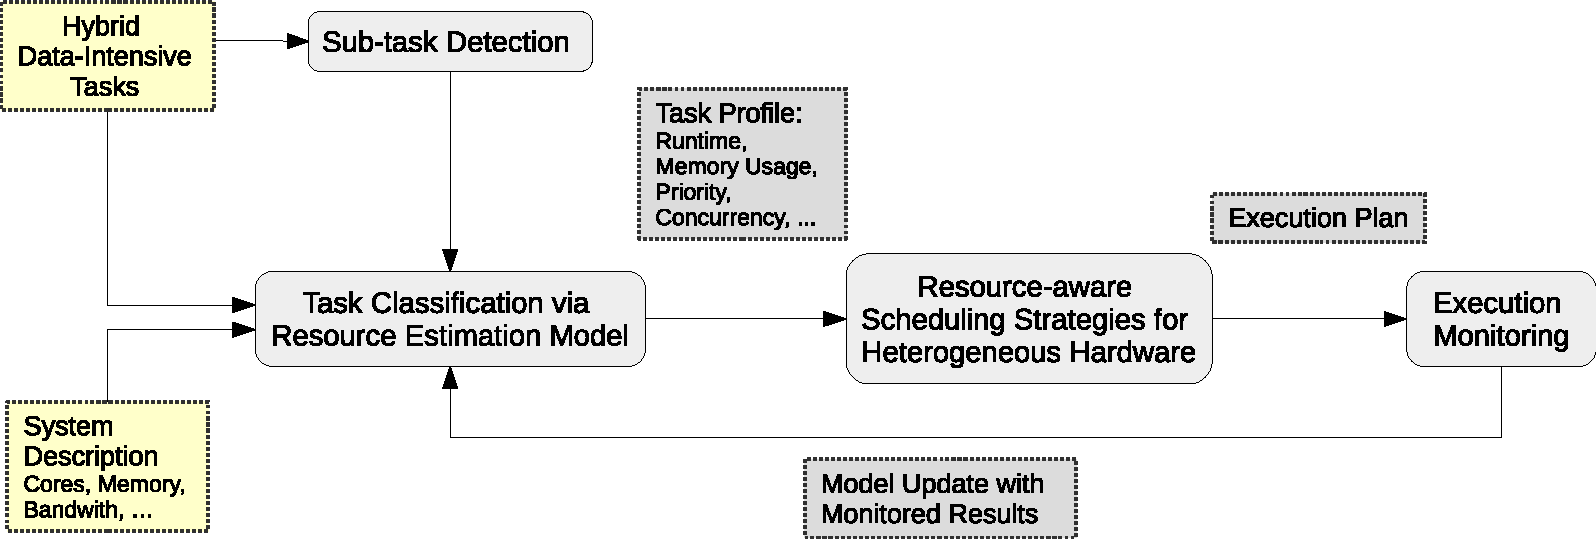
\includegraphics[width=0.95\textwidth]{fig-framework.pdf}
	\caption{Framework for resource-aware scheduling strategies guided by a resource estimation model for hybrid data-intensive tasks executed on heterogeneous hardware.}
	\label{fig:framework}
\end{figure}

\reffig{framework} visualizes the optimization cycle of the resource-aware scheduling framework.
It consists of four main steps.

In the \textit{first} step,
the sub-task detection tries to identify possible sub-tasks from the incoming data-intensive tasks
(transactional and different types of analytical) to take possible parallelization strategies into account.

To determine an efficient mapping of tasks to available hardware,
it is necessary to be aware of each task’s (estimated) resource demand.
To this effect, a flexible resource estimation model is constructed in the \textit{second} step,
which estimates the resource demands of each task and sub-task based on previously executed similar tasks.
Since the available hardware architecture influences the runtime behavior of a task,
the model also uses the hardware description as input,
and later should also be able to adapt to hardware changes.
As mentioned above,
such a model can utilize machine learning techniques instead of analytical cost models,
since the analytical models could become very complex
when they have to cope with many different heterogeneous hardware parts in one system.
Depending on the model's estimations,
tasks can be classified into different types of groups based on their resource demands
to later efficiently map them to suitable hardware resources or queues that are assigned to each group.
Therefore, as an output the model produces task profiles
including different resource utilization characteristics and
an execution priority that can be used for latency critical tasks. 
A similar framework for resource-aware scheduling that focuses on scheduling
parallel parameter optimization of machine learning algorithms with heterogeneous tasks
have been studied in \cite{kotthaus_2017a}.
This framework uses a regression model to estimate the runtime of tasks
and computes an execution priority for each task.
This priority is then used as input to schedule these tasks
in a way that minimizes CPU idling on homogeneous clusters.
Further work on this framework showed that its runtime estimation mechanism also works for heterogeneous hardware.
However, for heterogeneous hardware the random forest regression model is found to be more effective since
task execution times form a discontinuous model
because of the additional categorical variable that represents the processor type~\cite{kotthaus_2018}. 
Besides runtime estimation,
the estimation of multiple performance metrics via machine learning techniques
for specific query plans on homogeneous hardware is proposed in~\cite{Ganapathi_2009}.
In~\cite{Mozafari_2013} a detailed overview of different machine learning techniques applicable for estimating multiple metrics for highly concurrent OLTP workloads on homogeneous systems is given, which could be interesting as well for resource estimations on heterogeneous systems. 

As depicted in \reffig{framework},
the obtained task profiles including multiple metrics serve as inputs for the resource-aware scheduling strategies
in the \textit{third} step.
Resulting from this, an execution plan is created that efficiently maps tasks to suitable hardware resources.
While creating the execution plan, this step also determines whether to use intra-task parallelism or
the degree of parallelism for a task based on the available hardware resources and topology.
As mentioned in \refsec{sched:expl}, due to sub-task coordination efforts and non-uniform core-to-core communication costs,
parallel execution plan of a task may not always result in faster execution compared to running a task serially.

Since the profiles are only estimated, under- or overestimation (e.g., of execution times) may occur.
In such cases, a task may need to be rescheduled or stopped to guarantee latency requirements.
This service is performed by the execution monitoring provided by the \textit{last} step of our strategy.
Here, an adaptive operator replacement technique using machine learning for runtime estimation,
as presented in~\cite{Bress_2014},
could be applied, where operator mappings are dynamically adjusted on heterogeneous co-processors.
Moreover, execution monitoring is also used to gather information about the system behavior, such as CPU or memory utilization, and to measure the de facto resource utilization of tasks at runtime. After a task or a group of tasks has finished their execution, the results are collected to iteratively refine the resource estimation model. Evidently, the quality of the scheduling strategy depends on the accuracy of the resource estimation. Hence, the model update entails more reliable estimations over time for the future predictions of the new incoming tasks.

\section{Conclusion}
\label{sec:conc}

In this article,
we focused on scheduling data-intensive applications with different types of tasks
over the processing units of emerging heterogeneous server hardware.
%targeting the resource utilization of such hardware.
Existing scheduling proposals that diverge from conventional methods when utilizing the resources
of a single server with homogeneous multicores already give us essential insights.
Therefore, their challenges should be revisited in the context of emerging heterogeneous hardware.
More specifically, moving forward we should focus on the following:
(1) identifying sub-tasks of data-intensive tasks across different applications,
especially the common ones that allow constructive sharing of instructions and data,
(2) efficient orchestration of these sub-tasks at runtime,
(3) dynamic models to guide us during task-to-core(s) mapping decisions, and
(4) a holistic approach across hardware, operating systems, and data management/processing systems
to keep the systems' layers lightweight.
This article navigated these items giving a high-level overview.
Our goal is to tackle them in more detail in the future.

%% OLD
%We surveyed existing scheduling proposals that diverge from conventional methods
%when utilizing the resources of a single server with homogeneous multicores and different dimensions of parallelism.
%We identified and followed the three critical questions that any scheduling mechanism must answer
%as we discussed the proposals.
%We consider the insights from these proposals to be essential when targeting heterogeneous platforms as well.
%Therefore, their challenges should be revisited in the context of emerging hardware.
%Furthermore,
%we discussed a resource-aware scheduling framework for hybrid data-intensive tasks running on a heterogeneous server
%emphasizing the importance of resource estimation models in such frameworks.
%Even though we mainly focus on the resource utilization of a single commodity server platform
%while running data-intensive tasks in this article,
%there are common challenges across more resource-constrained environments or large-scale clusters
%as well as other complex applications.

\section*{Acknowledgments}
This work was partly supported by Deutsche Forschungsgemeinschaft (DFG) 
within the Collaborative Research Center SFB 876, projects C5 and A3.
The authors would like to thank Jens Teubner, Philippe Bonnet, and Danica Porobic for providing valuable feedback.

%% 
\begin{thebibliography}{10}
\begin{small}
\itemsep=1pt
%\bibliographystyle{abbrv}
%\bibliography{PTdebullMarch}
\bibitem{AilamakiLTPP17}
A.~Ailamaki, E.~Liarou, P.~T\"oz\"un, D.~Porobic, and I.~Psaroudakis.
\newblock {\em {Databases on Modern Hardware: How to Stop Underutilization and
  Love Multicores}}.
\newblock Morgan {\&} Claypool Publishers, 2017.

\bibitem{AlonsoB18}
G.~Alonso and P.~Bailis.
\newblock {Research for practice: FPGAs in datacenters}.
\newblock {\em {CACM}}, 61(9):48--49, 2018.

\bibitem{AttaTAM12-2}
I.~Atta, P.~T\"oz\"un, A.~Ailamaki, and A.~Moshovos.
\newblock {SLICC}: {S}elf-{A}ssembly of {I}nstruction {C}ache {C}ollectives for
  {OLTP} {W}orkloads.
\newblock In {\em MICRO}, pages 188--198, 2012.

\bibitem{AttaTTAM13}
I.~Atta, P.~T\"oz\"un, X.~Tong, A.~Ailamaki, and A.~Moshovos.
\newblock {STREX}: {B}oosting {I}nstruction {C}ache {R}euse in {OLTP}
  {W}orkloads through {S}tratified {T}ransaction {E}xecution.
\newblock In {\em ISCA}, pages 273--284, 2013.

\bibitem{BarrosoH07}
L.~A. Barroso and U.~H\"{o}lzle.
\newblock {The Case for Energy-Proportional Computing}.
\newblock {\em Computer}, 40:33--37, 2007.

\bibitem{Bress_2014}
S.~Bre\ss, B.~K\"{o}cher, M.~Heimel, V.~Markl, M.~Saecker, and G.~Saake.
\newblock {Ocelot/HyPE: Optimized Data Processing on Heterogeneous Hardware}.
\newblock {\em PVLDB}, 7(13):1609--1612, 2014.

\bibitem{ChakrabortyWS06}
K.~Chakraborty, P.~M. Wells, and G.~S. Sohi.
\newblock Computation {S}preading: {E}mploying {H}ardware {M}igration to
  {S}pecialize {CMP} {C}ores {O}n-the-{F}ly.
\newblock In {\em ASPLOS}, pages 283--292, 2006.

\bibitem{Chen_2011}
Y.~Chen, A.~Ganapathi, and R.~Katz.
\newblock {Challenges and Opportunities for Managing Data Systems Using
  Statistical Models}.
\newblock In {\em IEEE DeBull}, volume~34, pages 53--60, 2011.

\bibitem{Delimitrou_2014}
C.~Delimitrou and C.~Kozyrakis.
\newblock {Quasar: Resource-efficient and QoS-aware Cluster Management}.
\newblock In {\em ASPLOS}, pages 127--144, 2014.

\bibitem{DennardGYRBAL74}
R.~H. Dennard, F.~H. Gaensslen, H.-N. Yu, V.~L. Rideout, E.~Bassous, Andre, and
  R.~Leblanc.
\newblock Design of {I}on-{I}mplanted {MOSFET}s with {V}ery {S}mall {P}hysical
  {D}imensions.
\newblock {\em IEEE J. Solid-State Circuits}, pages 256--268, 1974.

\bibitem{EsmaeilzadehBASB11}
H.~Esmaeilzadeh, E.~Blem, R.~St.~Amant, K.~Sankaralingam, and D.~Burger.
\newblock Dark {S}ilicon and the {E}nd of {M}ulticore {S}caling.
\newblock In {\em ISCA}, pages 365--376, 2011.

\bibitem{Ferdman+12}
M.~Ferdman, A.~Adileh, O.~Kocberber, S.~Volos, M.~Alisafaee, D.~Jevdjic,
  C.~Kaynak, A.~D. Popescu, A.~Ailamaki, and B.~Falsafi.
\newblock Clearing the {C}louds: {A} {S}tudy of {E}merging {S}cale-out
  {W}orkloads on {M}odern {H}ardware.
\newblock In {\em ASPLOS}, pages 37--48, 2012.

\bibitem{Ganapathi_2009}
A.~{Ganapathi}, H.~{Kuno}, U.~{Dayal}, J.~L. {Wiener}, A.~{Fox}, M.~{Jordan},
  and D.~{Patterson}.
\newblock {Predicting Multiple Metrics for Queries: Better Decisions Enabled by
  Machine Learning}.
\newblock In {\em ICDE}, pages 592--603, 2009.

\bibitem{GiannikisAK12}
G.~Giannikis, G.~Alonso, and D.~Kossmann.
\newblock {SharedDB: Killing One Thousand Queries With One Stone}.
\newblock {\em {PVLDB}}, 5(6):526--537, 2012.

\bibitem{GicevaZAR16}
J.~Giceva, G.~Zellweger, G.~Alonso, and T.~Roscoe.
\newblock {Customized OS support for data-processing}.
\newblock In {\em DaMoN}, pages 2:1--2:6, 2016.

\bibitem{Hamilton10}
J.~Hamilton.
\newblock {Perspectives - Overall Data Center Costs}.
\newblock
  \url{https://perspectives.mvdirona.com/2010/09/overall-data-center-costs/}.

\bibitem{HarizopoulosA04}
S.~Harizopoulos and A.~Ailamaki.
\newblock {STEPS} {T}owards {C}ache-{R}esident {T}ransaction {P}rocessing.
\newblock In {\em VLDB}, pages 660--671, 2004.

\bibitem{HarizopoulosSA05}
S.~Harizopoulos, V.~Shkapenyuk, and A.~Ailamaki.
\newblock {QP}ipe: {A} {S}imultaneously {P}ipelined {R}elational {Q}uery
  {E}ngine.
\newblock In {\em SIGMOD}, pages 383--394, 2005.

\bibitem{HeimelSPMM13}
M.~Heimel, M.~Saecker, H.~Pirk, S.~Manegold, and V.~Markl.
\newblock {Hardware-Oblivious Parallelism for In-Memory Column-Stores}.
\newblock {\em {PVLDB}}, 6(9):709--720, 2013.

\bibitem{HennessyP19}
J.~L. Hennessy and D.~A. Patterson.
\newblock {A new golden age for computer architecture}.
\newblock {\em {CACM}}, 62(2):48--60, 2019.

\bibitem{kotthaus_2018}
H.~Kotthaus.
\newblock {\em {Methods for Efficient Resource Utilization in Statistical
  Machine Learning Algorithms}}.
\newblock PhD thesis, TU Dortmund University, 2018.

\bibitem{kotthaus_2017a}
H.~Kotthaus, J.~Richter, A.~Lang, J.~Thomas, B.~Bischl, P.~Marwedel,
  J.~Rahnenführer, and M.~Lang.
\newblock {RAMBO: Resource-Aware Model-Based Optimization with Scheduling for
  Heterogeneous Runtimes and a Comparison with Asynchronous Model-Based
  Optimization}.
\newblock In {\em LION}, pages 180--195, 2017.

\bibitem{LangPS10}
W.~Lang, J.~M. Patel, and S.~Shankar.
\newblock Wimpy {N}ode {C}lusters: {W}hat {A}bout {N}on-{W}impy {W}orkloads?
\newblock In {\em DaMoN}, pages 47--55, 2010.

\bibitem{LarusP02}
J.~R. Larus and M.~Parkes.
\newblock {Using Cohort-Scheduling to Enhance Server Performance}.
\newblock In {\em USENIX}, pages 103--114, 2002.

\bibitem{LeisBKN14}
V.~Leis, P.~A. Boncz, A.~Kemper, and T.~Neumann.
\newblock {Morsel-driven parallelism: a NUMA-aware query evaluation framework
  for the many-core age}.
\newblock In {\em SIGMOD}, pages 743--754, 2014.

\bibitem{Ma_2018}
L.~Ma, D.~Van~Aken, A.~Hefny, G.~Mezerhane, A.~Pavlo, and G.~J. Gordon.
\newblock {Query-based Workload Forecasting for Self-Driving Database
  Management Systems}.
\newblock In {\em SIGMOD}, pages 631--645, 2018.

\bibitem{Moore65}
G.~Moore.
\newblock Cramming {M}ore {C}omponents onto {I}ntegrated {C}ircuits.
\newblock {\em Electronics}, 38(6), 1965.

\bibitem{Mozafari_2013}
B.~Mozafari, C.~Curino, A.~Jindal, and S.~Madden.
\newblock {Performance and Resource Modeling in Highly-concurrent OLTP
  Workloads}.
\newblock In {\em SIGMOD}, pages 301--312, 2013.

\bibitem{OlukotunNHWC96}
K.~Olukotun, B.~A. Nayfeh, L.~Hammond, K.~Wilson, and K.~Chang.
\newblock The {C}ase for a {S}ingle-{C}hip {M}ultiprocessor.
\newblock In {\em ASPLOS}, pages 2--11, 1996.

\bibitem{OzcanTT17}
F.~{\"{O}}zcan, Y.~Tian, and P.~T{\"{o}}z{\"{u}}n.
\newblock {Hybrid Transactional/Analytical Processing: A Survey}.
\newblock In {\em SIGMOD}, pages 1771--1775, 2017.

\bibitem{Pandis+11}
I.~Pandis, P.~T\"oz\"un, M.~Branco, D.~Karampinas, D.~Porobic, R.~Johnson, and
  A.~Ailamaki.
\newblock A {D}ata-{O}riented {T}ransaction {E}xecution {E}ngine and
  {S}upporting {T}ools.
\newblock In {\em SIGMOD}, pages 1237--1240, 2011.

\bibitem{PandisTJA11}
I.~Pandis, P.~T\"oz\"un, R.~Johnson, and A.~Ailamaki.
\newblock {PLP}: {P}age {L}atch-{F}ree {S}hared-{E}verything {OLTP}.
\newblock {\em PVLDB}, 4(10):610--621, 2011.

\bibitem{PorobicLTA14}
D.~Porobic, E.~Liarou, P.~T\"oz\"un, and A.~Ailamaki.
\newblock {ATraPos:} {A}daptive {T}ransaction {P}rocessing on {H}ardware
  {I}slands.
\newblock In {\em ICDE}, pages 688--699, 2014.

\bibitem{PsaroudakisAA13}
I.~Psaroudakis, M.~Athanassoulis, and A.~Ailamaki.
\newblock {S}haring {D}ata and {W}ork {A}cross {C}oncurrent {A}nalytical
  {Q}ueries.
\newblock {\em PVLDB}, 6(9):637--648, 2013.

\bibitem{PsaroudakisSMSA15}
I.~Psaroudakis, T.~Scheuer, N.~May, A.~Sellami, and A.~Ailamaki.
\newblock {Scaling Up Concurrent Main-Memory Column-Store Scans: Towards
  Adaptive NUMA-aware Data and Task Placement}.
\newblock {\em {PVLDB}}, 8:1442--1453, 2015.

\bibitem{Psaroudakis_2015}
I.~Psaroudakis, F.~Wolf, N.~May, T.~Neumann, A.~B{\"o}hm, A.~Ailamaki, and
  K.-U. Sattler.
\newblock {Scaling Up Mixed Workloads: A Battle of Data Freshness, Flexibility,
  and Scheduling}.
\newblock In {\em TPCTC}, pages 97--112, 2014.

\bibitem{SirinTPA16}
U.~Sirin, P.~T{\"{o}}z{\"{u}}n, D.~Porobic, and A.~Ailamaki.
\newblock {Micro-architectural Analysis of In-memory OLTP}.
\newblock In {\em SIGMOD}, pages 387--402, 2016.

\bibitem{Tillenius_2015}
M.~Tillenius, E.~Larsson, R.~M. Badia, and X.~Martorell.
\newblock {Resource-Aware Task Scheduling}.
\newblock {\em ACM TECS}, 14(1):5:1--5:25, 2015.

\bibitem{TozunAAM14}
P.~T\"oz\"un, I.~Atta, A.~Ailamaki, and A.~Moshovos.
\newblock {ADDICT}: {A}dvanced {I}nstruction {C}hasing for {T}ransactions.
\newblock {\em PVLDB}, 7(14):1893--1904, 2014.

\bibitem{TPCC}
{TPC} {B}enchmark {C} {S}tandard {S}pecification.
\newblock \url{http://www.tpc.org/tpcc}.

\bibitem{Wu_2013}
W.~Wu, Y.~Chi, H.~Hac\'{\i}g\"{u}m\"{u}\c{s}, and J.~F. Naughton.
\newblock {Towards Predicting Query Execution Time for Concurrent and Dynamic
  Database Workloads}.
\newblock {\em PVLDB}, 6(10):925--936, 2013.

\bibitem{ZhouCRS05}
J.~Zhou, J.~Cieslewicz, K.~A. Ross, and M.~Shah.
\newblock {Improving Database Performance on Simultaneous Multithreading
  Processors}.
\newblock In {\em VLDB}, pages 49--60, 2005.
\end{small}
\end{thebibliography} 

\end{document}

\end{article}

\begin{article}
{Optimistic Lock Coupling: A Scalable and Efficient General-Purpose Synchronization Method}
{Viktor Leis, Michael Haubenschild, Thomas Neumann}
\graphicspath{{submissions/vleis/figs/}}
\pdfminorversion=5
\documentclass[11pt]{article}
\usepackage{deauthor,times,graphicx,caption,microtype}
\usepackage{hyperref}
\usepackage{listings}
\usepackage{booktabs}

\begin{document}

\title{Optimistic Lock Coupling: A Scalable and Efficient General-Purpose Synchronization Method}

\author{Viktor Leis, Michael Haubenschild\raisebox{0.9ex}{$\ast$}, Thomas Neumann\\ Technische Universit{\"a}t M{\"u}nchen \hspace{0.7cm} Tableau Software\raisebox{0.9ex}{$\ast$} \\ {\{leis,neumann\}{@}in.tum.de} \hspace{0.7cm} {mhaubenschild{@}tableau.com\raisebox{0.9ex}{$\ast$}}}

\maketitle

\begin{abstract}
As the number of cores on commodity processors continues to increase, scalability becomes more and more crucial for overall performance.
Scalable and efficient concurrent data structures are particularly important, as these are often the building blocks of parallel algorithms.
Unfortunately, traditional synchronization techniques based on fine-grained locking have been shown to be unscalable on modern multi-core CPUs.
Lock-free data structures, on the other hand, are extremely difficult to design and often incur significant overhead.

In this work, we make the case for Optimistic Lock Coupling as a practical alternative to both traditional locking and the lock-free approach.
We show that Optimistic Lock Coupling is highly scalable and almost as simple to implement as traditional lock coupling.
Another important advantage is that it is easily applicable to most tree-like data structures.
We therefore argue that Optimistic Lock Coupling, rather than a complex and error-prone custom synchronization protocol, should be the default choice for performance-critical data structures.
\end{abstract}

\section{Introduction}

% more and more cores
Today, Intel's commodity server processors have up to 28 cores and its upcoming microarchitecture will have up to 48 cores per socket~\cite{intel}.
Similarly, AMD currently stands at 32 cores and this number is expected to double in the next generation~\cite{amd}.
Since both platforms support simultaneous multithreading (also known as hyperthreading), affordable commodity servers (with up to two sockets) will soon routinely have between 100 and 200 hardware threads.

% data structure scalability is important
With such a high degree of hardware parallelism, efficient data processing crucially depends on how well concurrent data structures scale.
Internally, database systems use a plethora of data structures like table heaps, internal work queues, and, most importantly, index structures.
Any of these can easily become a scalability (and therefore overall performance) bottleneck on many-core CPUs.

% traditional synchronization: fine-grained locks, slow, cache invalidation
Traditionally, database systems synchronize internal data structures using fine-grained reader/writer locks\footnote{In this work, we focus on data structure synchronization rather than high-level transaction semantics and therefore use the term {\em lock} for what would typically be called {\em latch} in the database literature. We thus follow common computer science (rather than database) terminology.}.
Unfortunately, while fine-grained locking makes lock contention unlikely, it still results in bad scalability because lock acquisition and release require writing to shared memory.
Due to the way cache coherency is implemented on modern multi-core CPUs, these writes cause additional cache misses\footnote{The cache coherency protocol ensures that all copies of a cache line on other cores are invalidated before the write can proceed.} and the cache line containing the lock's internal data becomes a point of physical contention.
As a result, any frequently-accessed lock (e.g., the lock of the root node of a B-tree) severely limits scalability.

% lock-free bw-tree: no more latches, but indirections, extremely complex
Lock-free data structures like the Bw-tree~\cite{DBLP:conf/icde/LevandoskiLS13a} (a lock-free B-tree variant) or the Split-Ordered List~\cite{DBLP:journals/jacm/ShalevS06} (a lock-free hash table) do not acquire any locks and therefore generally scale much better than locking-based approaches (in particular for read-mostly workloads).
However, lock-free synchronization has other downsides:
First, it is very difficult and results in extremely complex and error-prone code (when compared to locking).
Second, because the functionality of atomic primitives provided by the hardware (e.g., atomically compare-and-swap 8 bytes) is limited, complex operations require additional indirections within the data structure.
For example, the Bw-tree requires an indirection table and the Split-Ordered List requires ``dummy nodes'', resulting in overhead due to additional cache misses.

% OLC for the win
In this paper we make the case for {\em Optimistic Lock Coupling (OLC)}, a synchronization method that combines some of the best properties of lock-based and lock-free synchronization.
OLC utilizes a special lock type that can be used in two modes:
The first mode is similar to a traditional mutex and excludes other threads by physically acquiring the underlying lock.
In the second mode, reads can proceed optimistically by validating a version counter that is embedded in the lock (similar to optimistic concurrency control).
The first mode is typically used by writers and the second mode by readers.
Besides this special lock type, OLC is based on the observation that optimistic lock validations can be interleaved/coupled---similar to the pair-wise interleaved lock acquisition of traditional lock coupling.
Hence, the name Optimistic Lock Coupling.

OLC has a number of desirable features:
\begin{itemize}
\item By reducing the number of writes to shared memory locations and thereby avoiding cache invalidations, it {\bf scales well} for most workloads.
\item In comparison to unsynchronized code, it requires few additional CPU instructions making it {\bf efficient}.
\item OLC is {\bf widely applicable} to different data structures. It has already been successfully used for synchronizing binary search trees~\cite{DBLP:conf/ppopp/BronsonCCO10}, tries~\cite{artsync}, trie/B-tree hybrids~\cite{DBLP:dblp_conf/eurosys/MaoKM12}, and B-trees~\cite{buzzword}.
\item In comparison to the lock-free paradigm, it is also {\bf easy to use} and requires few modifications to existing, single-threaded data structures.
\end{itemize}
Despite these positive features and its simplicity, OLC is not yet widely known.
The goal of this paper is therefore to popularize this simple idea and to make a case for it.
We argue that OLC deserves to be widely known.
It is a good default synchronization paradigm---more complex, data structure-specific protocols are seldom beneficial.

The rest of the paper is organized as follows.
Section~\ref{sec:related} discusses related work, tracing the history of OLC and its underlying ideas in the literature.
The core of the paper is Section~\ref{sec:olc}, which describes the ideas behind OLC and how it can be used to synchronize complex data structures.
In Section~\ref{sec:evaluation} we experimentally show that OLC has low overhead and scales well when used to synchronize an in-memory B-tree.
We summarize the paper in Section~\ref{sec:conc}.

\newpage
\section{Related Work}\label{sec:related}

Lock coupling has been proposed as a method for allowing concurrent operations on B-trees in 1977~\cite{DBLP:journals/acta/BayerS77}.
This traditional and still widely-used method, described in detail in Graefe's B-tree survey~\cite{DBLP:journals/ftdb/Graefe11}, is also called ``latch coupling'', ``hand-over-hand locking'', and ``crabbing''.
Because at most two locks are held at-a-time during tree traversal, this technique seemingly allows for a high degree of parallelism---in particular if read/write locks are used to enable inner nodes to be locked in shared mode.
However, as we show in Section~\ref{sec:evaluation}, on modern hardware lock acquisition (even in shared mode) results in suboptimal scalability.

An early alternative from 1981 is a B-tree variant called B-link tree~\cite{DBLP:journals/tods/LehmanY81}, which only holds a single lock at a time.
It is based on the observation that between the release of the parent lock and the acquisition of the child lock, the only ``dangerous'' thing that could have happened is the split of a child node (assuming one does not implement merge operations).
Thus, when a split happens, the key being searched might end up on a neighboring node to the right of the current child node.
A B-link tree traversal therefore detects this condition and, if needed, transparently proceeds to the neighboring node.
Releasing the parent lock early is highly beneficial when the child node needs to be fetched from disk.
For in-memory workloads, however, the B-link tree has the same scalability issues as lock coupling (it acquires just as many locks).

The next major advance, Optimistic Latch-Free Index Traversal (OLFIT)~\cite{DBLP:conf/vldb/ChaHKK01}, was proposed in 2001.
OLFIT introduced the idea of a combined lock/update counter, which we call {\em optimistic lock}. % , for lack of a better name,
Based on these per-node optimistic locks and the synchronization protocol of the B-link tree, OLFIT finally achieves good scalability on parallel processors.
The OLFIT protocol is fairly complex, as it requires both the non-trivial B-link protocol and optimistic locks.
Furthermore, like the B-link tree protocol, it does not support merging nodes, and is specific to B-trees (cannot easily be applied to other data structures).

In the following two decades, the growth of main-memory capacity led to much research into other data structures besides the venerable B-tree.
Particularly relevant for our discussion is Bronson et al.'s~\cite{DBLP:conf/ppopp/BronsonCCO10} concurrent binary search tree, which is based on optimistic version validation and has a sophisticated, data structure-specific synchronization protocol.
To the best of our knowledge, this 2010 paper is the first that, as part of its protocol, interleaves version validation across nodes---rather than validating each node separately like OLFIT.
In that paper, this idea is called ``hand-over-hand, optimistic validation'', while we prefer the term Optimistic Lock Coupling to highlight the close resemblance to traditional lock coupling.
Similarly, Mao et al.'s~\cite{DBLP:dblp_conf/eurosys/MaoKM12} Masstree (a concurrent hybrid trie/B-tree) is also based on the same ideas, but again uses them as part of a more complex protocol.

The Adaptive Radix Tree (ART)~\cite{art} is another recent in-memory data structure, which we proposed in 2013.
In contrast to the two data structures just mentioned, it was originally designed with single-threaded performance in mind without supporting concurrency.
To add support for concurrency, we initially started designing a custom protocol called Read-Optimized Write Exclusion (ROWEX)~\cite{artsync}, which turned out to be non-trivial and requires modifications of the underlying data structure\footnote{Note that ROWEX is already easier to apply to existing data structures than the lock-free approach. The difficulty depends on the data structure. Applying ROWEX is hard for B-trees with sorted keys and fairly easy for copy-on-write data structures like the Height Optimized Trie~\cite{hot}---with ART being somewhere in the middle.}.
However, fairly late in the project, we also realized, that OLC {\em alone} (rather than as part of a more complex protocol) is sufficient to synchronize ART.
No other changes to the data structure were necessary.
Both approaches were published and experimentally evaluated in a followup paper~\cite{artsync}, which shows that, despite its simplicity, OLC is efficient, scalable, and generally outperforms ROWEX.

Similar results were recently published regarding B-trees~\cite{buzzword}.
In this experimental study a simple OLC-based synchronization outperformed the Bw-tree~\cite{DBLP:conf/icde/LevandoskiLS13a}, a complex lock-free synchronization approach.
Another recent paper shows that for write-intensive workloads, locking often performs better than lock-free synchronization~\cite{DBLP:conf/cidr/FaleiroA17}.
These experiences indicate that OLC is a general-purpose synchronization paradigm and motivate the current paper.

%foster b-tree\cite{DBLP:journals/tods/GraefeKK12}
%Shasha theory~\cite{DBLP:journals/tods/ShashaG88}

\section{Optimistic Lock Coupling}\label{sec:olc}

% locks suck
The standard technique for inter-thread synchronization is mutual exclusion using fine-grained locks.
In a B-tree, for example, every node usually has its own associated lock, which is acquired before accessing that node.
The problem of locking on modern multi- and many-core processors is that lock acquisition and release require writing to the shared memory location that implements the lock.
This write causes exclusive ownership of the underlying cache line and invalidates copies of it on all other processor cores.
For hierarchical, tree-like data structures, the lock of the root node becomes a point of physical contention---even in read-only workloads and even when read/write locks are used.
Depending on the specific data structure, number of cores, cache coherency protocol implementation, cache topology, whether Non-Uniform Memory Access (NUMA) is used, locking can even result in multi-threaded performance that is worse than single-threaded execution.

% in b-trees this happens very much
The inherent pessimism of locking is particularly unfortunate for B-trees:
Despite the fact that logical modifications of the root node are very infrequent, every B-tree operation must lock the root node during tree traversal\footnote{To a lesser extent this obviously applies to all inner nodes, not just the root.}.
Even the vast majority of update operations (with the exception of splits and merges), only modify a single leaf node.
These observations indicate that a more optimistic approach, which does not require locking inner nodes, would be very beneficial for B-trees.

\subsection{Optimistic Locks}

% optimism to the rescue
As the name indicates, optimistic locks try to solve the scalability issues of traditional locks using an optimistic approach.
Instead of always physically acquiring locks, even for nodes that are unlikely to be modified simultaneously, after-the-fact validation is used to detect conflicts.
This is done by augmenting each lock with a version/update counter that is incremented on every modification.
Using this version counter, readers can optimistically proceed before validating that the version did not change to ensure that the read was safe.
If validation fails, the operation is restarted.

% details on opt locks
Using optimistic locks, a read-only node access (i.e., the majority of all operations in a B-tree) does not acquire the lock and does not increment the version counter.
Instead, it performs the following steps:
\begin{enumerate}
\item read lock version (restart if lock is not free)
\item access node
\item read the version again and validate that it has not changed in the meantime
\end{enumerate}
If the last step (the validation) fails, the operation has to be restarted.
Write operations, on the other hand, are more similar to traditional locking:
\begin{enumerate}
\item acquire lock (wait if necessary)
\item access/write to node
\item increment version and unlock node
\end{enumerate}
Writes can therefore protect a node from other writes.

% similar to locks
As we observed in an earlier paper~\cite{artsync}, because of similar semantics, optimistic locks can be hidden behind an API very similar to traditional read/write locks.
Both approaches have an exclusive lock mode, and acquiring a traditional lock in shared mode is analogous to optimistic version validation.
Furthermore, like with some implementations of traditional read/write locks, optimistic locks allow upgrading a shared lock to an exclusive lock.
Lock upgrades are, for example, used to avoid most B-tree update operations from having to lock inner nodes.
In our experience, the close resemblance of optimistic and traditional locks simplifies the reasoning about optimistic locks;
one can apply similar thinking as in traditional lock-based protocols.

\subsection{Lock Coupling with Optimistic Locks}

\begin{figure}
  \centering
  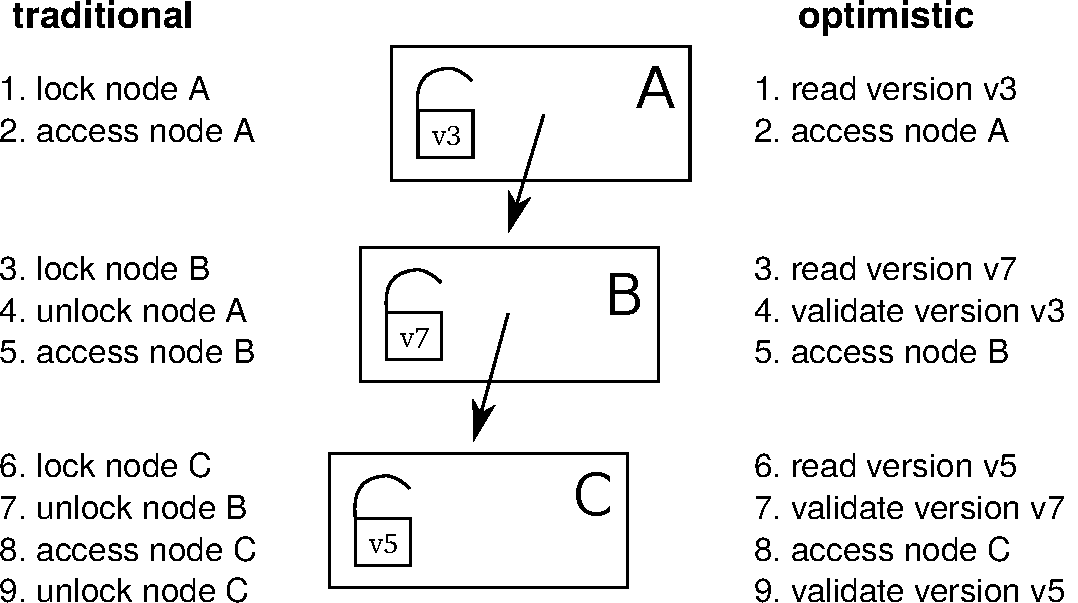
\includegraphics[width=0.65\linewidth]{olcall.pdf}
  \vspace{0.2cm}
  \caption{Comparison of a lookup operation in a 3-level tree using traditional lock coupling (left-hand side) vs.~optimistic lock coupling (right-hand side).}
  \label{fig:olc}
\end{figure}

The traditional and most common lock-based synchronization protocol for B-trees is lock coupling, which interleaves lock acquisitions while holding at most two locks at a time.
If, as we observed earlier, optimistic locks have similar semantics as traditional locks, it is natural to ask whether lock coupling can be combined with optimistic locks.
And indeed the answer is yes: One can almost mechanically translate traditional lock coupling code to optimistic lock coupling code.
This is illustrated in Figure~\ref{fig:olc}, which compares the traversal in a tree of height 3 using traditional and optimistic locks.
As the figure shows, the main difference is that locking is translated to reading the version and that unlocking becomes validation of the previously read version.
This simple change provides efficient lock-free tree traversal without the need to design a complex synchronization protocol.

It is important to emphasize the conceptual simplicity of OLC in comparison to data structures that use custom protocols like the Bw-tree~\cite{DBLP:conf/icde/LevandoskiLS13a}.
To implement lock-free access, the Bw-tree requires an indirection table, delta nodes, complex splitting and merging logic, retry logic, etc.
OLC, on the other hand, can directly be applied to B-trees mostly by adding the appropriate optimistic locking code and without modifying the node layout itself.
Therefore, OpenBw-Tree, an open source implementation of the Bw-tree, requires an order of magnitude more code than a B-tree based on OLC\footnote{Both implementations are available on GitHub: \url{https://github.com/wangziqi2016/index-microbench}}.
Given how difficult it is to develop, validate, and debug lock-free code, simplicity is obviously a major advantage.

\subsection{Correctness Aspects}

\begin{figure}
  % \centering
  %[basicstyle=\normalsize\ttfamily,showstringspaces=false,columns=fullflexible,breaklines=false,breakatwhitespace=true,numbers=none,numberstyle=\small,style=C,keepspaces=true]
\begin{lstlisting}[basicstyle=\ttfamily,language=C++,numbers=left,numberstyle=\small]
std::atomic<BTreeNode*> root;

// search for key in B+tree, returns payload in resultOut
bool lookup(Key key, Value& resultOut) {
   BTreeNode* node = root.load();
   uint64_t nodeVersion = node->readLockOrRestart();
   if (node != root.load()) // make sure the root is still the root
      restart();

   BTreeInner<Key>* parent = nullptr;
   uint64_t parentVersion = 0;

   while (node->isInner()) {
      auto inner = (BTreeInner*)node;

      // unlock parent and make current node the parent
      if (parent)
         parent->readUnlockOrRestart(parentVersion);
      parent = inner;
      parentVersion = nodeVersion;

      // search for next node
      node = inner->findChild(key);
      // validate 'inner' to ensure that 'node' pointer is valid
      inner->checkOrRestart(nodeVersion);
      // now it safe to dereference 'node' pointer (read its version)
      nodeVersion = node->readLockOrRestart();
   }

   // search in leaf and retrieve payload
   auto leaf = (BTreeLeaf*)node;
   bool success = leaf->findValue(key, resultOut);

   // unlock everything
   if (parent)
      parent->readUnlockOrRestart(parentVersion);
   node->readUnlockOrRestart(nodeVersion);

   return success;
}
\end{lstlisting}
  \vspace{0.2cm}
  \caption{B-tree lookup code using OLC. For simplicity, the restart logic is not shown.}
  \label{fig:lookup}
\end{figure}

So far, we have introduced the high-level ideas behind OLC and have stressed its similarity to traditional lock coupling.
Let us now discuss some cases where the close similarity between lock coupling and OLC breaks down.
To make this more concrete, we show the B-tree lookup code in Figure~\ref{fig:lookup}.
In the code, \texttt{readLockOrRestart} reads the lock version and \texttt{readUnlockOrRestart} validates that the read was correct.

One issue with OLC is that any pointer speculatively read from a node may point to invalid memory (if that node is modified concurrently).
Dereferencing such a pointer (e.g., to read its optimistic lock), may cause a segmentation fault or undefined behavior.
In the code shown in Figure~\ref{fig:lookup}, this problem is prevented by the extra check in line 25, which ensures that the read from the node containing the pointer was correct.
Without this additional validation, the code would in line 27 dereference the pointer speculatively read in line 23.
Note that the implementation of \texttt{checkOrRestart} is actually identical to \texttt{readUnlockOrRestart}.
We chose to give it a different name to highlight the fact that this extra check would not be necessary with read/write locks.

Another potential issue with optimistic locks is code that does not terminate.
Code that speculatively accesses a node, like an intra-node binary search, should be written in a way such that it always terminates---even in the presence of concurrent writes.
Otherwise, the validation code that detects the concurrent write will never run.
The binary search of a B-tree, for example, needs to be written in such a way that each comparison makes progress.
For some data structures that do not require loops in the traversal code (like ART) termination is trivially true.

\subsection{Implementation Details}

% implementation, efficiency
To implement an optimistic lock, one can combine the lock and the version counter into a single 64-bit\footnote{Even after subtracting one bit for the lock status, a back-of-the-envelope calculation can show that 63 bits are large enough to never overflow in practice.} word~\cite{artsync}.
A typical read operation will therefore merely consist of reading this version counter atomically.
In C++11 this can be implemented using the \texttt{std::atomic} type.

On x86, atomic reads are cheap because of x86's strong memory order guarantees.
No memory fences are required for sequentially-consistent loads, which are translated (by both GCC and clang) into standard \texttt{MOV} instructions.
Hence, the only effect of \texttt{std::atomic} for loads is preventing instruction re-ordering.
This makes version access and validation cheap.
Acquiring and releasing an optimistic lock in exclusive mode has comparable cost to a traditional lock:
A fairly expensive sequentially-consistent store is needed for acquiring a lock, while a standard \texttt{MOV} suffices for releasing it.
A simple sinlock-based implementation of optimistic locks can be found in the appendix of an earlier paper~\cite{artsync}.

OLC code must be able to handle restarts since validation or lock upgrade can fail due to concurrent writers.
Restarts can easily be implemented by wrapping the data structure operation in a loop (for simplicity not shown in Figure~\ref{fig:lookup}).
Such a loop also enables limiting the number of optimistic retry operations and falling back to pessimistic locking in cases of very heavy contention.
The ability to fall back to traditional locking is a major advantage of OLC in terms of robustness over lock-free approaches, which do not have this option.

In addition to the optimistic shared mode and the exclusive mode, optimistic locks also support a ``shared pessimistic'' mode, which physically acquires the lock in shared mode (allowing multiple concurrent readers but no writers).
This mode is useful for table (or range) scans that touch many tuples on a leaf page (which would otherwise easily abort).
Finally, let us mention that large range scans and table scans, should be broken up into several per-node traversals as is done in the LeanStore~\cite{leanstore} system.

Like all lock-free data structures, but unlike traditional locking and Hardware Transactional Memory~\cite{DBLP:conf/hpca/KarnagelDRLLSL14,DBLP:journals/pvldb/MakreshanskiLS15,htmtkde}, OLC requires care when deleting (and reusing) nodes.
The reason is that a deleting thread can never be sure that a node can be reclaimed because other threads might still be optimistically reading from that node.
Therefore, standard solutions like epoch-based reclamation~\cite{DBLP:conf/sosp/TuZKLM13}, hazard pointers~\cite{DBLP:journals/tpds/Michael04}, or optimized hazard pointers~\cite{DBLP:conf/spaa/BalmauGHZ16} need to be used.
These memory reclamation techniques are, however, largely orthogonal to the synchronization protocol itself.

%-lock-free is not a strong guarantee

\newpage
\section{Evaluation}\label{sec:evaluation}

Let us now experimentally evaluate the overhead and scalability of OLC.
For the experiments, we use an in-memory B+tree implemented in C++11 using templates, which is configured to use nodes of 4096 bytes, random 8 byte keys, and 8 byte payloads.
Based on this B-tree, we compare the following synchronization approaches:
\begin{itemize}
\item an OLC implementation\footnote{An almost identical OLC implementation is available on github: \url{https://github.com/wangziqi2016/index-microbench/tree/master/BTreeOLC}}
\item a variant based on traditional lock coupling and read/write locks
\item the unsynchronized B-tree, which obviously is only correct for read-only workloads but allows measuring the overhead of synchronization
\end{itemize}
Note that earlier work has compared the OLC implementation with a Bw-tree implementation~\cite{buzzword} and other state-of-the-art in-memory index structures.

We use a Haswell EP system with an Intel Xeon E5-2687W v3 CPU, which has 10 cores (20 ``Hyper-Threads'') and 25~MB of L3 cache.
The system is running Ubuntu 18.10 and we use GCC 8.2.0 to compile our code.
The CPU counters are obtained using the Linux perf API\footnote{We use the following convenience wrapper: \url{https://github.com/viktorleis/perfevent}}.

\begin{table}
  \caption{Performance and CPU counters for lookup and insert operations in a B-tree with 100M keys. We perform 100M operations and normalize the CPU counters by that number.}
  \label{tab:overhead}
  \centering
  \begin{tabular}{lrrrrrrr}\toprule
                    &         &        &        & instruc-  & L1     & L3     & branch \\
                    & threads & M op/s & cycles & tions & misses & misses & misses \\\midrule
lookup (no sync.)   & 1       & 1.72   & 2028   & 283     & 39.1   & 14.9   & 16.1   \\
lookup (OLC)        & 1       & 1.65   & 2107   & 370     & 43.9   & 15.1   & 16.7   \\
lookup (lock coup.) & 1       & 1.72   & 2078   & 365     & 42.3   & 16.9   & 15.7   \\\midrule
insert (no sync.)   & 1       & 1.51   & 2286   & 530     & 59.8   & 31.1   & 17.3   \\
insert (OLC)        & 1       & 1.50   & 2303   & 629     & 61.2   & 31.1   & 16.5   \\
insert (lock coup.) & 1       & 1.41   & 2473   & 644     & 61.0   & 31.0   & 17.2   \\\midrule
lookup (no sync.)   & 10      & 15.48  & 2058   & 283     & 38.6   & 15.5   & 16.0   \\
lookup (OLC)        & 10      & 14.60  & 2187   & 370     & 43.8   & 15.8   & 16.8   \\
lookup (lock coup.) & 10      & 5.71   & 5591   & 379     & 54.2   & 17.0   & 14.8   \\\midrule
insert (no sync.)   & 10      & -      & -      & -       & -      & -      & -      \\
insert (OLC)        & 10      & 10.46  & 2940   & 656     & 62.0   & 32.5   & 16.8   \\
insert (lock coup.) & 10      & 7.55   & 4161   & 667     & 75.0   & 28.6   & 16.2   \\
    \bottomrule
\end{tabular}
\end{table}

Table~\ref{tab:overhead} compares the performance and CPU counters for lookup and insert operations in a B-tree with 100M keys.
With {\em single-threaded} execution, we observe that all three approaches have very similar performance.
Adding traditional or optimistic locks to unsynchronized B-tree code results in up to 30\% of additional instructions without affecting single-threaded performance much.

\begin{figure}
  \centering
  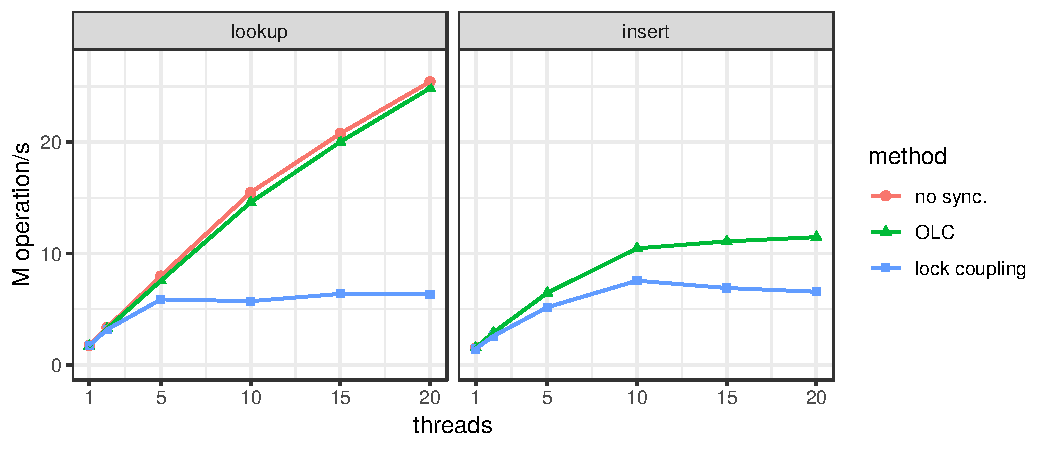
\includegraphics[width=\linewidth]{scale.pdf}
  \vspace{0.2cm}
  \caption{Scalability on 10-core system for B-tree operations (100M values).}
  \label{fig:scale}
\end{figure}

As Figure~\ref{fig:scale} shows, the results change dramatically once we use multiple threads.
For lookup, the scalability of OLC is near-linear up to 20 threads, even though the system has only 10 ``real cores''.
The OLC scalability for insert is also respectable (though not quite as linear because multi-threaded insertion approaches the memory bandwidth of our processor).
The figure also shows that the results of traditional lock coupling with read/write locks are significantly worse than OLC.
With 20 threads, lookup with OLC is 3.9$\times$ faster than traditional lock coupling.

\section{Summary}\label{sec:conc}

Optimistic Lock Coupling (OLC) is an effective synchronization method that combines the simplicity of traditional lock coupling with the superior scalability of lock-free approaches.
OLC is widely applicable and has already been successfully used to synchronize several data structures, including B-trees, binary search trees, and different trie variants.
These features make it highly attractive for modern database systems as well as performance-critical systems software in general.

\begin{thebibliography}{10}

\bibitem{DBLP:conf/spaa/BalmauGHZ16}
O.~Balmau, R.~Guerraoui, M.~Herlihy, and I.~Zablotchi.
\newblock Fast and robust memory reclamation for concurrent data structures.
\newblock In {\em SPAA}, 2016.

\bibitem{DBLP:journals/acta/BayerS77}
R.~Bayer and M.~Schkolnick.
\newblock Concurrency of operations on {B}-trees.
\newblock {\em Acta Informatica}, 9, 1977.

\bibitem{hot}
R.~Binna, E.~Zangerle, M.~Pichl, G.~Specht, and V.~Leis.
\newblock {HOT}: A height optimized trie index for main-memory database
  systems.
\newblock In {\em SIGMOD}, 2018.

\bibitem{DBLP:conf/ppopp/BronsonCCO10}
N.~G. Bronson, J.~Casper, H.~Chafi, and K.~Olukotun.
\newblock A practical concurrent binary search tree.
\newblock In {\em PPOPP}, 2010.

\bibitem{DBLP:conf/vldb/ChaHKK01}
S.~K. Cha, S.~Hwang, K.~Kim, and K.~Kwon.
\newblock Cache-conscious concurrency control of main-memory indexes on
  shared-memory multiprocessor systems.
\newblock In {\em VLDB}, 2001.

\bibitem{intel}
I.~Cutress.
\newblock {Intel} goes for 48-cores: {Cascade-AP} with multi-chip package
  coming soon.
\newblock
  \url{https://www.anandtech.com/show/13535/intel-goes-for-48cores-cascade-ap},
  2018 (accessed January, 2019).

\bibitem{DBLP:conf/cidr/FaleiroA17}
J.~M. Faleiro and D.~J. Abadi.
\newblock Latch-free synchronization in database systems: Silver bullet or
  fool's gold?
\newblock In {\em CIDR}, 2017.

\bibitem{DBLP:journals/ftdb/Graefe11}
G.~Graefe.
\newblock Modern {B}-tree techniques.
\newblock {\em Foundations and Trends in Databases}, 3(4), 2011.

\bibitem{DBLP:conf/hpca/KarnagelDRLLSL14}
T.~Karnagel, R.~Dementiev, R.~Rajwar, K.~Lai, T.~Legler, B.~Schlegel, and
  W.~Lehner.
\newblock Improving in-memory database index performance with
  {Intel}\({}^{\mbox{{\textregistered}}}\) transactional synchronization
  extensions.
\newblock In {\em HPCA}, 2014.

\bibitem{DBLP:journals/tods/LehmanY81}
P.~L. Lehman and S.~B. Yao.
\newblock Efficient locking for concurrent operations on {B}-trees.
\newblock {\em {ACM} Trans. Database Syst.}, 6(4), 1981.

\bibitem{leanstore}
V.~Leis, M.~Haubenschild, A.~Kemper, and T.~Neumann.
\newblock Leanstore: In-memory data management beyond main memory.
\newblock In {\em ICDE}, 2018.

\bibitem{art}
V.~Leis, A.~Kemper, and T.~Neumann.
\newblock The adaptive radix tree: {ARTful} indexing for main-memory databases.
\newblock In {\em ICDE}, 2013.

\bibitem{htmtkde}
V.~Leis, A.~Kemper, and T.~Neumann.
\newblock Scaling {HTM}-supported database transactions to many cores.
\newblock {\em {IEEE} Trans. Knowl. Data Eng.}, 28(2), 2016.

\bibitem{artsync}
V.~Leis, F.~Scheibner, A.~Kemper, and T.~Neumann.
\newblock The {ART} of practical synchronization.
\newblock In {\em DaMoN}, 2016.

\bibitem{DBLP:conf/icde/LevandoskiLS13a}
J.~J. Levandoski, D.~B. Lomet, and S.~Sengupta.
\newblock The {Bw}-tree: A {B}-tree for new hardware platforms.
\newblock In {\em ICDE}, 2013.

\bibitem{DBLP:journals/pvldb/MakreshanskiLS15}
D.~Makreshanski, J.~J. Levandoski, and R.~Stutsman.
\newblock To lock, swap, or elide: On the interplay of hardware transactional
  memory and lock-free indexing.
\newblock {\em {PVLDB}}, 8(11), 2015.

\bibitem{DBLP:dblp_conf/eurosys/MaoKM12}
Y.~Mao, E.~Kohler, and R.~T. Morris.
\newblock Cache craftiness for fast multicore key-value storage.
\newblock In {\em EuroSys}, 2012.

\bibitem{DBLP:journals/tpds/Michael04}
M.~M. Michael.
\newblock Hazard pointers: Safe memory reclamation for lock-free objects.
\newblock {\em {IEEE} Trans. Parallel Distrib. Syst.}, 15(6), 2004.

\bibitem{DBLP:journals/jacm/ShalevS06}
O.~Shalev and N.~Shavit.
\newblock Split-ordered lists: Lock-free extensible hash tables.
\newblock {\em J. {ACM}}, 53(3), 2006.

\bibitem{amd}
A.~Shilov.
\newblock {AMD} previews {EPYC} ‘{Rome}’ processor: Up to 64 {Zen} 2 cores.
\newblock
  \url{https://www.anandtech.com/show/13561/amd-previews-epyc-rome-processor-up-to-64-zen-2-cores},
  2018 (accessed January, 2019).

\bibitem{DBLP:conf/sosp/TuZKLM13}
S.~Tu, W.~Zheng, E.~Kohler, B.~Liskov, and S.~Madden.
\newblock Speedy transactions in multicore in-memory databases.
\newblock In {\em SOSP}, 2013.

\bibitem{buzzword}
Z.~Wang, A.~Pavlo, H.~Lim, V.~Leis, H.~Zhang, M.~Kaminsky, and D.~Andersen.
\newblock Building a {Bw}-tree takes more than just buzz words.
\newblock In {\em SIGMOD}, 2018.

\end{thebibliography}


%\bibliographystyle{abbrv}
%\bibliography{main}

\end{document}

\end{article}
\end{articlesection}

% put the news items below- there can be multiple news sections
% each with its own title
% news will usually have an author as well as a title, 
% e.g. TCDE elections
% news articles are in the same format as letters
% typically, news articles will be stored in a directory called "news"

%\begin{newssection}{News headline}

% insert news items here; news will typically have authors
% see the Sept. 2018 issue for an example

%\begin{news}{news item title}
%{author name}{author affiliation}
%\input{news/news-article.tex}
%\end{news}
%
%\newpage


%\end{newssection}



\begin{callsection}

%  This section will be empty for your version
%
%  Calls for papers section.  Use the callsection environment.
%  Each call for papers is contained in an call environment, where the single 
%  required options to \begin{call} is the name of the conference.
% typically calls are stored in a "calls" directory
%
%\begin{call}{name of conference}
%\centerline{\includegraphics[width=\textwidth, bb= 0 0 590 760]{calls/conference-name.pdf}}
%\end{call}
\begin{call}{ICDE 2019 Conference}
\centerline{
\includegraphics[width=\textwidth, bb= 0 0 610 790] {../Dec-2018/calls/icde19.pdf}} 
%\centerline{
\includegraphics[width=\textwidth, bb= 0 0 590 760] {calls/icde19.pdf}}
\end{call}
\begin{call}{TCDE Membership Form}
%\centerline{\includegraphics[width=\textwidth, bb= 0 0 610 790]
\centerline{
\includegraphics[width=\textwidth, bb= 0 0 590 760] {../Dec-2018/calls/tcde.pdf}}
\end{call}

\end{callsection}

\end{bulletin}
\end{document}
